\documentclass{article}
\usepackage[utf8]{inputenc}
\usepackage{graphicx}
\usepackage{color}
\usepackage{eso-pic}
\usepackage[pages=some]{background}
\usepackage[french]{babel}
\usepackage{lipsum}
\usepackage{array}
\usepackage{geometry}
\usepackage{xcolor}
\usepackage{fancybox}
% \usepackage{natbib}
\usepackage{wrapfig}
\geometry{a4paper,left=25mm,right=25mm,top=25mm}
\usepackage{multicol}
\setlength{\columnsep}{1cm}
\setlength{\parindent}{0pt}
\usepackage[
backend=biber,
style=authoryear,
]{biblatex}
% \usepackage[notes,backend=biber,style=authordate]{biblatex-chicago}
\usepackage{dblfloatfix}
\usepackage{hyperref}
\usepackage{caption}
\usepackage{subcaption}
\usepackage{amssymb}
\usepackage{tocbasic}

\addbibresource{Bibliographie/sources CREDEN.bib}
\AtEveryBibitem{\clearfield{urldate}}
\AtEveryBibitem{\clearfield{langid}}
\AtEveryBibitem{
    \clearfield{urlyear}
    \clearfield{urlmonth}
}
% \AtEveryBibitem{\clearfield{url}}

\title{\centering\huge Projet CREDEN \\~\\ \Large La décarbonation du mix énergétique va-t-elle supprimer les risques géopolitiques ?}
\author{
  CODET, Marie\\
%   \texttt{first1.last1@xxxxx.com}
  \and
  BEAUCOUR, Robinson\\
%   \texttt{first2.last2@xxxxx.com}
}
\date{\today}

\begin{document}
% \AddToShipoutPictureBG*{\includegraphics[width=\paperwidth,height=\paperheight]{BG_electricity.jpg}}

\maketitle
\begin{center}
    
\includegraphics[width=0.8\textwidth]{Images/Intro/PNG-OSE-LOGO-FINAL-1.png}
\end{center}

\begin{abstract}
    La décarbonation du mix énergétique mondial implique des changements majeurs dans les flux physiques mondiaux. Dans un scénario de décarbonation, les flux en combustibles fossiles vont se tarir pour laisser place à une multitude de flux en minéraux. Cette étude propose d'évaluer si les risques géopolitiques d'un mix décarboné seront maîtrisables. Après avoir évalué les risques géopolitiques des ressources en énergies renouvelables, cette étude discute des risques d'approvisionnement de cinq métaux critiques essentiels à la décarbonation : le cuivre, le nickel, le lithium, le cobalt, les terres rares. La suite de la chaîne de valeur est évaluée pour plusieurs technologies bas-carbone : éolien, photovoltaïque, véhicule électrique et réseaux électriques. Une veille sur les politiques publiques sur les métaux critiques est réalisée pour mettre en relief les risques précédents avec les actions qui peuvent avoir été prises par les Etats. Finalement, cette étude discute séparément des risques et des opportunités du nucléaire et de l'hydrogène bas-carbone sur le plan géopolitique.
\end{abstract}

\newpage
\tableofcontents
\clearpage
\listoffigures
\listoftables
% \setcounter{section}{-1}

\newpage
\begin{refsection}
\section*{Introduction}
\addcontentsline{toc}{section}{Introduction}
\begin{figure}[!b]
\centering
    \includegraphics[width=12cm]{Images/Intro/Flux_matières_2050.PNG}
\caption{\centering Quantité totale de matériaux requis pour le système 
énergétique mondial dans un scénario de limitation de réchauffement
climatique à 2°C de l'AIE(\cite{watari_sustainable_2021})}
\label{fig:flux_materiaux}
\end{figure}
En 2015, 197 parties ont signé l'Accord de Paris, qui fixait des objectifs de réduction des émissions de gaz à effet de serre afin de limiter le réchauffement planétaire à moins de 2°C, voire 1,5°C. Fin 2022, 93 pays avaient annoncé un objectif de "zéro émission nette" (\cite{noauthor_net-zero_nodate}). Pour y parvenir, le mix énergétique doit donc être progressivement décarboné. En effet, le secteur de l'énergie - transports compris - était responsable de 75,6\% du total des émissions de gaz à effet de serre en 2019 (\cite{climatewatch_greenhouse}). Le mix énergétique est un bilan par année de la répartition des différentes sources d'énergie primaire, c'est-à-dire les produits énergétiques non transformés, issus de la production et des importations \cite{insee_definition_nodate}. Il peut concerner différentes échelles géographiques : mondiale, nationale, régionale... Au niveau mondial, il était, en 2019, constitué de 31,3\% de pétrole, 26,5\% de charbon, tourbe et pétrole de schiste, et 23,1\% de gaz naturel, soit 80,9\% d'énergies fossiles (\cite{noauthor_greenhouse_nodate}). 
\smallbreak
Cette répartition pose problème car ces énergies représentaient respectivement 33,9\%, 43,4\% et 21,1\% des émissions de gaz à effet de serre provoquées par la combustion de carburant en 2019 (\cite{noauthor_greenhouse_nodate}). Décarboner le mix énergétique signifie donc graduellement diminuer la part des énergies fossiles au profit d'énergies bas carbone. Cela  nécessitera, par ailleurs, une forte amélioration de l'efficacité énergétique, voire l'adoption de la sobriété énergétique. De telles évolutions devraient permettre la réduction de la part des importations d'énergie primaire dans le mix énergétique, notamment grâce à une production plus locale par des sources d'énergies renouvelables, et à l'électrification du secteur des transports. Dès lors, la question suivante se pose : la décarbonation du système énergétique implique-t-elle la fin du risque géopolitique que sous-tendaient les importations d'énergies fossiles?
Selon la discipline sur laquelle on se fonde, la définition du risque varie. De manière générale, il est qualifié comme la possibilité qu'un événement indésirable survienne. La géographie le définit comme la probabilité qu'un aléa se produise et touche une population vulnérable à celui-ci. Cette même discipline fait la différence entre le risque d'origine naturelle, et celui d'origine anthropique, dont fait partie le risque géopolitique (\cite{noauthor_risque_nodate}). Ce dernier s'est aussi développé comme un critère d'évaluation du risque pays, soit l'ensemble des risques auxquels une entreprise est exposée quand elle se projette à l’international, et qui sont susceptibles d'affecter sa profitabilité. 
\smallbreak
Dans ce cadre, le risque géopolitique ne possède pas de définition bien identifiée, mais on pourrait le décrire comme l'ensemble des risques inhérents aux tensions géopolitiques dans un espace donné. Ceux qui nous intéressent particulièrement sont les risques qui pèsent sur les chaînes  d'approvisionnement. Le secteur de l'énergie est stratégique pour tous les Etats, car celle-ci est le fondement du développement économique et de la puissance d’un pays. Ainsi, dans notre étude, nous amalgamerons le risque géopolitique couru par les entreprises à l'international, et celui évalué par les Etats, au regard des potentiels conflits et de la sécurité énergétique. Cette notion désigne l'association de la sécurité nationale et de l'accès aux ressources énergétiques. Elle est l'un des trois enjeux du trilemme énergétique, rejointe par l'équité des prix et la durabilité environnementale. La transition vers une production plus localisée et décarbonée est censée consolider ces piliers.
\smallbreak
Mais plusieurs problématiques viennent infirmer l'hypothèse d'un monde dépourvu de risques géopolitiques grâce à la décarbonation du mix. Soulignons d'abord que les transitions énergétiques ne sont jamais que des empilements de nouvelles sources primaires et des sources prééxistantes. La substitution des secondes par les premières n'est en fait que partielle. Si le pétrole est passé de 46,89\% à 34,2\% du mix entre 1970 et 2017, en valeur absolue, il a connu une augmentation d'environ 102\% sur la même période. Plus qu'à une transition énergétique, nous assistons à un phénomène d'addition énergétique (\cite{hache_vers_2019}). Les risques géopolitiques liés aux approvisionnements en hydrocarbures ne disparaissent donc pas à court terme. Cela est notamment dû au fait que la consommation d'énergie fossile est induite par des usages captifs qui seront explicités dans cette étude. 
\smallbreak
De même, précisons que des systèmes énergétiques qui auraient été entièrement décarbonés reposeraient eux aussi sur des flux de matière, desquels découlent les risques géopolitiques. La figure \ref{fig:flux_materiaux} extraite de (\cite{watari_sustainable_2021}) illustre les changements massifs dans les flux alimentant le système énergétique mondial. 
Cette illustration donne les tendances de la quantité totale de matériaux requis, ce qui peut être défini comme la masse de matière extraite du sol. Cela comprend les matériaux avec un usage économique ainsi que les déchets et les résidus. Par exemple, s'il est nécessaire d'extraire une tonne de roche pour obtenir un kilogramme de cuivre raffiné pour produire une éolienne, la quantité totale de matériaux requis est d'une tonne.\smallbreak
\begin{figure}[!b]
    \centering
    \includegraphics[width=12cm]{Images/Intro/Diversification_métaux.PNG}
    \caption{Diversification des éléments dans l'industrie (\cite{hartard_strategic_2015})}
    \label{fig:divers_metal}
\end{figure}
La figure \ref{fig:flux_materiaux} montre que dans un scénario de décarbonation intense, la transition énergétique conduit, d'une part, à un changement des flux de matériaux requis avec une part des combustibles fossiles qui baisse en faveur de la part des métaux. D'autre part, le flux de matériaux décroît en valeur absolue, bien que (\cite{watari_sustainable_2021}) ne prennent pas en compte le développement des réseaux électriques. Ce point sera développé dans cette étude. Cet indicateur de flux, bien qu'insuffisant pour décrire l'évolution des risques géopolitiques, permet de préfigurer des mutations à venir. Une autre tendance à prendre en compte est la complexification de nos systèmes énergétiques, dans lesquels la technologie et sa maîtrise jouent un rôle plus important. Cette complexification s'illustre en figure \ref{fig:divers_metal} avec la  diversification des métaux dans l'industrie, qui est une conséquence de systèmes complexes. Dans ce contexte, même des flux minimes de matériaux, quand ils sont compilés, peuvent impacter le développement des systèmes énergétiques.
Ces changements dans les flux et dans les technologies sont à l'origine de mutations dans le risque géopolitique sur les systèmes électriques que nous discuterons dans cette étude.
\smallbreak
Un monde décarboné implique-t-il une meilleure maîtrise des risques géopolitiques ? Il est difficile d'apporter une réponse quantifiable à cette question, et la littérature n'est pas unanime à ce sujet. L'état de cette dernière a déterminé le périmètre de notre rapport.
\smallbreak
Si la décarbonation du mix énergétique n'implique pas la fin des risques géopolitiques, à quelles mutations peut-on s'attendre ? Quelles seront les solutions d'atténuation des risques géopolitiques mises en place pour sécuriser les approvisionnements énergétiques ?
\smallbreak
Ce rapport traitera d'abord des risques découlant de la recrudescence des sources renouvelables dans les mix énergétiques, pour les pays exportateurs comme importateurs d'électricité. Ensuite, il sera question des approvisionnements en matériaux critiques de la transition énergétique, de la maîtrise technologique et industrielle induite par cette dernière, et des politiques de sécurisation des matériaux susnommés. Enfin, nous étudierons les risques géopolitiques inhérents au développement de l'énergie nucléaire et de l'hydrogène, voués à gagner en importance dans le mix en vue de sa décarbonation.

\vfill
\printbibliography
\clearpage
\end{refsection}

% 1
\begin{refsection}
\section{Des risques géopolitiques pour les renouvelables?}
\addxcontentsline{myelements}{subsection}{My Custom Element}

    Le risque de conflits entourant les gisements et les moyens de production énergétique est une préoccupation majeure de la géopolitique des hydrocarbures. Cependant, il existe un débat dans la littérature concernant la quantité et la nature des risques pesant sur la sécurité des systèmes énergétiques décarboné (\cite{vakulchuk_renewable_2020}). Un groupe d'auteurs avance que la transition vers un mix décarboné sera synonyme d'une réduction des conflits inter-étatiques liés à l'énergie, notamment du fait d'une plus grande indépendance énergétique. À l'opposé, d'autres font l'hypothèse que ces conflits perdureront. On peut distiguer deux courants de pensée dans ce dernier groupe. Il y a d'abord ceux pour qui lesdits risques seront les mêmes que dans un monde dépendant des hydrocarbures, soit les ruptures d'approvisionnement ou encore l'instabilité géopolitique dans les pays producteurs. Enfin, certains auteurs théorisent une mutation de ces risques, en particulier vers un déplacement de ces derniers vers les matériaux critiques, que nous étudierons dans la partie suivante.
\smallbreak
Penchons-nous d'abord sur les hypothèses entourant la possibilité de conflits relatifs à la production d'énergie renouvelable dans un contexte de mix décarboné. Dans cette étude, nous nous sommes concentrés sur trois grandes catégories de risques qui pourraient causer ou faciliter ces derniers : l'utilisation de l'énergie renouvelable comme une arme géopolitique, la malédiction des ressources, et la cyber-vulnérabilité. Nous retirons de cette analyse que l'évaluation des risques traditionnellement afférents à l'approvisionnement en énergie doit évoluer pour prendre en compte les mutations apportées par la transition énergétique.
    \subsection{Les renouvelables comme arme géopolitique}
    \label{section:arme}
    Premièrement, peut-on affirmer que l'énergie renouvelable pourra servir d'arme géopolitique ? Cette question est particulièrement pertinente du fait du stress pesant aujourd'hui sur les économies européennes du fait de la diminution des livraisons de gaz naturel en provenance de la Russie, dont on peut supposer qu'elle est une mesure de représailles face au soutien indirect de l'Union européenne (UE) à l'Ukraine. Il est possible d'émettre l'hypothèse que si les risques inhérents à la consommation d'énergie fossile sont perpétués dans des systèmes décarbonés, l'usage des renouvelables comme un moyen de pression pourrait être envisageable. Selon (\cite{raman_fossilizing_2013}), les technologies de production des énergies renouvelables se "fossilisent", c'est-à-dire que le fonctionnement de leur économie politique devient semblable à celle des fossiles. Elles deviendraient, de ce fait, une nouvelle source de tensions géopolitiques.  
\smallbreak
En outre, dans le cas larges réseaux d'électricité interconnectés, de potentielles tensions les entourant entre voisins conflictuels ne peuvent être écartées, car les interdépendances ne disparaîtront pas. Si ces dernières se manifestaient auparavant entre des zones très éloignées géographiquement, dans le futur, elle concerneront des pays proches, du fait de l'intermittence des énergies comme le solaire ou l'éolien. (\cite{fischhendler_geopolitics_2016}) ont étudié les réseaux électriques transfrontaliers entre Israël et ses voisins. Ils en ont déduit que lorsque les politiques nationales sont motivées par la paix, les propositions d'interconnexion se multiplient. Seulement, quand les relations entre ces Etats se détériorent, les projets sont reconsidérés ou "pris en otage" par des politiques jugées plus vitales. Dans le cas israélo-arabe, la géopolitique de l'électricité a constitué un tremplin pour la coopération internationale, mais aussi une forme de moyen de pression.
\smallbreak
Cependant, ces arguments ne prouvent pas exactement que l'énergie renouvelable puisse être un levier de coercition ou de représailles comme l'exemple de la Russie précédemment cité. En réalité, du fait de la nature décentralisée, de leur meilleure répartition géographique (\cite{overland_are_2022}) et de la probable bi-directionnalité des échanges de renouvelables (\cite{leonard_resource_2022}), elles pourront difficilement être utilisées comme arme géopolitique. Ainsi, (\cite{overland_geopolitics_2019}) considère que cela serait même un "mythe", dans la mesure où les relations commerciales entre Etats seront plus symétriques grâce à l'apparition des pays prosumers, c'est-à-dire qui consommeront leur propre production. Si une asymétrie subsiste, elle serait différente de celle qui existe actuellement, car les pays importateurs auront la solution de développer leur potentiel renouvelable dans une certaine mesure. Cette nouvelle concurrence inciterait les producteurs à être plus arrangeants avec leurs clients. Cela renforcerait donc la sécurité énergétique des pays importateurs, sous réserve que soient adoptées des mesures visant à atténuer les risques régulatoires qui pourraient peser sur les échanges internationaux d'énergie renouvelable (\cite{escribano_frances_res_2013}).
    \subsection{Malédiction des ressources}
    \label{section:malédiction}
    \input{01 - Nouveaux risques ENR/02 - malédiction.tex}
    \subsection{Vulnérabilité au risque cyber}
    \label{section:cyber}
    La décarbonation et la digitalisation des économies ont souvent été présentés comme des processus jumeaux ; la transition énergétique est même dépendante de la transition numérique, en raison des nouveaux besoins de pilotage et d'interconnexion des réseaux (\cite{iea_digitalization_2017}, \cite{commission_europeenne_twin_2022}, \cite{unep_digitalisation_2021}). Pour certains auteurs, cela implique le renforcement des risques cyber autour des infrastructures énergétiques (\cite{eyl-mazzega_dimension_2019}). En décembre 2015, l'Ukraine a été victime d'une cyberattaque visant trois de ses gestionnaires de distribution d'électricité (\cite{zetter_inside_2016}). Celle-ci, qui a résulté en l'arrêt de 30 sous-stations électriques, a provoqué une importante coupure dans l'ouest du pays, confirmant les craintes entourant la digitalisation des réseaux énergétiques. S'il est fréquent que les gestionnaires de réseaux électriques soient la cible d'attaques cyber, il convient toutefois de noter que l'Ukraine reste un cas particulier pour plusieurs raisons. Ses infrastructures étaient vétustes, le pays présente un haut niveau de corruption, et était alors en conflit militaire larvé avec la Russie, sachant que les réseaux ukrainiens et russes sont fortement interconnectées (\cite{overland_geopolitics_2019}).
\smallbreak
De plus, on peut supposer que même si la transition énergétique conduira à plus de digitalisation, l'effet de décentralisation des réseaux conduira à une plus grande résilience face au risque cyber, car cela induit la démultiplication des cibles à hacker afin de faire tomber un système en entier. Sans compter que les recherches et les politiques liées à la cybersécurité, découlant des expériences passées d'attaques et de la peur qu'elles ont engendré, ont permis l'implémentation de contre-mesures (\cite{overland_geopolitics_2019}).
    \subsection{Vers une nouvelle grille d'analyse ?}
    \label{section:analyse}
    Ainsi, la géopolitique des énergies renouvelables ne saurait être comprise en l'analysant uniquement avec la grille traditionnellement appliquée aux hydrocarbures. En examinant les risques majeurs pouvant mener au conflit, ou l'accentuer - soit l'utilisation de l'énergie comme arme géopolitique, la malédiction des ressources et la vulnérabilité cyber -, on peut souligner qu'aucun d'entre eux ne s'applique pleinement à des systèmes énergétiques décarbonés. Nous assistons actuellement à un glissement d'une compétition pour les ressources énergétiques et les zones géographiques vers une rivalité autour de la maîtrise technologique et les droits de propriété intellectuelle (\cite{hache_vers_2019}, \cite{overland_geopolitics_2019}). L'apparition progressive d'acteurs non-étatiques dans la géopolitique des énergies force également le changement de perspective sur l'analyse du risque de conflits (\cite{mansson_resource_2015}). 
\smallbreak
On peut illustrer cette complexification à travers une analogie historique. La géopolitique des énergies était auparavant comparable à la Guerre Froide, dans la mesure où les confrontations étaient nombreuses, mais il existait deux pôles définis du pouvoir : les Etats-Unis et l'Union soviétique. Le jeu des alliances et les négociations étaient donc définies dans ce cadre. Le secteur des hydrocarbures présente également des acteurs identifiés et reconnaissables. La géopolitique des énergies renouvelables est, elle, assimilable au monde post-Guerre Froide, du fait des incertitudes autour des enjeux, et de la multiplicité des centres et des acteurs (\cite{paltsev_complicated_2016}).
\smallbreak
Toutefois, l'évaluation des risques "traditionnelle" est plus cohérente avec l'étude de la géopolitique des matériaux critiques de la transition énergétique. Leur nature non renouvelable, leur concentration géographique, leur caractère stratégique et la notion de stocks sont des caractéristiques qu'ils partagent avec les énergies fossiles. 
    \clearpage
    \printbibliography
    \clearpage
\end{refsection}
% 2
\section{Approvisionnement en métaux}
\label{section:approvisionnement}
    Le risque de conflits entourant les gisements et les moyens de production énergétique est une préoccupation majeure de la géopolitique des hydrocarbures. Cependant, il existe un débat dans la littérature concernant la quantité et la nature des risques pesant sur la sécurité des systèmes énergétiques décarboné (\cite{vakulchuk_renewable_2020}). Un groupe d'auteurs avance que la transition vers un mix décarboné sera synonyme d'une réduction des conflits inter-étatiques liés à l'énergie, notamment du fait d'une plus grande indépendance énergétique. À l'opposé, d'autres font l'hypothèse que ces conflits perdureront. On peut distiguer deux courants de pensée dans ce dernier groupe. Il y a d'abord ceux pour qui lesdits risques seront les mêmes que dans un monde dépendant des hydrocarbures, soit les ruptures d'approvisionnement ou encore l'instabilité géopolitique dans les pays producteurs. Enfin, certains auteurs théorisent une mutation de ces risques, en particulier vers un déplacement de ces derniers vers les matériaux critiques, que nous étudierons dans la partie suivante.
\smallbreak
Penchons-nous d'abord sur les hypothèses entourant la possibilité de conflits relatifs à la production d'énergie renouvelable dans un contexte de mix décarboné. Dans cette étude, nous nous sommes concentrés sur trois grandes catégories de risques qui pourraient causer ou faciliter ces derniers : l'utilisation de l'énergie renouvelable comme une arme géopolitique, la malédiction des ressources, et la cyber-vulnérabilité. Nous retirons de cette analyse que l'évaluation des risques traditionnellement afférents à l'approvisionnement en énergie doit évoluer pour prendre en compte les mutations apportées par la transition énergétique.
    \subsection{Définition de la criticité}
    Un matériau n'est pas critique seulement parce qu'il est rare. (\cite{geldron_lepuisement_2017}) différencie justement plusieurs types de métaux. D'abord, les métaux rares et très rares sont catégorisés par leur concentration dans la croûte terrestre qui est comprise entre 1 et 1000 ppm pour les premiers (cuivre, nickel, cobalt...), et inférieure à 1 ppm pour les seconds (platinoïdes...). Les petits métaux sont classés ainsi du fait des faibles volumes produits et de la taille du marché. Les métaux dits stratégiques sont considérés comme tels par des entreprises, des Etats, ou par des secteurs, selon le degré de leur dépendance. Enfin, les métaux critiques le sont du fait d'un épisode d'embargo, ou de menaces émises par un pays producteur.
\smallbreak
La criticité est communément déterminée selon deux critères. Premièrement, elle l'est à partir de l'évaluation du risque d'approvisionnement, qui se caractérise par des aspects techniques, économiques, régulatoires et politiques. Secondement, la vulnérabilité à la restriction des approvisionnements est examinée, c'est-à-dire les conséquences économiques d'une baisse, la substituabilité du métal, et son importance stratégique (\cite{hatayama_adopting_2018}). Par exemple, en France, c'est cette méthodologie d'évaluation qui est appliquée. Le Comité pour les métaux stratégiques mesure le risque d'approvisionnement à travers une cartographie des flux de la chaîne d'approvisionnement, de l'extraction à la production de métal. Quant à la vulnérabilité au risque susnommé, elle est estimée à partir d'échanges avec les fédérations professionnelles et les acteurs industriels (\cite{comes_note_2018}). 
\smallbreak
Ces deux critères sont aussi les axes des matrices d'évaluation des risques, soit la probabilité d'occurence d'un risque, et la sévérité des conséquences en cas de réalisation. La première de ces matrices a été établie en 2008 aux Etats-Unis (\cite{hache_vers_2019}). Il faut donc mettre en avant le lien entre la mesure de la criticité et la recherche du maintien de la puissance. Cela passe aujourd'hui par la maîtrise des technologies de pointe, très dépendantes de la disponibilité de multiples métaux, expliquant ainsi leur caractère stratégique.
\smallbreak
(\cite{hache_vers_2019}) complètent ces définitions des matériaux critiques. Ces derniers sont utiles à de multiples secteurs de l'industrie, sont peu substituables, leurs usages industriels croissent dans le temps, leur potentiel de recyclage est limité, leur valeur économique est élevée, leur production et leurs réserves sont concentrées géographiquement et les produire peut engendrer des externalités négatives sur l'environnement (voir figure \ref{fig:criticite}).
\begin{figure}
    \centering
    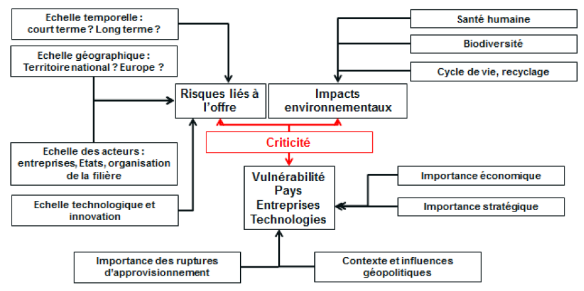
\includegraphics[width=0.8\textwidth]{Images/02 appro/schema criticite.png}
    \caption{Evaluer la criticité des matières premières. Source : \cite{hache_vers_2019}}
    \label{fig:criticite}
\end{figure}
Les auteurs font état d'une multiplicité d'indicateurs utilisés dans la littérature pour mesurer la criticité, qu'ils classent, conformément à la définition citée au paragraphe précédent, entre ceux relatifs à la vulnérabilité économique et ceux rattachés aux risques sur l'offre, sachant que certains peuvent appartenir aux deux groupes. Les premiers peuvent être ordonnés dans les sous groupes suivants : mesure de la dépendance (importance stratégique, dépendance aux importations, volume de la consommation...), valeur économique (valeur des produits affectés, valeur des matériaux utilisés) et substituabilité et recyclage (recyclabilité du produit, existence d'un substitut, capacité à innover...). Quant aux seconds, ils peuvent être groupés ainsi : indicateurs géologiques et physiques (dépendance aux coproduits, présence dans la croûte terrestre, vulnérabilité au changement climatique...), indicateurs économiques et financiers (investissements dans le secteur minier, volatilité des prix des matières premières, existence d'un marché financier...), indicateurs stratégiques (concentration par pays et des entreprises, risque d'embargo...) et enfin substituabilité et recyclage (potentiel de recyclage, existence d'un substitut). En outre, il existe actuellement une discussion dans la communauté scientifique autour de l'ajout d'un troisième axe dans l'évaluation de la cricité : les conséquences environnementales de la production d'un matériau. Cela pose en effet la question de l'indépendance des enjeux qui en découlent par rapport aux ruptures d'approvisionnement et à la vulnérabilité économique.
\smallbreak
Dans l'ensemble, il ressort de la littérature que la criticité est une notion complexe, dont la pluridisciplinarité des approches et la multiplicité des horizons temporels choisis rend difficile la comparaison entre études. Dès les années 1970, le débat sur la déplétion des ressources subvenu entre les auteurs du rapport \textit{The Limits to Growth} issus de la dynamique des systèmes et des économistes, dont Friedrich Hayek, en est la preuve. (\cite{tilton_assessing_2003}) s'est appuyé sur cette controverse pour formuler l'existence de deux paradigmes. D'abord, il énonce celui des géologues raisonnant à partir de stocks non-renouvelables de ressources et considérant les limites de ceux-ci face à une demande grandissante dans le temps. Il le compare au paradigme des économistes, qui fondent leur réflexion sur la notion de coût d'opportunité. Dans cette approche, l'accent est plus mis sur les substituts, le recyclage, et l'élasticité-prix de la demande. Si les géologues prennent en compte le très long terme, les économistes réfléchissent avec le temps des cycles économiques, c'est-à-dire les court et moyen termes. Pour Tilton, la déplétion économique due à un effondrement de la demande face à une hausse des prix des matières premières est plus envisageable qu'une déplétion géologique. (\cite{hache_vers_2019}) notent toutefois que cet auteur n'a pas théorisé ces paradigmes dans le cadre de la transition énergétique.


    \label{section:criticité}
\clearpage
\subsection{Fiches métaux}
\label{section:fiches}
L'approvisionnement d'une multitude de métaux peut être étudié. Cinq métaux particulièrement critiques pour les technologies bas-carbone sont revus dans cette étude. Le contexte de chaque métal est donné dans les fiches suivantes.
Chaque fiche est introduite par un diagramme en barre horizontal. Ce diagramme utilise les dernières données disponibles pour exposer la répartition des réserves, de la production minière (extraction), de la production de métal raffiné (production) et éventuellement de la consommation.\\
\\
Sources des fiches métaux : \cite{brgm_fiche_2016},\cite{brgm_fiche_2016-1},\cite{brgm_fiche_2017},\cite{brgm_fiche_2018},\cite{brgm_fiche_2021},\cite{iea_role_2021}, \cite{usgs_rare_2021}

\begin{center}
    \boxput*(0,1){
        \colorbox{white}{Scénarios AIE}
    }{
    \setlength{\fboxsep}{15pt}
    \fbox{\begin{minipage}{14cm} 
    Plusieurs scénarios sont envisagés dans les publication de l'agence internationale de l'énergie.\\
    \\
    \textbf{STEPS} pour "Stated Policies Scenario". Le STEPS fournit une référence plus prudente pour l'avenir, car il ne tient pas pour acquis que les gouvernements atteindront tous les objectifs annoncés.\\
    \textbf{APS} pour "Announced Pledges Scenario". Un scénario qui suppose que tous les engagements climatiques pris par les gouvernements du monde entier, y compris les contributions déterminées au niveau national et les objectifs de zéro net à plus long terme, ainsi que les objectifs d'accès à l'électricité.\\
    \textbf{SDS} pour "Sustainable Development Scenario". SDS est un scénario normatif utilisé pour modéliser une trajectoire "bien en dessous de 2°C" ainsi que la réalisation d'autres objectifs de développement durable.\\
    \textbf{NZE} pour "Net Zero Emission by 2050". Un scénario qui définit une voie pour que le secteur mondial de l'énergie atteigne zéro émission nette de CO$_2$ d'ici 2050. Il ne s'appuie pas sur les réductions d'émissions extérieures au secteur de l'énergie pour atteindre ses objectifs. Il implique l'accès universel à l'électricité d'ici 2030.\\
    \\
    Source : \cite{iea_global_2022}
    
    \end{minipage}}
    }
\end{center}

\begin{figure}[!b]
    \centering
    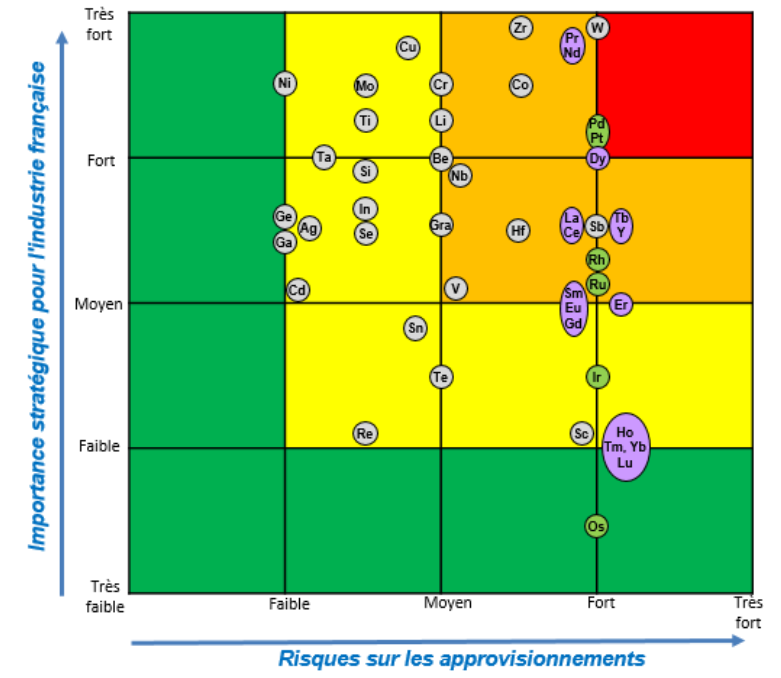
\includegraphics[width=0.6\textwidth]{Illustration métaux/martice.png}
    \caption{Criticite des métaux en France d'après \cite{brgm_marche_nodate}}
    \label{fig:my_label}
\end{figure}
\clearpage
\begin{center}
\subsubsection*{Cuivre}
\addcontentsline{toc}{subsubsection}{Cuivre}
\end{center}

\begin{center}
    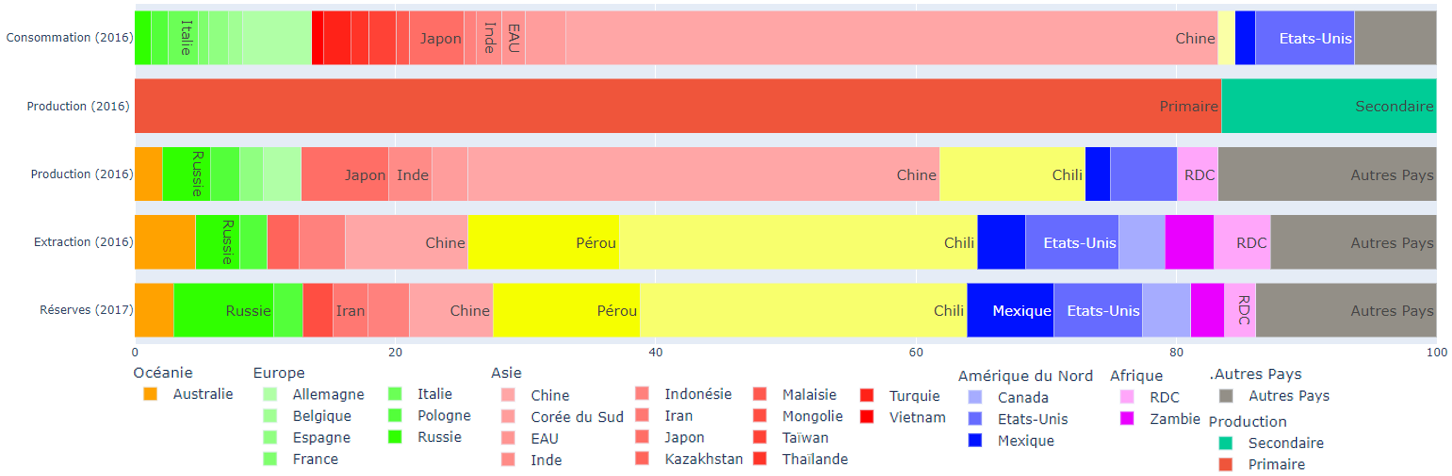
\includegraphics[width=\textwidth]{Illustration métaux/Cuivre.png}
\end{center}
\begin{center}
    \textbf{Usages et consommation}
\end{center}
La demande en cuivre est relativement corrélée au développement économique matériel global (construction, infrastrucure, équipements).
La consommation de cuivre raffiné de la Chine dépasse sa production bien qu'étant le premier pays producteur.
\begin{center}
    \textbf{Prospective}
\end{center}
\begin{multicols}{2}
    \begin{center}
        \textit{Total copper demand by sector and scenario}
    \end{center}
    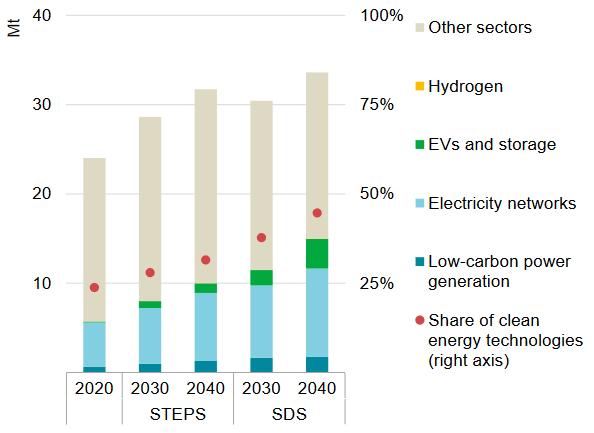
\includegraphics[width=0.45\textwidth]{Illustration métaux/Cuivre prospective.PNG}
    \vfill\null
    \columnbreak
    Il est prévu que la demande de cuivre augmente à cause du développement 
    économique mondial et de la décarbonation. Selon certains scénarios, la part de la consommation de
     cuivre pour les technologies bas-carbone
    pourrait passer de 25\% à 40\% en 2040. La demande en cuivre pour la décarbonation est
    soutenue par le développement des réseaux électriques (en particuliers distributions), 
    des véhicules électriques, des moyens de production bas-carbone.
    Les projets actuels d'extraction permettent de satisfaire la demande dans les prochaines années mais de nouveaux projets
    sont nécessaires pour satisfaire la demande à partir de 2028. La décroissance de la concentration en minerai de cuivre dans les mines
    pourrait augmenter le coût et l'impact environnemental de l'extraction.
\end{multicols}
\begin{center}
    \textbf{Production et Recyclage}
\end{center}
La production minière de cuivre a connu un taux de croissance annuel moyen de 3.25\% entre 1900 et 2016. La production minière dépasse 20 Mt/an. Cependant, les mines actuelles
sont proches de leur pic de production. La production secondaire de cuivre est passée de 2 Mt/an en 2000 à 4Mt/an en 2015.
La production secondaire a été de 42kt en 2014 pour la France sur une consommation de 248kt. La France exporte de l'ordre de 200 kt de
déchets cuivreux et en importe 50kt.
\begin{center}
    \textbf{Substituabilité}
\end{center}
Les performances électriques et thermiques du cuivre le rendent difficile à substituer. Les moteurs électriques à aimant permanent
(utilisant des terres rares) consomment moins de cuivre. Il est possible d'avoir des câbles électriques (en particulier pour les lignes aériennes)
en aluminium (moins conducteur mais plus léger).
\begin{center}
    \textbf{Prix}
\end{center}
Le prix du cuivre est assez stable. En moyenne à 6 166 US\$/t en 2017 il a atteint un pic à 10 500 US\$/t début 2022
au London Metal Exchange. La valeur de marché de la production métallurgique annuelle de cuivre est de l'ordre de 150 G US\$.

\clearpage
\begin{center}
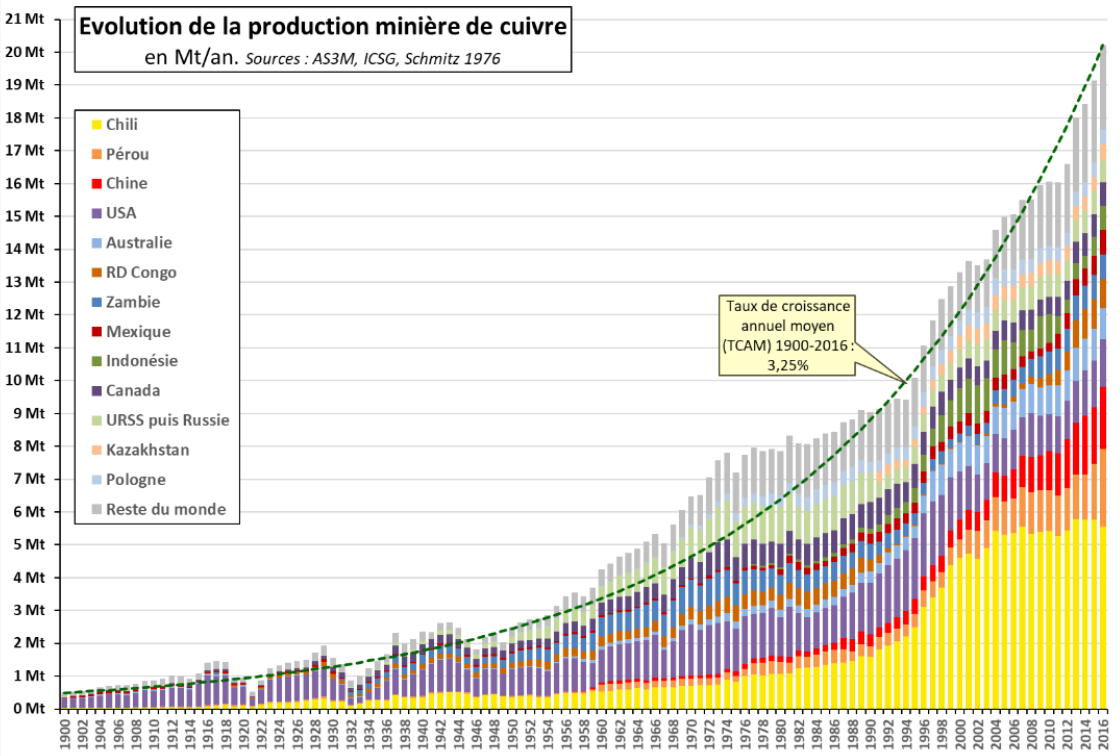
\includegraphics[width=0.7\textwidth]{Illustration métaux/Dynamique_cuivre.png}
\end{center}
\begin{center}
    \textbf{Evènements géopolitiques}
\end{center}
Il n'y a pas eu d'évènements géopolitiques notables entre 2000 et 2020.

\begin{multicols}{2}
    \begin{center}
      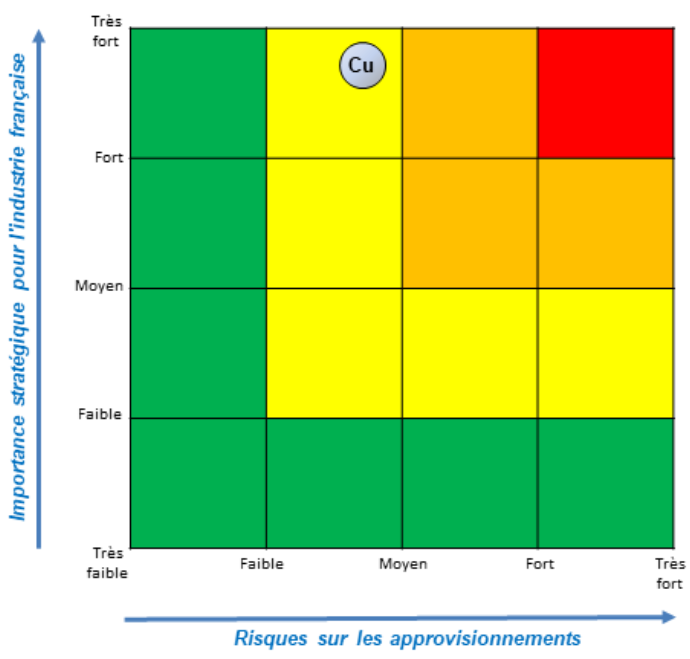
\includegraphics[width=0.35\textwidth]{Illustration métaux/Cuivre_criticité.png} 
    \end{center}
    \begin{center}
    \textbf{Criticité en France}
    \end{center}
    Le risques sur les approvisionnements en cuivre est assez faible du fait de la diversification des producteurs
    métallurgiques et miniers ainsi que de l'abondance du métal. Cependant ce métal est très fortement important pour
    la décarbonation du mix énergétique et pour l'industrie en général.
\end{multicols}

\begin{center}
\textbf{Risques spécifiques}
\end{center}
Le cuivre et le lithium sont des métaux particulièrement exposés aux stress hydriques avec la moitié de la production située dans des zones à fort stress hydrique. L'accentuation du stress hydrique par le changement climatique commence déjà à perturber l'approvisionnement par le Chili ou l'Australie.
\begin{center}
    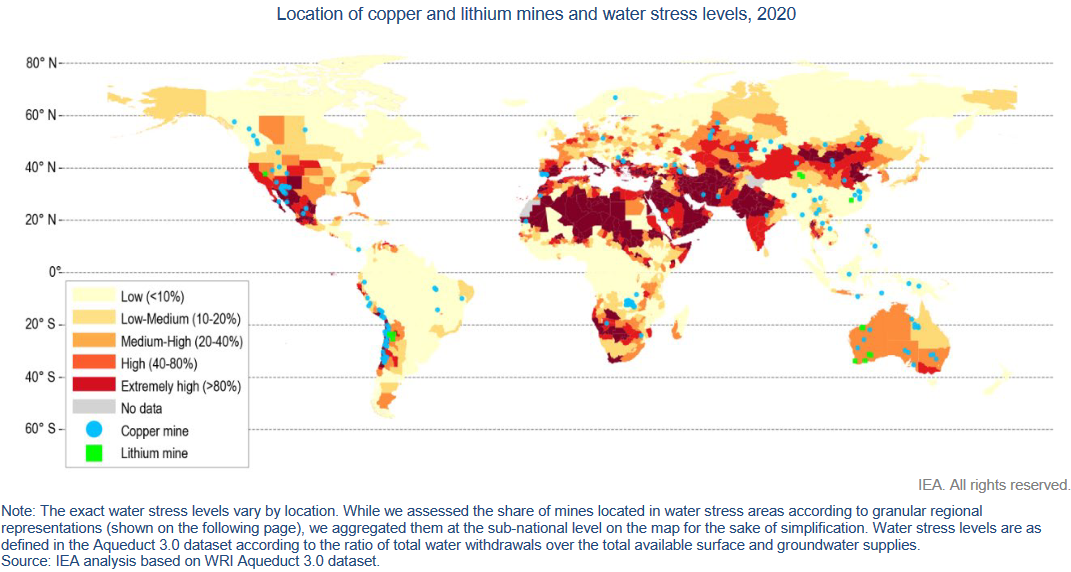
\includegraphics[width=0.75\textwidth]{Illustration métaux/risque_hydrique_cuivre.png} 
\end{center}

\begin{center}
\subsubsection*{Nickel}
\addcontentsline{toc}{subsubsection}{Nickel}
\end{center}
\begin{center}
    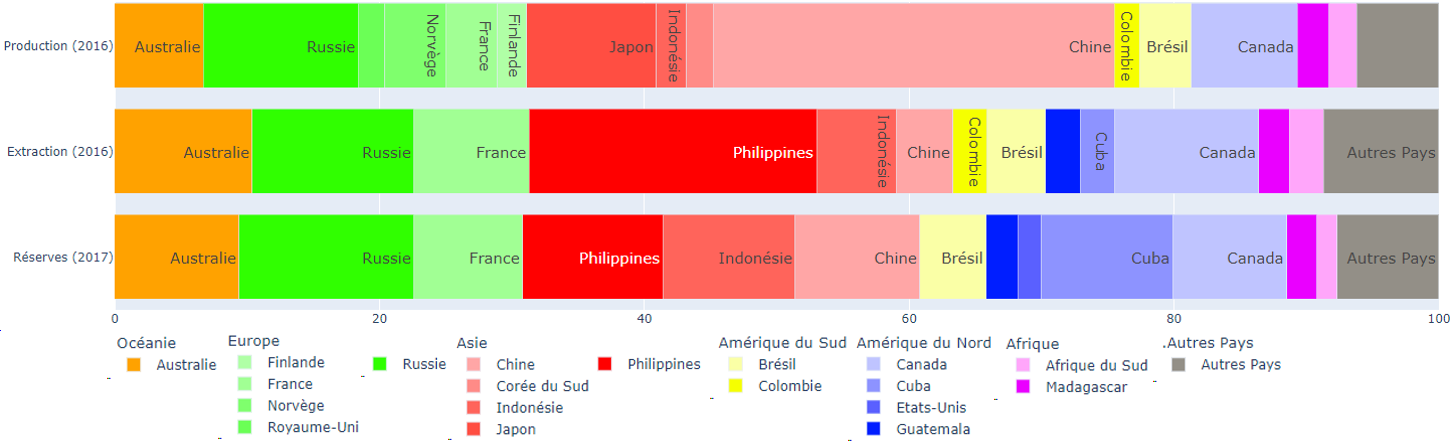
\includegraphics[width=\textwidth]{Illustration métaux/Nickel.png}
\end{center}
\begin{center}
    \textbf{Usages et consommation}
\end{center}
Le nickel est utilisé à 85 \% pour la production d'acier inoxydable ou d'autres alliages. Moins de 7 \% du nickel est actuellement
utilisé pour la production de batterie. Dans le domaine énergétique, le nickel est très critique pour
la géothermie, le stockage d'hydrogène et la fabrication de batteries. Il est modérément critique pour l'énergie
nucléaire, éolienne et solaire à concentration.

\begin{center}
    \textbf{Prospective}
\end{center}
\begin{multicols}{2}
    \begin{center}
        \textit{Total nickel demand by sector and scenario}
    \end{center}
    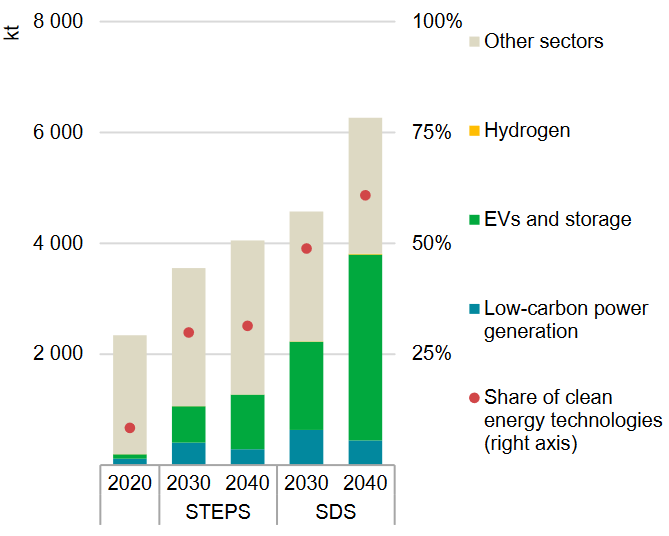
\includegraphics[width=0.45\textwidth]{Illustration métaux/Nickel prospective.PNG}
    \vfill\null
    \columnbreak
    La demande en inox est corrélée au développement économique global. Cependant dans les prochaines années
    la demande en nickel pourrait être fortement stimulée par la fabrication de batterie. Les technologies
    bas-carbone représentent actuellement une faible part de la demande de nickel, mais cette part est amenée à fortement augmenter dans les deux prochaines décennies dépassant 50\% de la demande. Le marché est amené à être bien approvisionné dans les prochaines années, même si des tensions sont possibles avec l'augmentation rapide de la demande en nickel de classe 1 (pur à plus de 99.8\%).
\end{multicols}
\begin{center}
    \textbf{Production et recyclage}
\end{center}
La production minière de nickel a augmenté chaque année en moyenne de 3.93\% de 1945 à 2015. La production minière est de l'ordre de 2 200 kt/an. Le nickel est peu recyclé
en tant que tel, mais les inox et alliages contenant du nickel sont fortement recyclés. Sous toutes ses formes
le taux de recyclage en fin de vie du nickel est d'environ 60\% à l'échelle mondiale. La production minière de La
Nouvelle-Calédonie dont la production est raffinée sur place ou dans la métropole représente 8.7\% de la production mondiale.
\begin{center}
    \textbf{Substituabilité}
\end{center}
Le nickel dans les alliages est difficilement substituable sans contrepartie économique ou technique. L'abondance
et les prix actuels du nickel n'incitent pas à d'avantage de recherches pour la substitution. Des technologies
de batteries avec moins ou pas de nickel sont actuellement matures. 
\begin{center}
    \textbf{Prix}
\end{center}
La volatilité du prix du nickel est modérée. En moyenne à 9 500 US\$/t en 2016, le prix du nickel a atteint un pic très temporaire
à 43 000 US\$/t début 2022 avant la fermeture temporaire du marché pendant l'invasion russe en Ukraine. La valeur du marché de la production métalurgique annuelle de nickel est de l'ordre de 19 G US\$.

\clearpage
\begin{center}
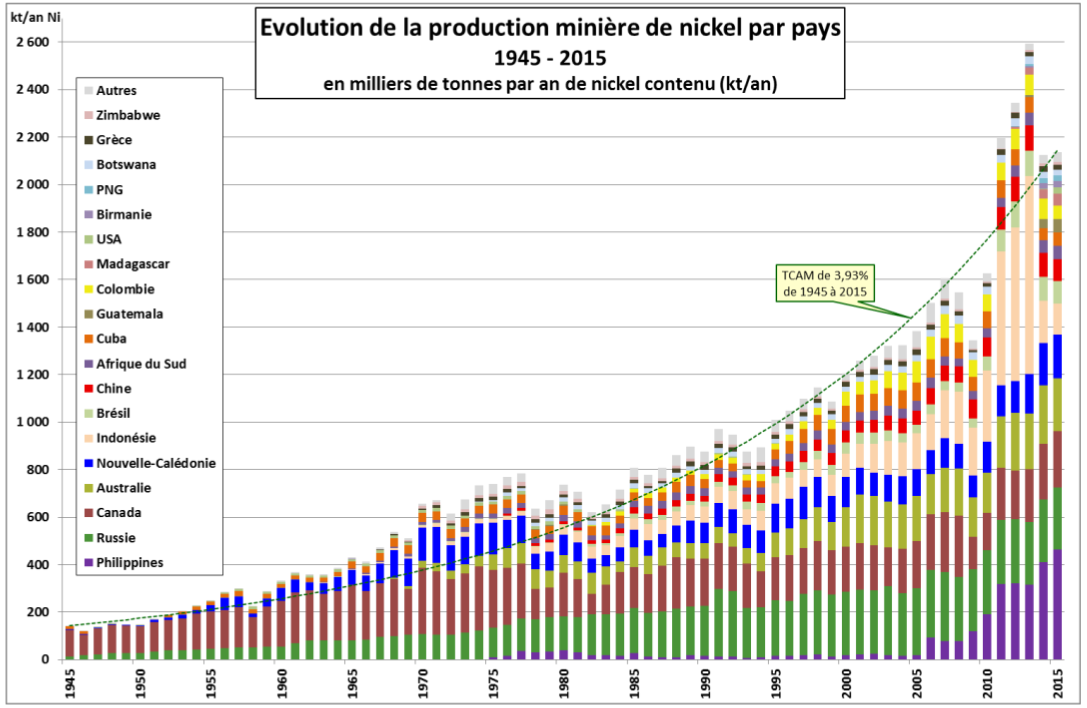
\includegraphics[width=11cm]{Illustration métaux/Dynamique_nickel.png}
\end{center}
\begin{center}
    \textbf{Evènements géopolitiques}
\end{center}
L'Indonésie était le premier producteur minier mondial en 2013 avec 32\% de la production. Le pays est passé au sixième rang en 2015 à la suite de l'embargo décidé sur les exportations de minerai brut entre janvier 2014 et 2017. L'Indonésie a décidé de nouvelles restrictions à partir de 2020 (voir encadré \hyperref[Indonesia]{\textit{L’Indonésie et le nickel : existe-t-il un risque de cartellisation ?}}). 

\begin{multicols}{2}
    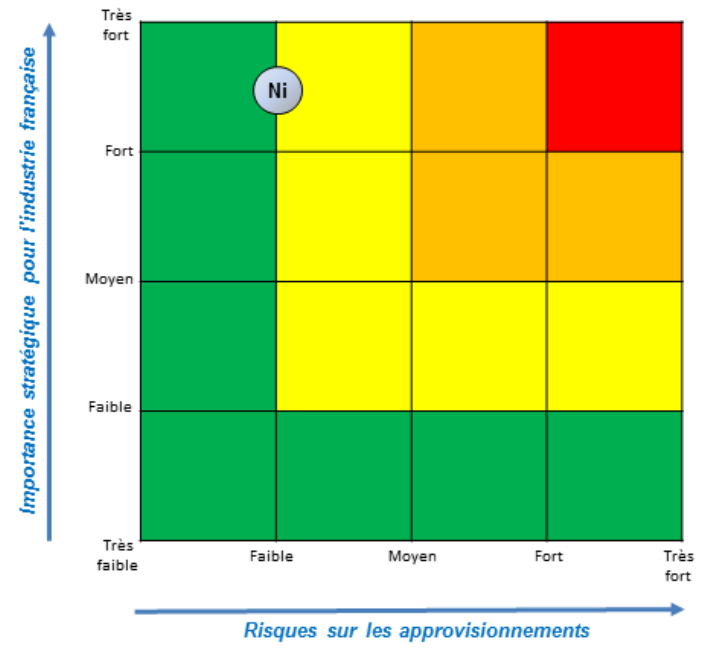
\includegraphics[width=0.35\textwidth]{Illustration métaux/Nickel_criticité.png}
    \begin{center}
    \textbf{Criticité en France}
    \end{center}
    Le risque sur les approvisionnements en nickel est faible en France grâce à la faible concentration
    du marché mondial et grâce à la production en Nouvelle-Calédonie. Il n'empêche que ce métal est peu substituable
    et particulièrement important dans l'économie.
\end{multicols}

\begin{multicols}{2}
    \begin{center}
        \textit{Chaîne d'approvisionnement du nickel}
    \end{center}
    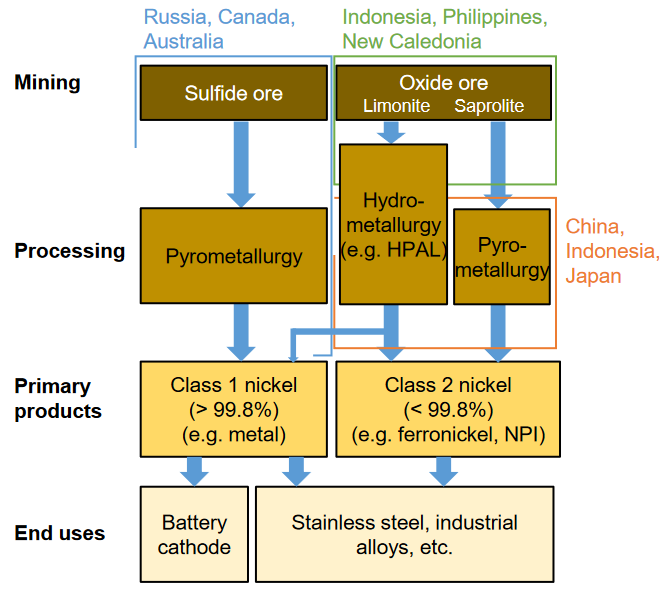
\includegraphics[width=0.45\textwidth]{Illustration métaux/Nickel_supply_chain.PNG}
    \begin{center}
    \textbf{Risques spécifiques}
    \end{center}
    Le nickel raffiné se sépare en deux classes : classe 1 pour une pureté supérieure à 99.8\%, classe 2 sinon.
    Le nickel de classe 1 uniquement peut être utilisé dans les batteries. Seule la production d'un certains type 
    de réserves ("sulfide ore") permet facilement d'acquérir du nickel de classe 1. Le raffinage en classe 1 de
    nickel issu d'autres réserves ("Oxide ore") est actuellement très difficile technologiquement et très onéreux.
\end{multicols}


\begin{center}
\subsubsection*{Lithium}
\addcontentsline{toc}{subsubsection}{Lithium}
\end{center}
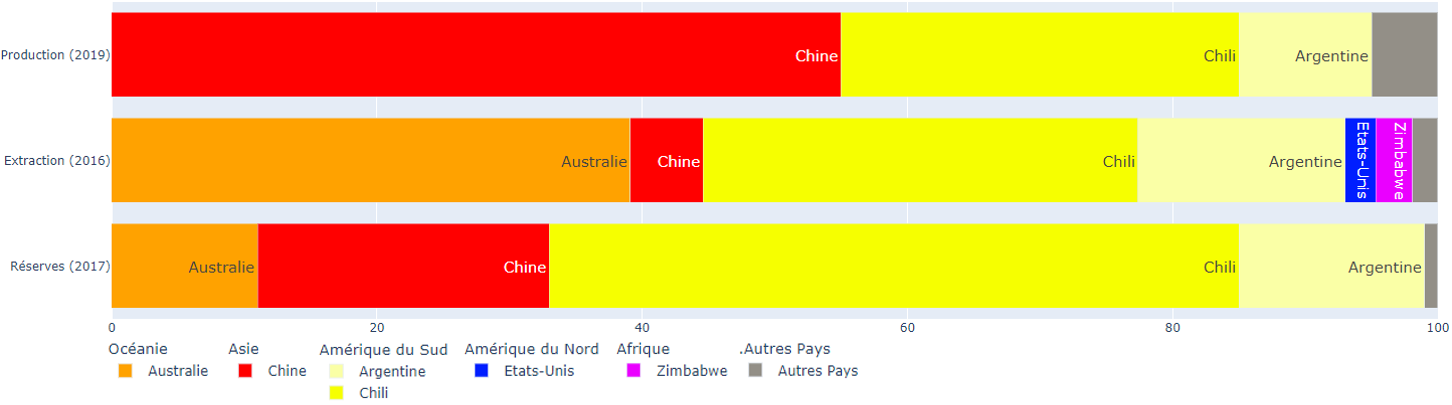
\includegraphics[width=\textwidth]{Illustration métaux/Lithium.png}

\begin{center}
    \textbf{Usage et consommation}
\end{center}
Le lithium est utilisé à 37\% pour la fabrication de batterie et à 30\%
pour la fabrication de verres et céramiques. Dans le domaine énergétique,
le lithium sert exclusivement à la fabrication de batteries.
\begin{center}
    \textbf{Prospective}
\end{center}
\begin{multicols}{2}
    \begin{center}
        \textit{Total lithium demand by sector and scenario}
    \end{center}
    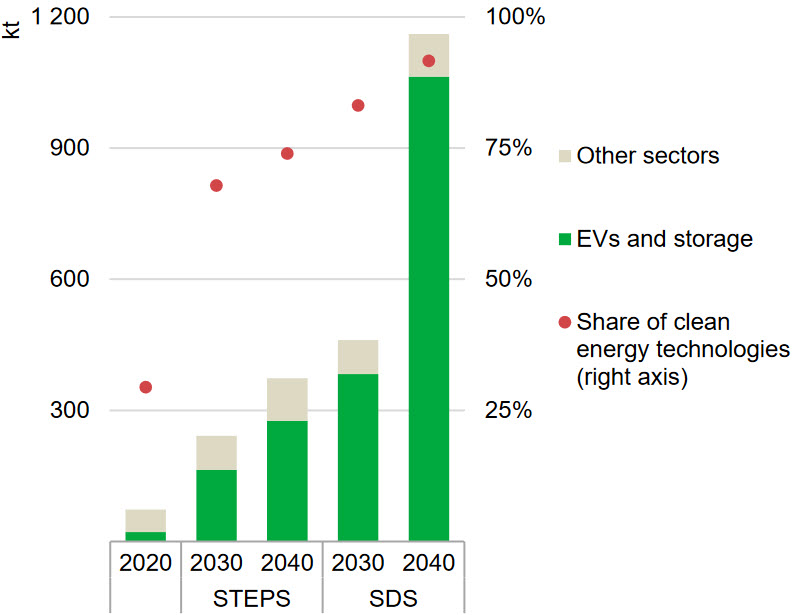
\includegraphics[width=0.45\textwidth]{Illustration métaux/lithium_prospective.jpg}
    \vfill\null
    \columnbreak
    Le lithium est le métal dont la croissance de la demande est prévue
    d'être la plus forte. Cette croissance est causée par la hausse de la
    fabrication de batteries (en majorité pour les véhicules électrique).

    \end{multicols}
\begin{center}
    \textbf{Production et recyclage}
\end{center}
La production minière de lithium a connu un taux de croissance annuel moyen
de 7,8\% entre 2001 et 2016. La production minière dépasse 36 000 kt/an. Moins de 1\% du lithium est recyclé. 
\begin{center}
    \textbf{Substituabilité}
\end{center}
Le lithium dans les batteries peut être substitué en contrepartie de baisse
de performance technologique et de hausse du coût. Les incitations à la substitution
sont faibles en raison de l'évolution technologique en faveur des batteries lithium.
\begin{center}
    \textbf{Prix}
\end{center}
Le prix du lithium est fortement volatile. Il a oscillé entre 6 et 20 US\$/kg entre
2007 et 2018. La valeur de marché de la production annuelle de lithium est de
l'ordre de 2,3 G US\$.
\clearpage
\begin{center}
    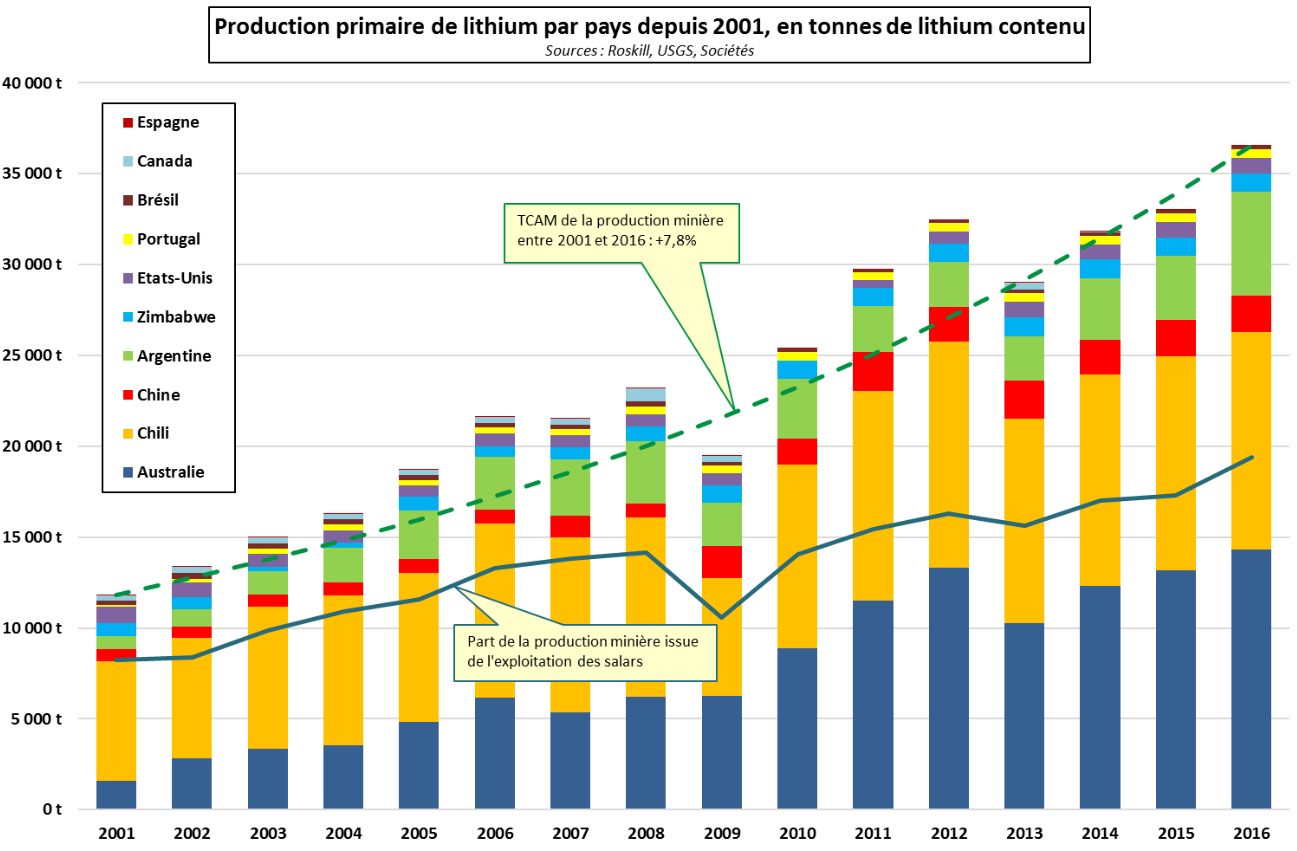
\includegraphics[width=12cm]{Illustration métaux/dynamique_lithium.png}
\end{center}
\begin{center}
    \textbf{Evènements géopolitiques}
\end{center}
Il n'y a pas eu d'évènements géopolitiques notables entre 2000 et 2020.
\begin{multicols}{2}
    \begin{center}
      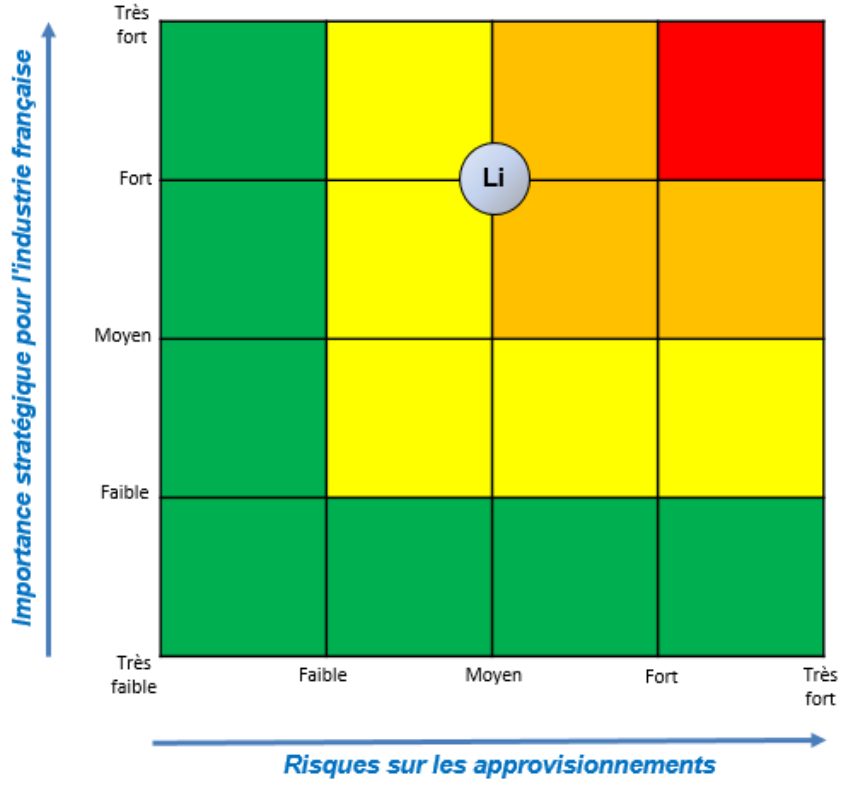
\includegraphics[width=0.35\textwidth]{Illustration métaux/Lithium_criticité.png} 
    \end{center}
    \begin{center}
    \textbf{Criticité en France}
    \end{center}
    Le risque sur les approvisionnements en lithium demeure moyen grâce à une part importante de la production minière située dans des pays de l'OCDE. Le métal reste néanmoins peu substituable et stratégique pour l'électronique et les véhicules électriques.
\end{multicols}
\begin{wrapfigure}{R}{0.65\textwidth}
  \begin{center}
    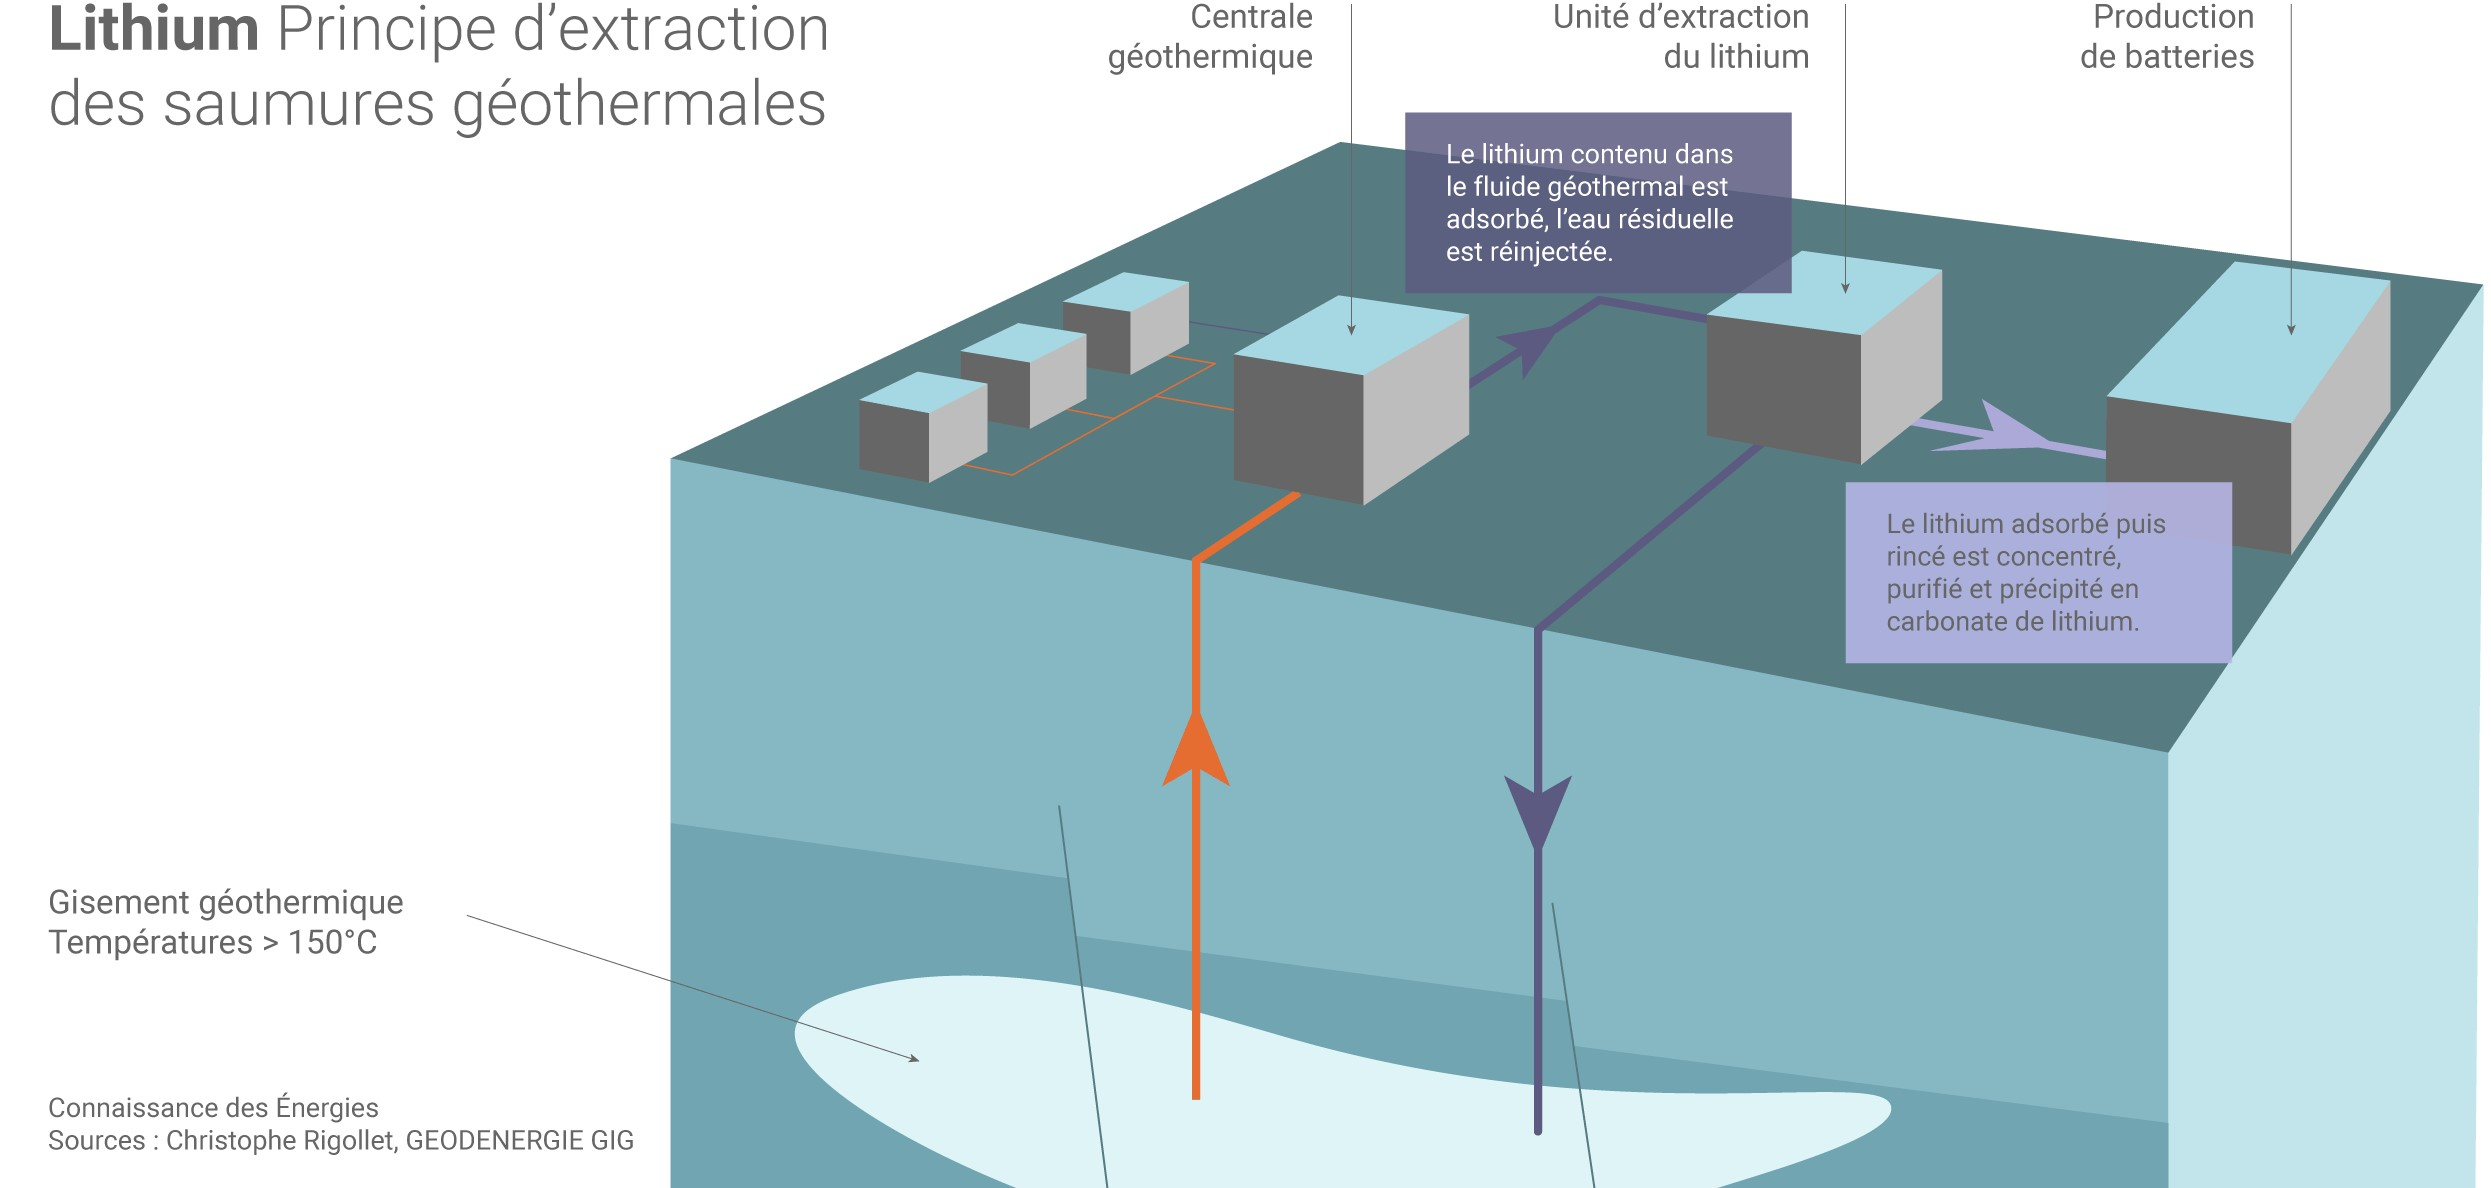
\includegraphics[width=0.65\textwidth]{Illustration métaux/extraction-lithium-geothermie-tribune-rigollet-tardieu-zoom.jpg}
  \end{center}
\end{wrapfigure}
\begin{center}
    \textbf{Opportunités}
\end{center}

L'approvisionnement en lithium comporte peu de risques spécifiques au-delà du stress hydrique sur l'approvisionnement. Des opportunités de production sont présentes en Union européenne. En Alsace, la coproduction possible de lithium est évalué à 15 000 tonnes par an sur 10 sites géothermique grâce à l'extraction du lithium des saumures. Le principe de l'extraction consiste à récupérer des eaux chaudes et riches en lithium entre 1000 et 4000 m de profondeur, d'en extraire la chaleur pour des usages énergétique et le lithium pour la production de batteries avant de remettre l'eau dans le sol.

% \begin{center}
%     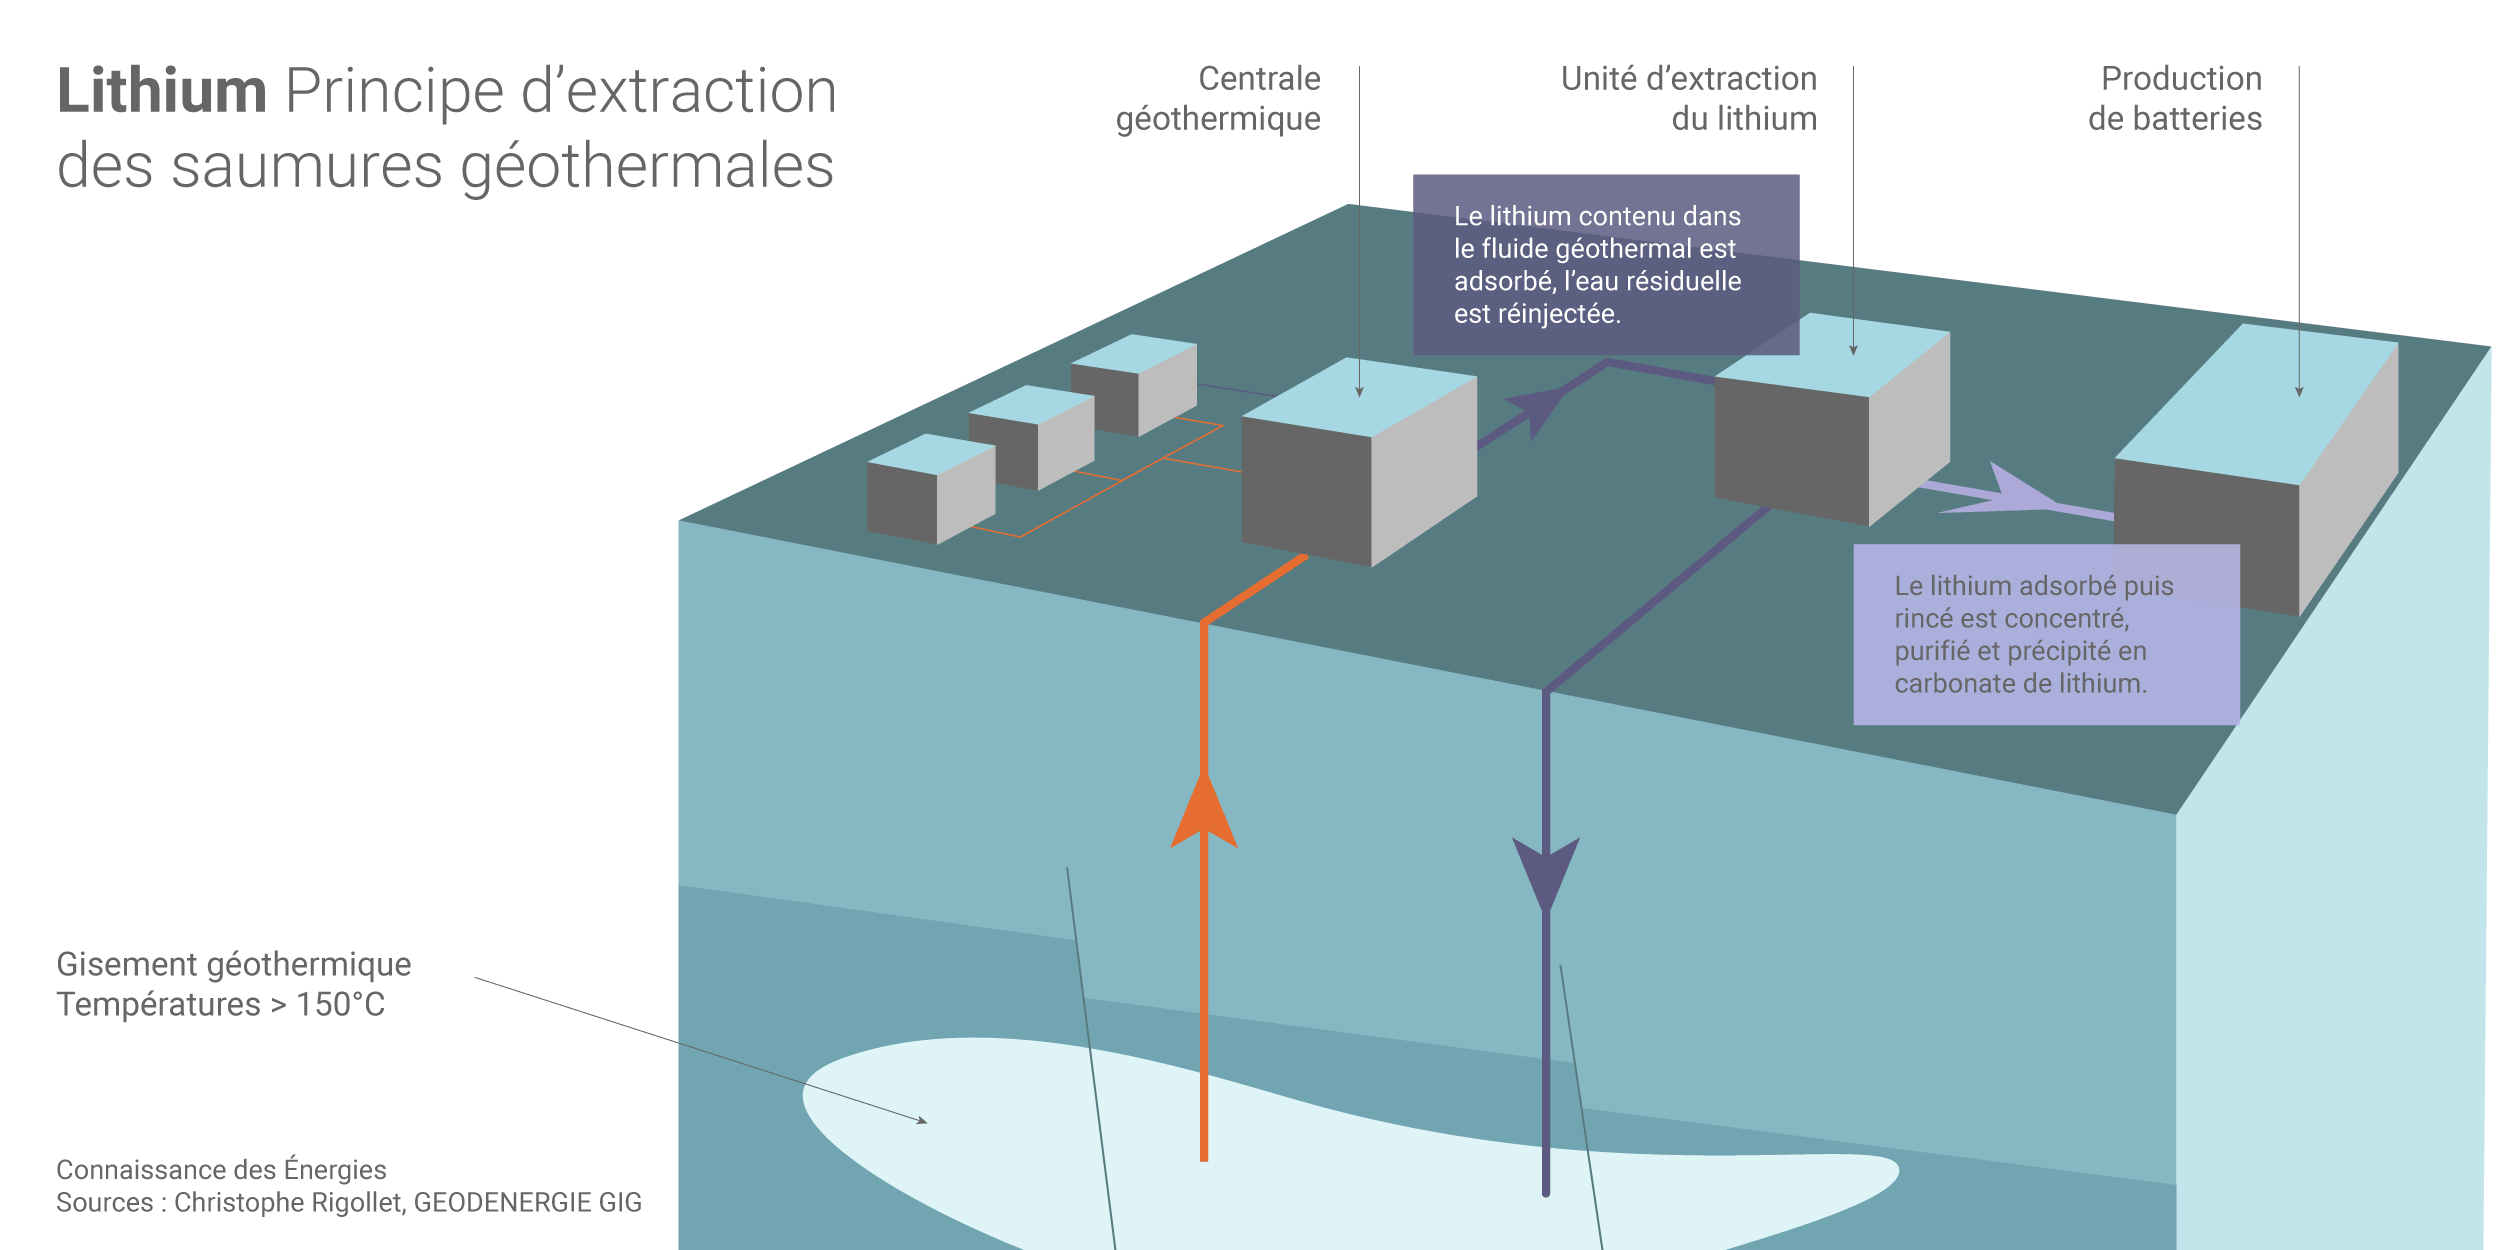
\includegraphics[width=10cm]{Illustration métaux/extraction-lithium-geothermie-tribune-rigollet-tardieu-zoom.png}
% \end{center}

\begin{center}
\subsubsection*{Cobalt}
\addcontentsline{toc}{subsubsection}{Cobalt}
\end{center}
\begin{center}
    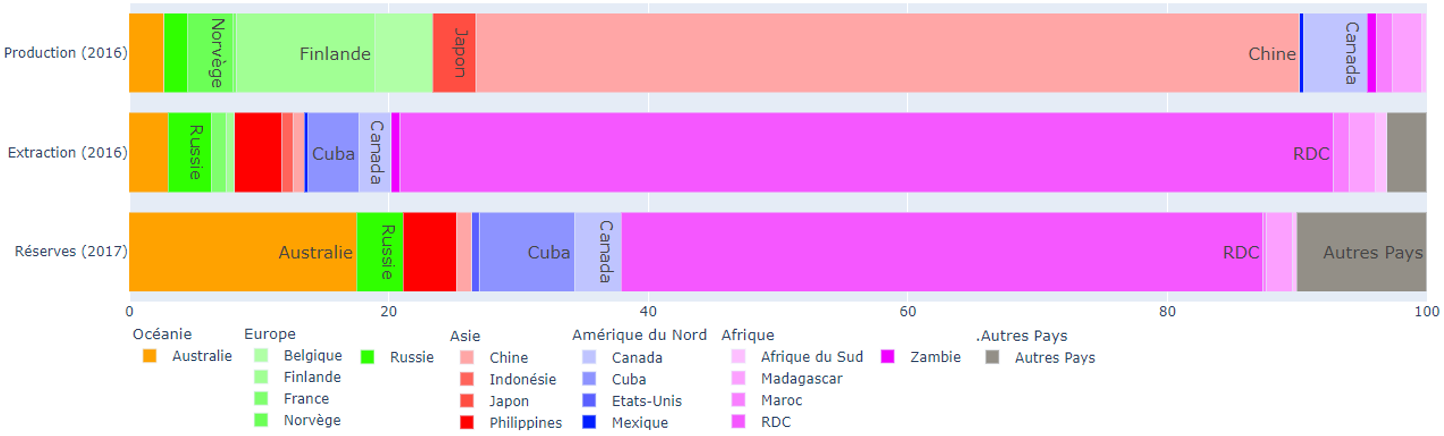
\includegraphics[width=\textwidth]{Illustration métaux/Cobalt.png}
\end{center}

\begin{center}
    \textbf{Usages et consommation}
\end{center}
La fabrication de batterie (véhicules électriques et électroniques) utilise 58\% de la production mondiale de cobalt. Le deuxième usage de cobalt est la fabrication de superalliages avec 15\%.
\begin{center}
    \textbf{Prospective}
\end{center}
\begin{multicols}{2}
    \begin{center}
        \textit{Total cobalt demand by sector and scenario}
    \end{center}
    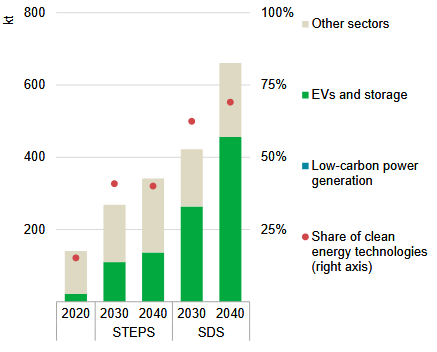
\includegraphics[width=0.45\textwidth]{Illustration métaux/Cobalt prospective.png}
    \vfill\null
    \columnbreak
    La décarbonation des activités humaines va impliquer une forte hausse de la demande en cobalt pour la fabrication des véhicules. Le taux de croissance annuel moyen de la production de cobalt raffiné a été de 7,4\% entre 2009 et 2019. 
    L'évolution de la demande en cobalt est très dépendante des choix technologiques pour les batteries suivis. 
    La chaîne d'approvisionnement en cobalt est amenée à rester concentré en Chine et en République démocratique du Congo.
    
    
\end{multicols}
\begin{center}
    \textbf{Production et recyclage}
\end{center}
Le cobalt est un métal avec une très forte concentration économique pour la production brut avec la République Démocratique du Congo et raffinée avec la Chine. Par ailleurs, la Chine influe sur de nombreux actifs de RDC \textit{via} des investissements. Le taux de recyclage du cobalt est d'environ 35\%. La production minière dépasse les 120 kt/an.
\begin{center}
    \textbf{Substituabilité}
\end{center}
Dans la fabrication des batteries, le cobalt est substituable par un changement de technologie ou par des changements de compositions chimiques.
\begin{center}
    \textbf{Prix}
\end{center}
Le prix du cobalt est volatile. Le prix moyen est de 31 176 US\$/t en 2020. Avec une valeur du marché dépassant les 4.3 G US\$.
\clearpage
\begin{center}
    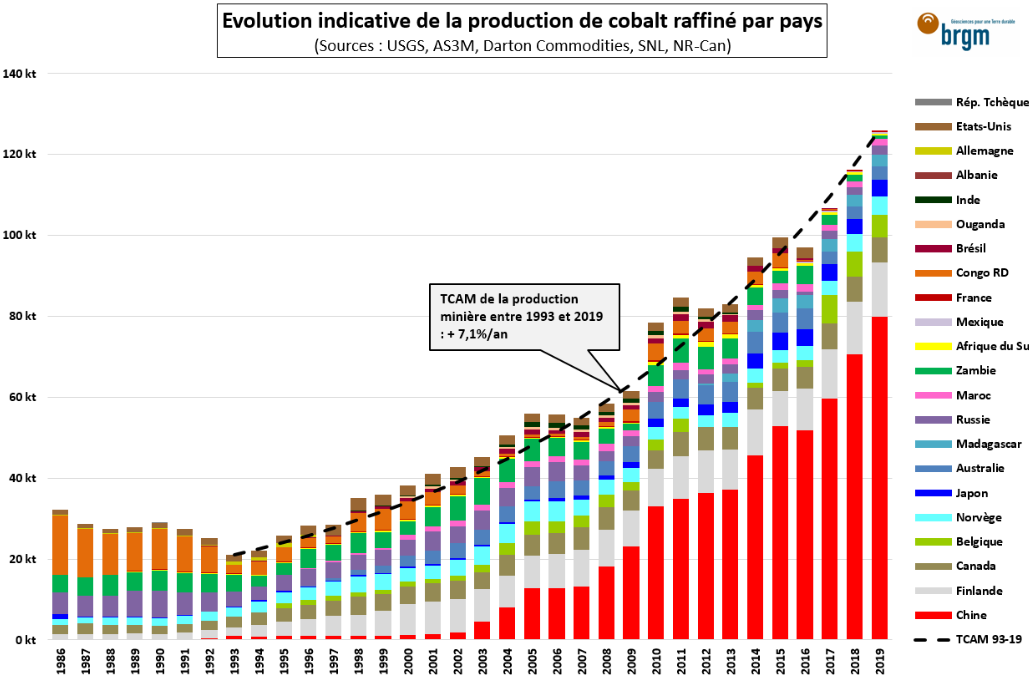
\includegraphics[width=12cm]{Illustration métaux/dynamique_cobalt.png}
\end{center}
\begin{center}
    \textbf{Evènements géopolitiques}
\end{center}
Des perturbations d'approvisionnement locales ont été recensées. En 2015, le site de production de Chambishi a été perturbé par des tension avec la RDC, entraînant des suspensions dans l'approvisionnement par ce site. En 2007, des différends politiques ont perturbé l'approvisionnement en cobalt par la RDC pendant près d'un an entrainant des augmentations de prix. (\cite{hatayama_adopting_2018})

\begin{multicols}{2}
    \begin{center}
      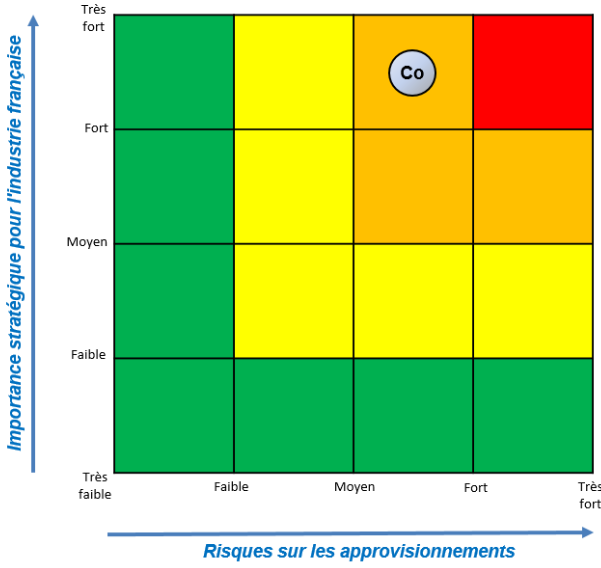
\includegraphics[width=0.35\textwidth]{Illustration métaux/Cobalt_criticité.png} 
    \end{center}
    \begin{center}
    \textbf{Criticité en France}
    \end{center}
    Le cobalt est particulièrement important pour l'industrie du fait des nombreux secteurs d'usages comme l'énergie, l'aéronautique, la défense et l'autombile. La forte concentration du marché engendre un risque sur l'approvisionnement important.
\end{multicols}

\begin{center}
    \textbf{Risques spécifiques}
\end{center}
Une part significative de la production minière de cobalt est issue de petites mines artisanales, bien que ces mines permettent de stabiliser les prix de marché grâce à leur production flexible. La fiabilité de l'approvisionnement par ces mines est affaiblie par les vulnérabilités sociales et économiques de ces sites de production. Ces petites mines artisanales sont particulièrement peu régulées incluant des conditions de travail dangereuses et la présence de travail des enfants.\\
Le cobalt est souvent un sous-produit du cuivre et du nickel. En conséquence, il est possible qu'il n'y ait pas d'investissements dans la production de cobalt tant que le marché du cuivre et du nickel n'envoient pas de signaux pour investir dans la production.
\begin{center}
\subsubsection*{Terres Rares}
\addcontentsline{toc}{subsubsection}{Terres Rares}
\end{center}
\begin{center}
    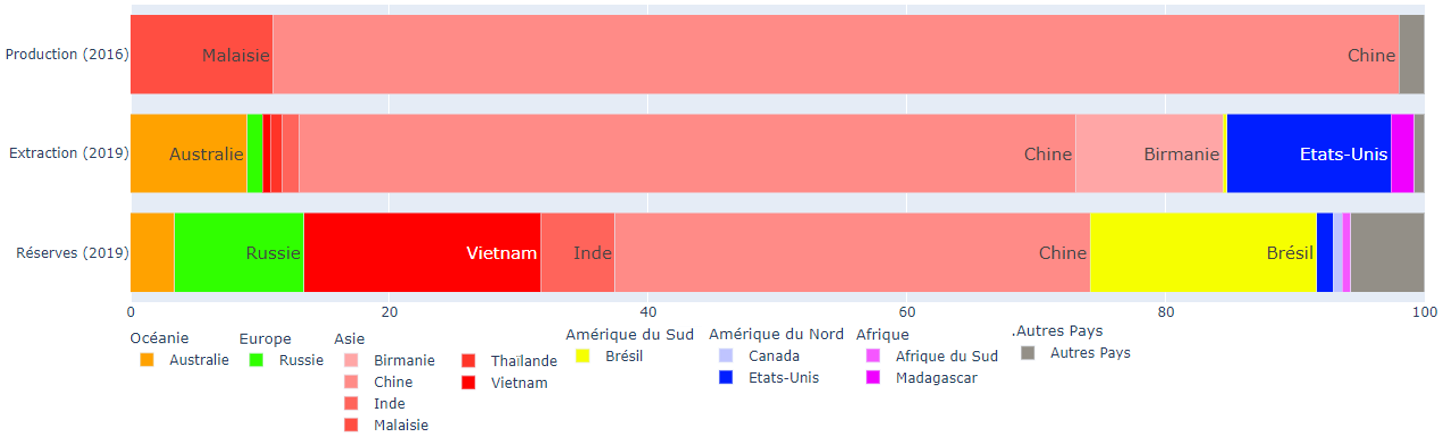
\includegraphics[width=\textwidth]{Illustration métaux/TR.png}
\end{center}
\begin{center}
    \textbf{Définition}
\end{center}
Les terres rares sont un groupe de métaux aux propriétés voisines comprenant le néodyme, le dysprosium, l'yttrium...\\

\begin{center}
    \textbf{Usages et consommation}
\end{center}
La demande en terres rares est particulièrement tirée par la fabrication
d'aimants permanents. Les aimants permanents sont fortement utilisés dans
le domaine de l'énergie pour la fabrication de génératrices (éoliennes en mer)
et de moteurs électriques (véhicules électriques).
\begin{center}
    \textbf{Prospective}
\end{center}
\begin{multicols}{2}
    \begin{center}
        \textit{Total RRE demand by sector and scenario}
    \end{center}
    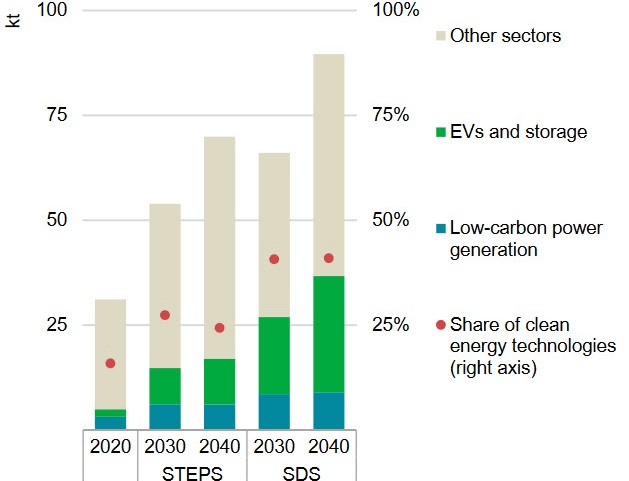
\includegraphics[width=0.45\textwidth]{Illustration métaux/RRE_prospective.jpg}
    \vfill\null
    \columnbreak
Il est prévu que la demande mondiale en terres rares augmente en partie à cause
de la décarbonation du mix énergétique mondial. La décarbonation du mix
énergétique mondial stimule la demande en majorité par le besoin en véhicule électrique
et sur un second plan par la construction de moyens de production bas-carbone.
Des projets miniers sont en développement sur tous les continents.
\end{multicols}
\begin{center}
    \textbf{Production et recyclage}
\end{center}
Le taux de croissance annuel moyen de la production minière de terres rares est entre 3 et 4\%. La production minière dépasse 150 kt/an. Le monopole de la Chine est en train de se réduire pour la production minière avec une production minière estimée à 57\% en 2020, contre plus de 95\% en 2011, grâce à de nouvelles productions en Birmanie ou aux Etats-Unis.
\begin{center}
    \textbf{Substituabilité}
\end{center}
Les terres rares ne peuvent pas être substituées sans pertes de performances
techniques pour la fabrication d'aimants permanents. 

\begin{center}
    \textbf{Prix}
\end{center}
Le prix des terres rares ont connu des épisodes de forte volatilité.
Le prix est d'environ 290 US\$/kg pour le dysprosium (2016) et et 50\$/kg pour le neodyme (2015).
\clearpage
\begin{center}
    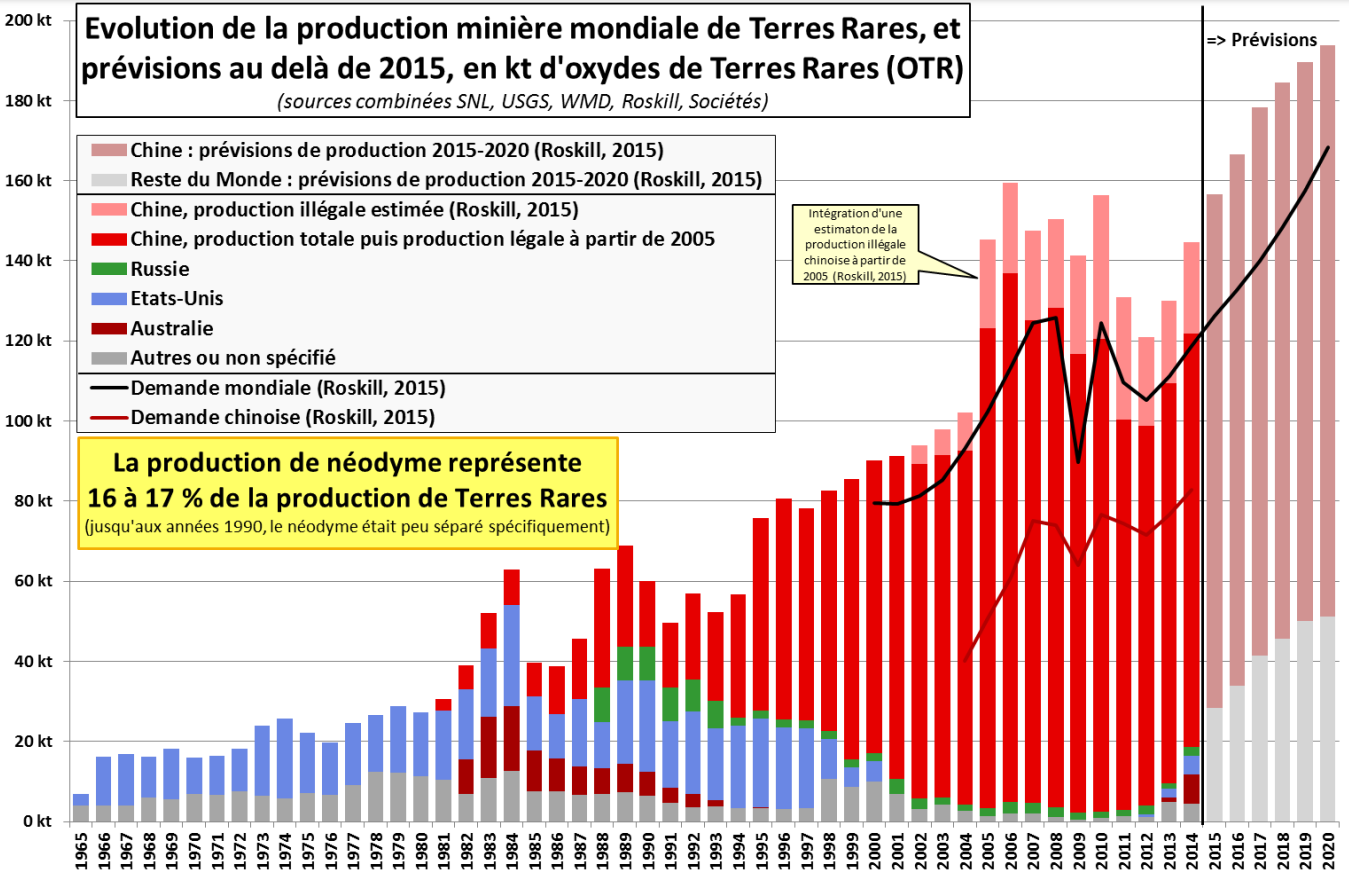
\includegraphics[width=12cm]{Illustration métaux/Dynamique_TR.png}
\end{center}
\begin{center}
    \textbf{Evènements géopolitiques}
\end{center}
La Chine a accéléré la limitation des exportations de terres rares en 2011 (voir encadré \hyperref[Chine]{\textit{Les terres rares chinoises : une arme  économique et géopolitique}})
\begin{multicols}{2}
    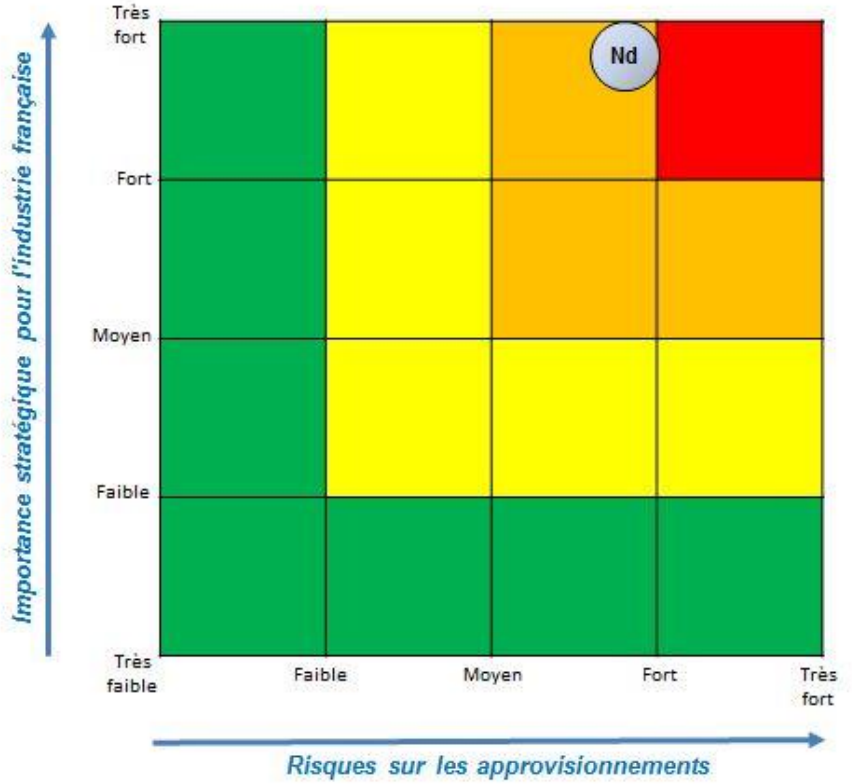
\includegraphics[width=0.35\textwidth]{Illustration métaux/TR_criticité.png}
    \begin{center}
    \textbf{Criticité en France}
    \end{center}
    Le risque sur les approvisionnements en terres rares est fort pour toutes les terres rares. Cependant l'impact stratégique sur l'industrie varie selon les terres rares. Pour le secteur énergétique, le néodyme est particulièrement stratégique pour la fabrication d'aimants permanents.
\end{multicols}
\begin{center}
    \textbf{Risques spécifiques}
\end{center}
Bien que la production minière se soit diversifiée, le raffinage reste dominé par la Chine. Il y a actuellement quatre unités de raffinage en dehors de Chine, en Malaisie, en Inde, en Estonie et en France.\\

\begin{center}
    \boxput*(0,1){
        \colorbox{white}{Terres rares en France}
    }{
    \setlength{\fboxsep}{15pt}
    \fbox{\begin{minipage}{14cm} 
    L'usine Solvay de La Rochelle a été fondée en 1948. A l’origine, le site fabriquait des pierres à briquets. Aujourd’hui, l’usine a une expertise reconnue dans la séparation et la purification des Terres Rares et la fabrication de produits de haute technologie servant les marchés de la dépollution automobile, de l’imagerie médicale et du polissage pour l’électronique et pour les verres de haute précision.\\
    Elle produit chaque année environ 4 000 tonnes de produits de formulation à base de terres rares pour les marchés de la catalyse, de la dépollution automobile, du polissage et de l’électronique (\cite{solvay_rochelle_2022})
    \end{minipage}}.
    }
\end{center}


\clearpage
\subsection{Comparaison avec le pétrole}
\label{section:comparaison}
\subsubsection{Analyse quantitative}
\textbf{Méthodologie}
\smallbreak
D'abord, nous avons évalué la concentration des réserves et de la production du cuivre, du nickel, du lithium, du cobalt, des terres rares et du pétrole, bruts et raffinés. Ainsi, nous avons calculé l'indice Herfindal-Hirschman (HHI) pour chacun d'eux. La formule de cet indice est la suivante :
$$
HHI = \sum_{i=1}^n s_i^2
$$
Avec $n$ le nombre le pays producteurs, et $\forall i \in [1,...,n]$, $s_i$ est la part du pays $i$ dans la production, l'extraction de ressource brute et la production de ressource raffinée. Un HHI situé entre 0 et 1500 dénote une concentration faible, modérée s'il est entre 1500 et 2500, et au-delà, le secteur sera considéré comme hautement concentré.
\smallbreak
Les données utilisées sont tirées des fiches synthèses du BRGM sur la criticité des métaux (\cite{brgm_fiche_2016}),(\cite{brgm_fiche_2016-1}),(\cite{brgm_fiche_2017}),(\cite{brgm_fiche_2018}),(\cite{brgm_fiche_2021}), et du rapport \textit{bp Statistical Review of World Energy} (\cite{bp_statistical_2022}). Pour le pétrole, les données comprennent le pétrole brut, le pétrole de schiste, les sables bitumineux, les condensats (condensats de location ou condensats de gaz qui nécessitent un raffinage supplémentaire) et les LGN (liquides de gaz naturel - éthane, GPL et naphte séparés de la production de gaz naturel).
 En revanche, elles ne comprennent pas les combustibles liquides provenant d'autres sources, comme les biocarburants et les dérivés synthétiques du charbon et du gaz naturel. Sont également exclus les facteurs d'ajustement des combustibles liquides tels que le gain de traitement en raffinerie. Elles excluent également les schistes bitumineux/kérogène extraits sous forme solide.
 Il convient de préciser que les années de référence peuvent différer car les estimations des ressources et de la production des métaux étudiés ne sont pas conduites chaque année. Celles-ci varient donc entre 2016 et 2019 (voir figure \ref{fig:HHI}).
\smallbreak
Ensuite, nous avons comparé le pétrole et les métaux stratégiques susnommés sous l'angle de la stabilité politique. En effet, l'instabilité politique peut être un facteur majeur de conflits, d'accaparation des ressources et autres risques pesant sur la chaîne d'approvisionnement. Pour ce faire, la moyenne de l'indicateur "Stabilité politique et absence de violence/terrorisme" déterminé par la Banque Mondiale a été calculée en la pondérant par la part de chaque pays dans la production et l'extraction. La Banque mondiale définit cet indicateur comme la perception de la probabilité d'instabilité politique et/ou de violence à motivation politique, y compris le terrorisme. Cela prend la forme d'une note entre environ -2,5 et 2,5, la moyenne pour tous les pays du monde étant égale à 0 (voir figure \ref{fig:Polit World Bank}). Ainsi, on peut considérer comme "bon" un score supérieur à 0, et mauvais s'il est inférieur à 0.

\bigbreak
\textbf{Résultats et interprétations}
\smallbreak
\begin{figure}
    \centering
    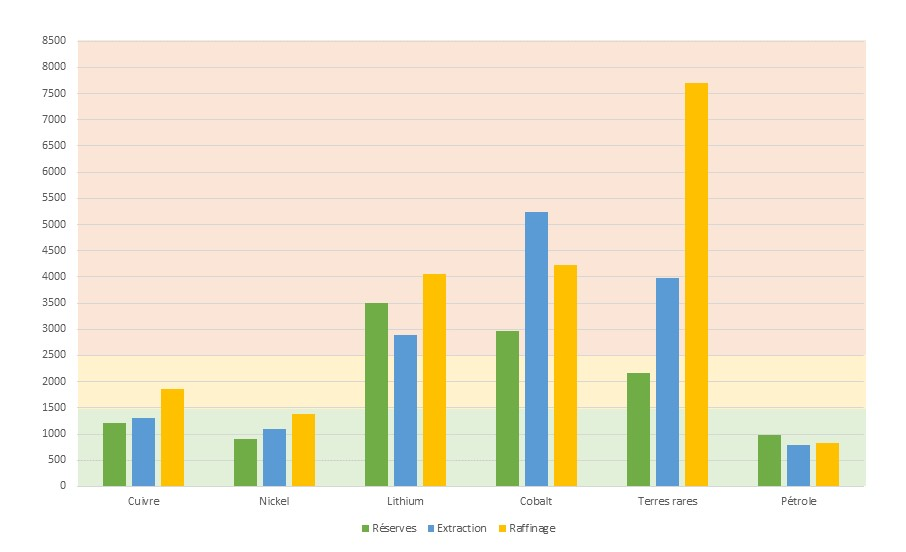
\includegraphics[width=0.8\textwidth]{Images/02 appro/graphe hhi.jpg}
    \caption{Indice Herfindahl-Hirschman des pays extrayant les minerais étudiés et du pétrole. Données tirées de section \ref{section:fiches} ,(\cite{bp_statistical_2022})}
    \label{fig:HHI}
\end{figure}

Sur ce graphe, seuls le pétrole et le nickel ont des réserves, une extraction et une production peu concentrées. Les réserves et l'extraction de cuivre sont peu concentrées, mais sa production l'est modérément. Les autres métaux étudiés ont tous une concentration élevée pour les trois variables, à l'exception des terres rares. En ce qui concerne ces dernières, leur présence géologique dans l'ensemble de la croûte terrestre explique que leurs réserves ne soient que modérément concentrées. Cependant, leur raffinage est particulièrement concentré, tiré par le poids de la Chine malgré une progressive diversification depuis 2010 (voir \hyperref[Chine]{\textit{Les terres rares chinoises : une arme  économique et géopolitique}}). Le HHI bien moins élevé pour le secteur pétrolier que celui des autres ressources étudiées doit cependant être mis en perspective avec le fait que les pays producteurs de pétrole sont géographiquement proches. D'autant plus que la valeur économique des marchés mondiaux de ces métaux est bien moins élevée que celle du marché du pétrole \cite{manberger_geopolitics_2019}.
\smallbreak
Si le cuivre apparaît moins concentré, il faut toutefois souligner que les secteurs qui en dépendent sont nombreux, rendant plus importantes les conséquences industrielles d'une éventuelle rupture d'approvisionnement. Au contraire, les volumes de production bien moindres du cobalt et des terres rares minimisent ces dernières. Le lithium, produits en gros volumes, est plus concentré en comparaison du cuivre, mais des pays de l'OCDE comme le Canada, l'Australie ou encore la France font partie des principaux extracteurs, diminuant de ce fait le risque d'approvisionnement (\cite{brgm_fiche_2017}). 

\begin{figure}
    \centering
    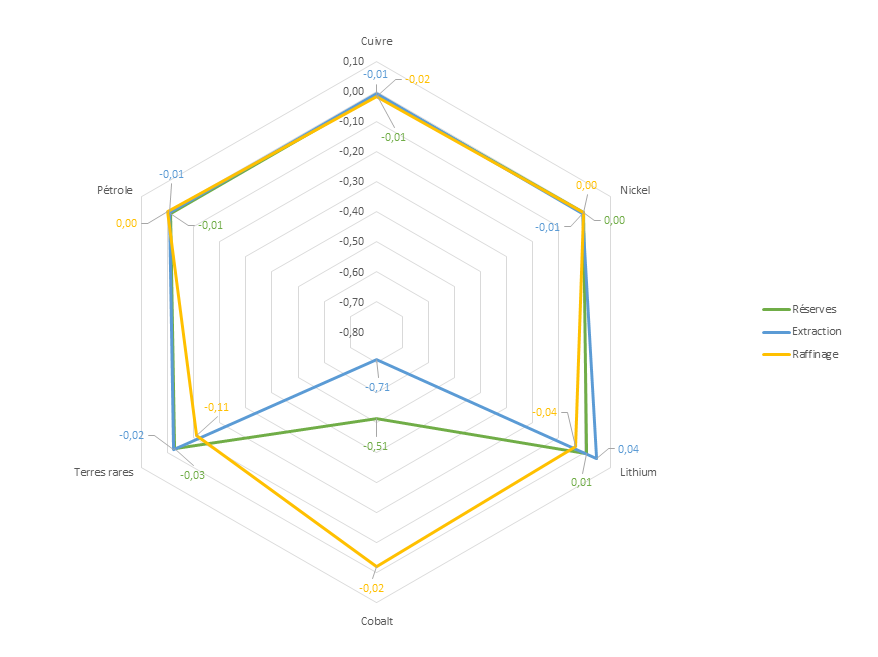
\includegraphics[width=0.8\textwidth]{Images/02 appro/graphe gouvernance.png}
    \caption{Moyenne de l'indice de stabilité politique pondéré par la part de chaque pays dans la production et les réserves de la ressource étudiée. Données tirées de (\cite{world_bank_wgi_2023})}
    \label{fig:Polit World Bank}
\end{figure}
On ne peut pas déduire du calcul de la moyenne de l'indice de stabilité politique que le secteur pétrolier soit plus ou moins vulnérable à l'instabilité et aux violences que ceux du cuivre et du nickel. Toutefois, le score du pétrole tend plus vers la moyenne mondiale que celui des terres rares, du cobalt et du lithium. Une tendance générale est que le secteur du raffinage est moins soumis à l'intabilité, à l'exception des terres rares. Cela peut être expliqué par le fait que les démocraties libérales, mieux notées sur cet indicateur par la Banque mondiale que les régimes autoritaires, ont développé des capacités de raffinage, alors que la transformation des terres rares est toujours dominée par la Chine. La bonne moyenne obtenue par le secteur de la production de lithium brut s'explique par le fait que l'Australie est un acteur majeur de celle-ci, tandis que pour le raffinage la Chine tire le score vers le bas. Quant au cobalt, les scores des réserves et de la production sont si bas en raison la prépondérance de la République Démocratique du Congo. En effet, le pays se relève à peine de la résurgence d'un conflit armé dans les régions de l'Est, qui ont favorisé l'essor du terrorisme. La présence de ressources en cobalt a d'ailleurs pu aggraver ces violences, dans la mesure où ce minéral combine une valeur élevée par poids et volume et la possibilité d'une exploitation minière artisanale (\cite{manberger_geopolitics_2019}).
\smallbreak
\smallbreak
\textbf{Limites et biais}
\smallbreak
Premièrement, la concentration d'un secteur n'est pas nécessairement synonyme de tensions sur la chaîne d'approvisionnement. Un métal peut être très concentré géographiquement mais être produit par des pays qui sont moins susceptibles d'aller à l'encontre des règles du commerce international en perturbant la production ou les exportations de ressources pour leur intérêt national. De plus, les limites entre ce qui est considéré comme peu, modérément et très concentré peuvent être interrogées.
\smallbreak
C'est pourquoi nous avons voulu examiner également l'indice de stabilité pondéré par le poids des pays dans les réserves, la production et l'extraction. Mais cet outil est aussi incomplet. Par définition, étant une moyenne, il est tiré par la note des pays les plus importants dans les réserves et la production. De plus, les indicateurs de la Banque Mondiale sont fondés sur des perceptions d'experts et des populations. La dimension subjective de celle-ci doit donc être prise en compte.
\smallbreak
(\cite{hache_vers_2019}) soulignent d'ailleurs des lacunes dans l'évaluation de la dimension géopolitique de la criticité, dans la prise en compte de l'évolution des restrictions aux importations et dans les recherches empiriques sur le lien entre instabilité politique et disruption des chaînes d'approvisionnement.

\subsubsection{Conséquences en cas de rupture d'approvisionnement}
Au premier abord, les usages captifs du pétrole et des métaux critiques diffèrent de telle sorte que les économies sont plus sensibles à une pénurie ou à une hausse des prix du premier. Une éventuelle crise des approvisionnement pétroliers affecte en premier lieu le secteur des transports, dont sont dépendants non seulement le fret mais également les particuliers. En revanche, une crise affectant un métal contenu dans les batteries de voitures électriques ou des panneaux solaires n'aura pas de conséquence sur les usagers finaux de ces équipements (\cite{iea_role_2021}).
\smallbreak
De même, le secteur de la pétrochimie, qui est le deuxième secteur le plus consommateur de pétrole avec 14\% des consommations totales en 2017, est indispensable aux modes de vie modernes et à la sécurité alimentaire. Il produit notamment les plastiques qui sont le groupe de matériaux en vrac à la croissance la plus rapide du monde. De ce secteur découlent également les engrais azotés de synthèse, qui sous-tendent près de la moitié de la production agricole mondiale (\cite{iea_future_2018}). 
\smallbreak
Une autre différence majeure entre le pétrole et les métaux est que le premier est définitivement brûlé quand il est utilisé, alors que les seconds restent présents dans les infrastructures et les équipements. Cela implique une potentielle récupération et réutilisation grâce au recyclage en fin de vie (voir section \ref{section:maitrise_techno}).
\smallbreak
Ainsi, des disruptions dans les chaînes d'approvisionnement des métaux de la transition énergétique supposeront que celle-ci sera retardée et plus coûteuse, mais elles n'affecteront pas directement les vies quotidiennes des consommateurs (\cite{iea_role_2021}). Néanmoins, elles peuvent constituer de lourdes perturbations sur les industries, et donc entraîner des ralentissements des économies. Par exemple, la mise en place par la Chine de quotas d'exportations de terres rares, suivie d'un embargo non-officiel à l'encontre du Japon (voir encadré \hyperref[Chine]{\textit{Les terres rares chinoises : une arme économique et géopolitique}}), a eu des conséquences sur l'industrie automobile nippone. En septembre 2011, l'entreprise Toyota a annoncé envisager de transférer la fabrication de certains modèles de véhicules hybrides vers la Chine pour éviter lesdits quotas (\cite{niquet_chine_2011}). Cela revêt une importance stratégique dans la course aux brevets pour les technologies bas-carbone et au leadership dans ce secteur.
\smallbreak
Par ailleurs, le pétrole et les minéraux ont en commun que des menaces sur la fiabilité d'approvisionnement peuvent considérablement se répercuter sur les systèmes énergétiques. Dès lors, les préoccupations autour de la sécurité pétrolière sont applicables aux matériaux critiques. Dès lors, la sécurité minérale peut être fondée sur l'expérience retirée des marchés pétroliers. En particulier, comme ce fut le cas pour la sécurité pétrolière, il faut accompagner les mesures sur l'offre d'efforts sur la demande et la résilience : usage de matériaux recyclés, promouvoir une utilisation efficace, évaluer la robustesse des chaîne d'approvisionnement... (voir sections \ref{section:levier} et \ref{section:politiques_publiques}) (\cite{iea_role_2021}).
\bigbreak

\begin{center}
    \boxput*(0,1){
        \colorbox{white}{Les terres rares chinoises : une arme économique et géopolitique}
    }{
    \setlength{\fboxsep}{15pt}
    \fbox{\begin{minipage}{14cm} 

    
« Il y a le pétrole au Moyen-Orient, il y a des terres rares en Chine », aurait dit Deng Xiaoping, initiateur des réformes d’ouverture de l’économie chinoise. Cette citation a un aspect presque prémonitoire, car bien que cela ait évolué depuis (voir section 2.1), en 2011, la République populaire de Chine (RPC) concentrait 50\% des réserves connues et 97,3\% de la production, grâce à son atout-prix. Sa position quasi-monopolistique dans la production de terres rares lui a d’ailleurs servi comme une arme afin d’arriver à ses fins géopolitiques.  \smallbreak
En 2010, un chalutier de pêche chinois et deux bateaux de patrouille des garde-côtes japonais sont entrés en collision en mer de Chine orientale, précisément dans les zones maritimes disputées autour des îles Senkoku/Diaoyu. Cet accrochage a provoqué le contrôle du bâtiment chinois, puis l’emprisonnement de son capitaine au Japon. Suite à cela, la Chine a graduellement réduit ses exportations de terres rares vers le Japon, qui en était alors fortement dépendant : en 2011, 81\% des importations japonaises de ces minerais provenaient de RPC. Celle-ci a nié tout embargo, de façon à éviter une condamnation de l’Organisation Mondiale du Commerce (OMC).  \smallbreak
Cet événement est à mettre en parallèle avec la stratégie chinoise de restriction des exportations de terres rares progressivement mise en place durant les années 2000. En effet, en 2004, la Chine a mis en place de quotas d’exploitation sur les terres rares, de telle sorte qu’en 2006, ses exportations de ces minerais furent divisées par deux. De 2011 à 2012, elle gela officiellement les licences de prospection et d’exploitation. Ces politiques servaient les ambitions de puissances chinoises, car elles permettaient un renforcement du contrôle sur les entreprises étrangères et une promotion des entreprises d’Etat, allant dans le sens du rééquilibrage de la croissance de la RPC vers une industrie à plus forte valeur ajoutée. Cela lui a valu une condamnation par l’OMC en 2014 pour violation des règles du commerce mondiale, à la suite d’une plainte déposée en 2012 par le Japon, les Etats-Unis et l’Union Européenne.  \\
Ces épisodes ont remis au goût du jour la question de la criticité des matériaux dans la stratégie des Etats, et ont renforcé les clivages autour de l’émergence de la puissance chinoise. De ce fait, les pays qui lui étaient dépendants, notamment le Japon, ont depuis développé des contre-stratégies de contournement, par exemple en cherchant d’autres fournisseurs, en constituant des stocks stratégiques ou encore en finançant la recherche. 
\\[0.5cm]
\textit{Sources : \cite{niquet_chine_2011},\cite{lincot_terres_2021},\cite{faujas_matieres_2014}}

    \end{minipage}}
    }
\end{center}
\label{Chine}
~\\

\clearpage
\subsection{Etapes de la chaîne d'approvisionnement}
\label{section:chaine}
La figure \ref{fig:supply} récapitule la chaîne d'approvisionnement de certaines technologies bas carbone qui utilisent les matériaux que nous avons étudiés dans la sous-section précédente. Elle met en évidence le fait que la Chine est présente sur l'ensemble de la chaîne, ce qui peut lui procurer une forme de suprématie économique et la mettre en bonne voix pour asseoir un leadership sur le secteur des technologies de la transition énergétique. 
\smallbreak
En ce qui concerne l'amont de la chaîne, le raffinage apporte plus de valeur ajoutée et des emplois plus qualifiés que l'extraction. Cela peut amener des pays détenteurs de réserves à développer des capacités de transformation afin de ne pas tomber dans la malédiction des ressources, ainsi que pour avoir plus de poids face aux puissances dépendantes d'importations de métaux, comme les Etats-Unis et l'Union européenne. C'est notamment le cas en Indonésie, qui a décrété à plusieurs reprises des embargos sur ses exportations de minerais bruts (voir encadré \hyperref[Indonesia]{\textit{L'Indonésie et le nickel : existe-t-il un risque de cartellisation ?}}).
\smallbreak
Face aux risques de ruptures d'approvisionnement, en plus de la diversification des fournisseurs, les pays dépendants de ces métaux pour leur transition énergétique peuvent trouver un intérêt à relocaliser l'amont de la chaîne. De plus, avoir la main sur l'ensemble des étapes implique plus de visibilité et de transparence sur le respect des normes environnementales et le droit du travail. Seulement, du fait de plus faibles réserves, seuls de petits volumes de production pourraient être tirés de ces mines et raffineries relocalisées. Cela, de même que les normes environnementales et humaines plus sévères, rendent ces solutions peu compétitives et tributaires de prix hauts pour être rentables. Par exemple, à la suite de l'embargo non-officiel de la Chine sur les terres rares (voir encadré \hyperref[Chine]{\textit{Les terres rares chinoises : une arme économique et géopolitique}}), les Etats-Unis ont fait rouvrir la mine de Mountain Pass en 2012. Mais la prépondérance de la RPC dans ce secteur lui a permis de faire jouer les prix des terres rares à la baisse, entraînant une perte de valeur de 20\% pour les actions de Mollycorp, l'entreprise alors propriétaire du site (\cite{niquet_chine_2011}). Cette dernière a déposé bilan en 2015 (\cite{hsu_molycorp_2015}).

\begin{figure}[!b]
    \centering
    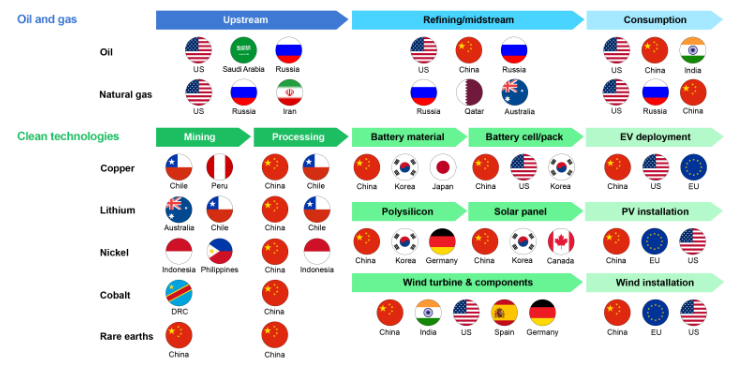
\includegraphics[width=0.8\textwidth]{Images/02 appro/SC metaux.png}
    \caption{Chaînes d'approvisionnement indicatives du pétrole et du gaz et de certaines technologies d'énergie propre. Source : \cite{iea_role_2021}}
    \label{fig:supply}
\end{figure}

\begin{center}
    \boxput*(0,1){
        \colorbox{white}{L'Indonésie et le nickel : existe-t-il un risque de cartellisation ?}
    }{
    \setlength{\fboxsep}{15pt}
    \fbox{\begin{minipage}{14cm} 
L'Indonésie a, à plusieurs reprises, mis en place des politiques d'interdiction d'exportation de minerais non transformés. La première a eu lieu entre 2014 et 2017, et la seconde a commencé en 2020 et se poursuit aujourd'hui. Cette dernière concerne pour l'instant seulement le nickel brut, mais le président Jokowi a annoncé sa possible extension à la bauxite, l'étain et le cuivre. Pour cet embargo, l'Organisation Mondiale du Commerce a condamné l'Indonésie fin 2022 à la suite d'une plainte de l'Union européenne, décision contre laquelle le pays asiatique compte faire appel.\smallbreak
L'objectif derrière ces politiques est d'encourager les investissements directs étrangers vers des fonderies ou des usines de raffinage sur le sol indonésien. Ainsi, le pays espère capter plus de valeur ajoutée, et créer plus d'emplois locaux. Mais ces embargos successifs ont également encouragé les investissements dans les projets miniers dans d'autres pays, ce qui pourrait affaiblir la position de l'Indonésie sur le long terme.\smallbreak
Au-delà des considérations économiques, les restrictions indiquent aussi une volonté géopolitique d'affichage de puissance : il s'agit ici de montrer que le pays a la capacité d'influence pour disrupter le cours du nickel. Cela s'est en outre traduit par une déclaration faite par le ministre de l’Investissement Bahlil Lahadalia dans le Financial Times en octobre 2022 : l'Indonésie étudie la possibilité de créer un cartel, similaire à l'Organisation des Pays Producteurs de Pétrole (OPEP), pour les principaux producteurs de métaux des batteries.\smallbreak
Seulement, on peut s'interroger sur la vraisemblance du risque de cartellisation pour les métaux. Si l'OPEP a une telle importance géopolitique, c'est notamment grâce à la vague de nationalisation de la production pétrolière par ses pays fondateurs, qui a transféré le pouvoir d'influence des majors vers les gouvernements. Or, dans le cas du nickel, rien qu'en Indonésie, pourtant porteuse de l'initiative, les entreprises étrangères constituent une grande part de la production, dont la brésilienne Vale qui est même un des acteurs majeurs du secteur minier indonésien.

\textit{Sources : \cite{hache_metaux_2022},\cite{strangio_indonesia_2022}}

    \end{minipage}}
    }
\end{center}
\label{Indonesia}
~\\
\clearpage
\printbibliography
\clearpage
% 3
\clearpage
\begin{refsection}
\section{Maîtrise technologique et industrielle}
    \begin{figure}[!b]
\centering
\begin{subfigure}{0.4\textwidth}
    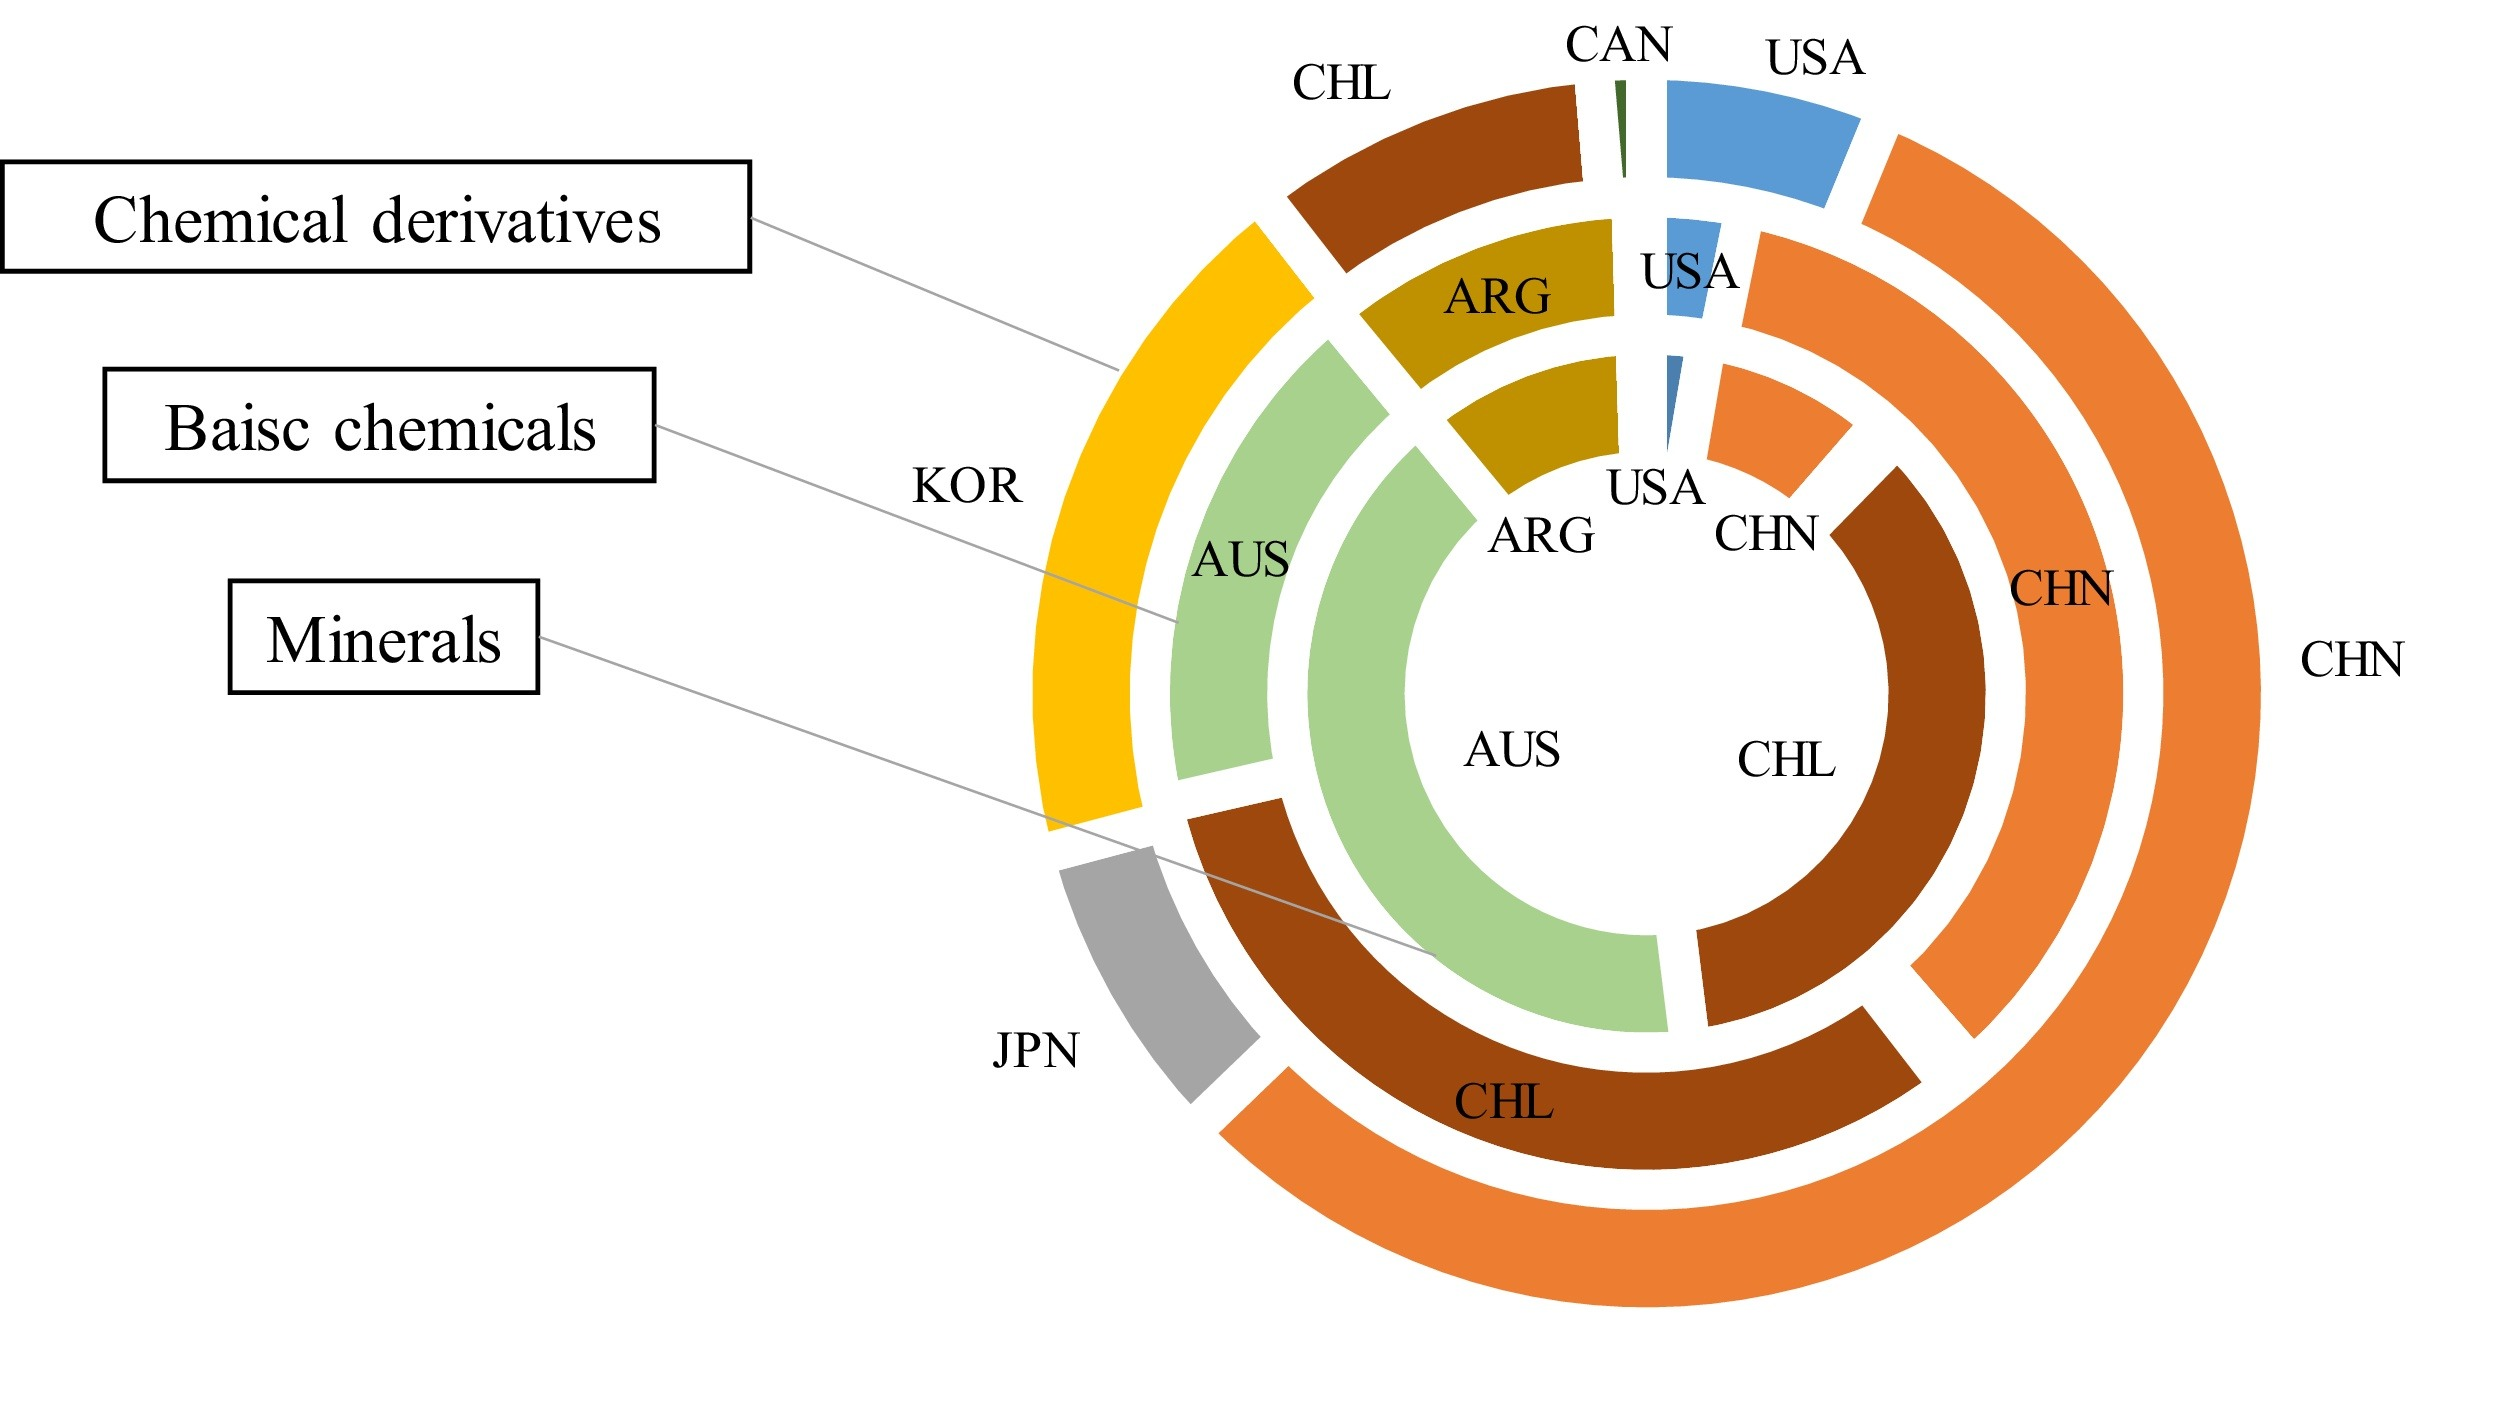
\includegraphics[width=\textwidth]{Images/supply_chain/1-s2.0-S0921344917301118-gr5_lrg.jpg}
    \caption{Répartition de l'extraction et du raffinage du lithium par pays}
    \label{fig:lithium_country}
\end{subfigure}
\hfill
\begin{subfigure}{0.4\textwidth}
    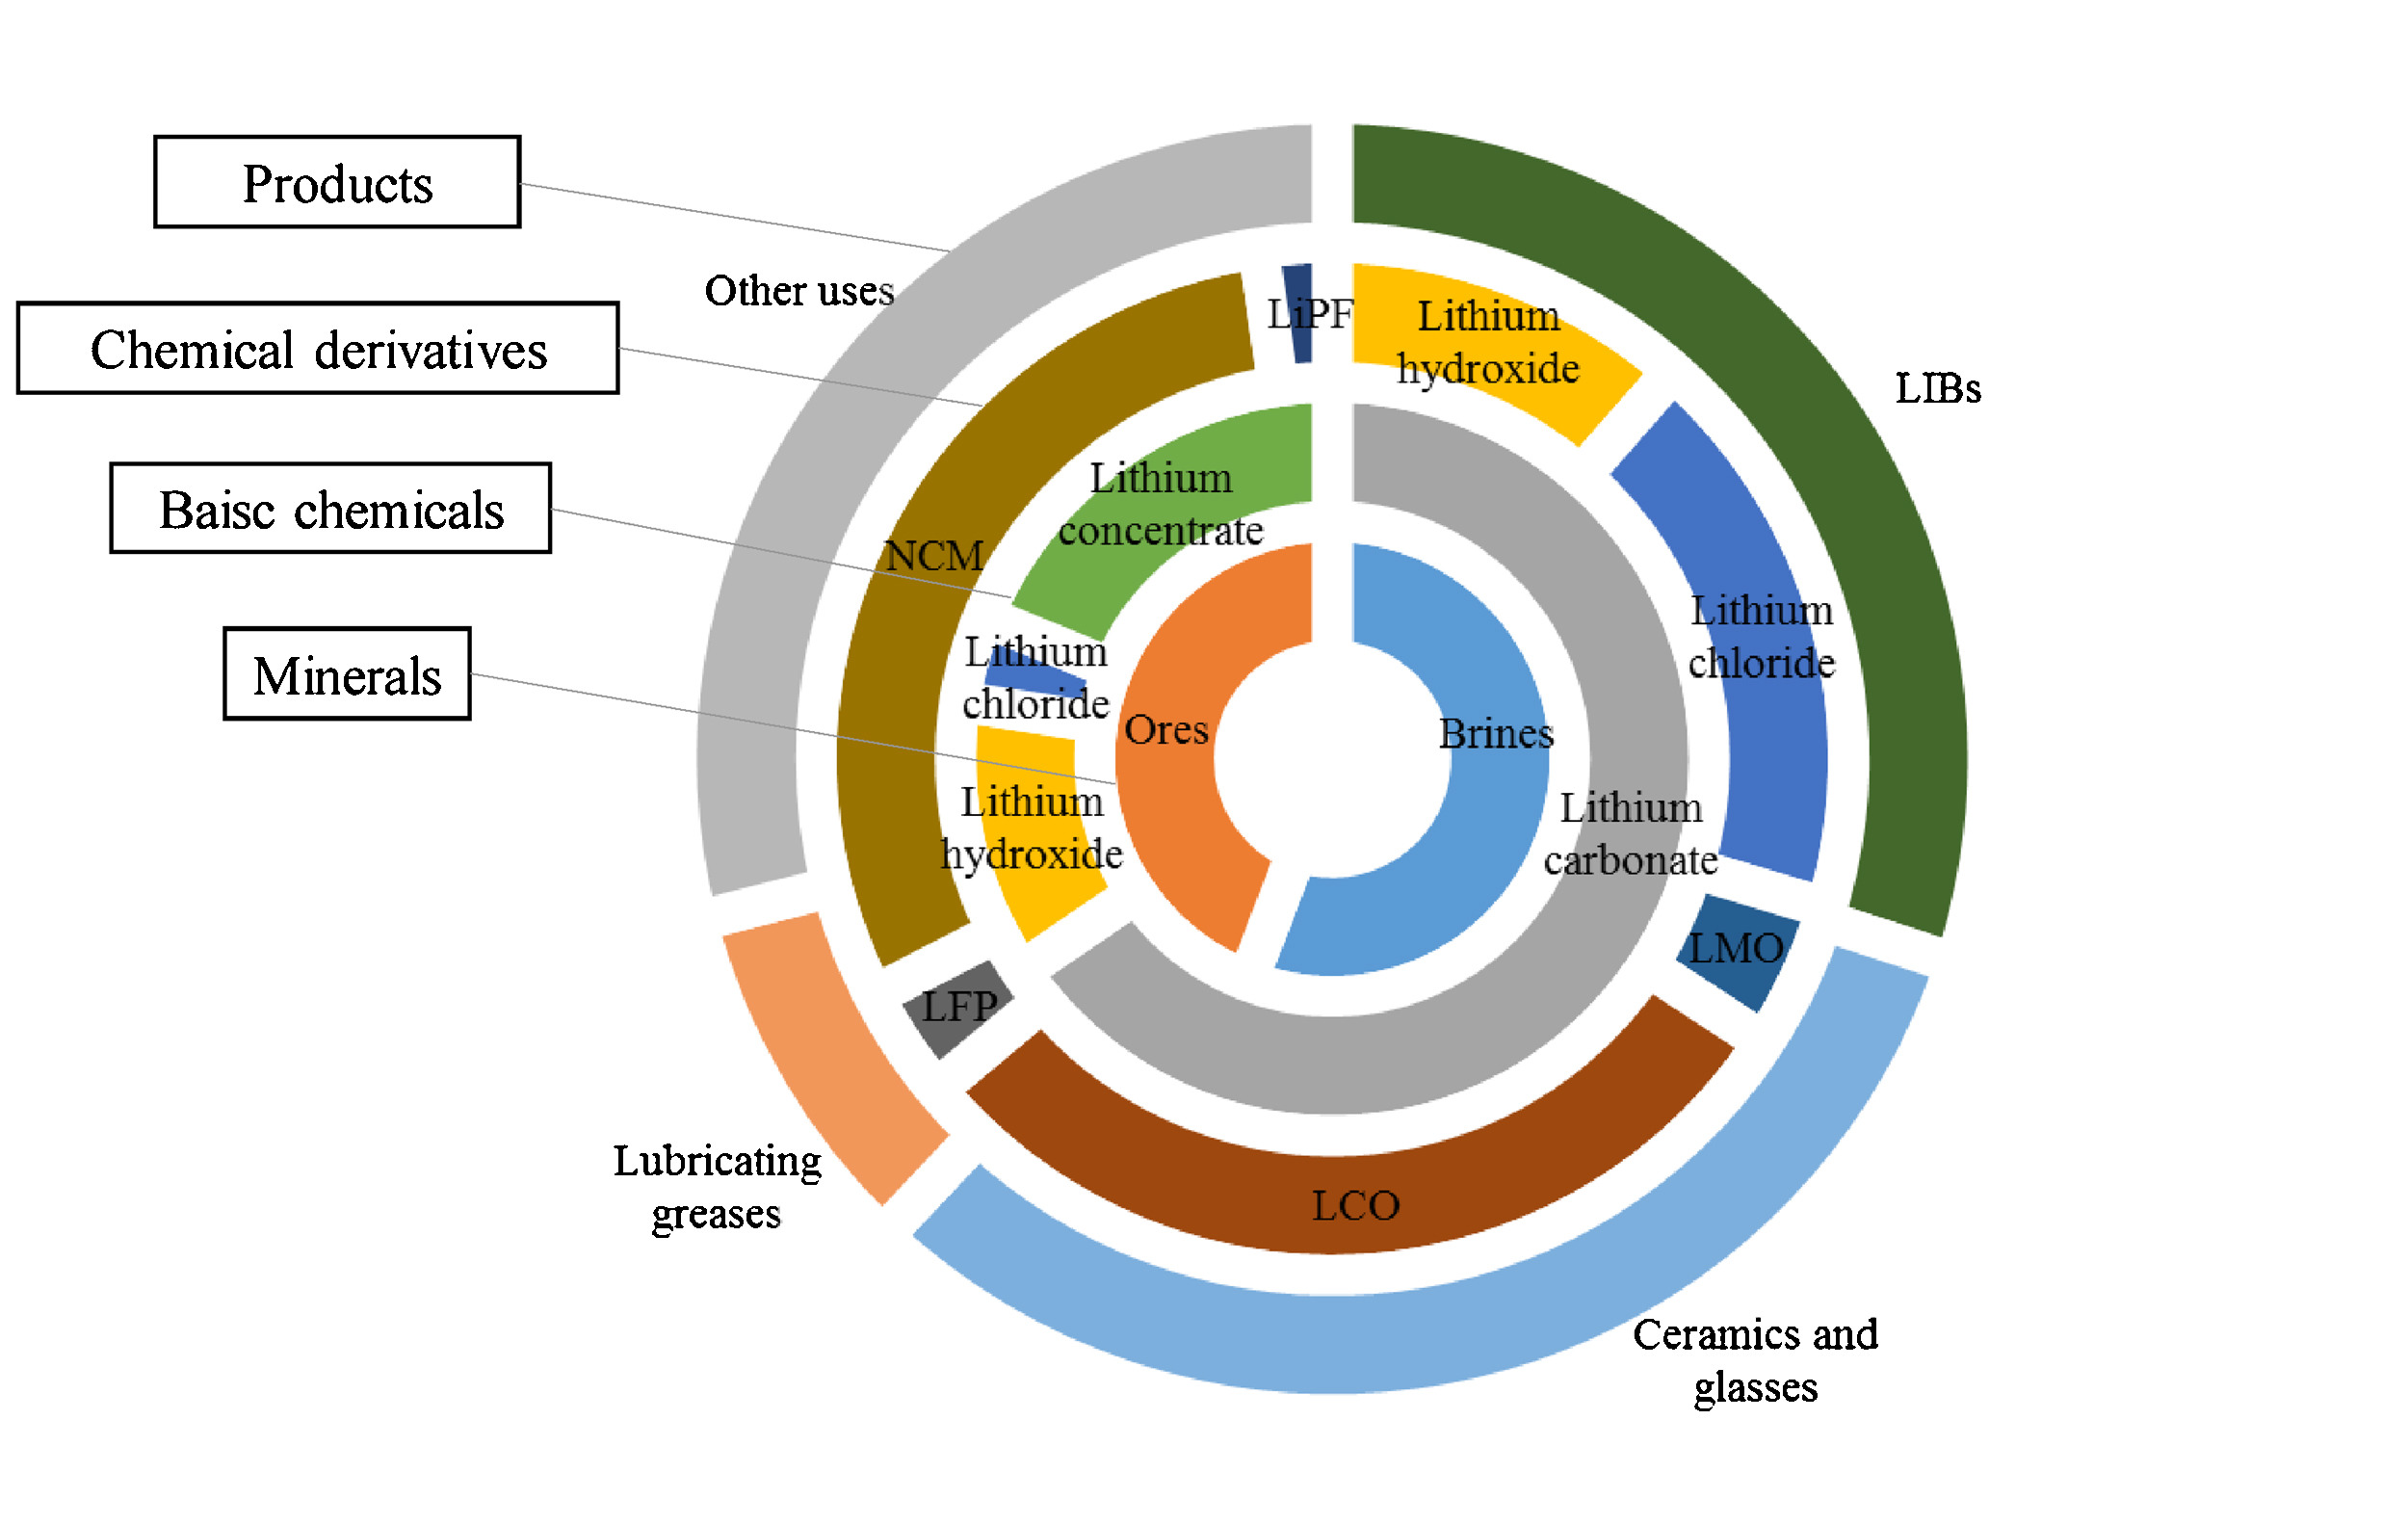
\includegraphics[width=\textwidth]{Images/supply_chain/1-s2.0-S0921344917301118-gr6_lrg.jpg}
    \caption{Répartition de la chaine de valeur du lithium par type de produits}
    \label{fig:lithium_type}
\end{subfigure}
\hfill
\begin{subfigure}{0.4\textwidth}
    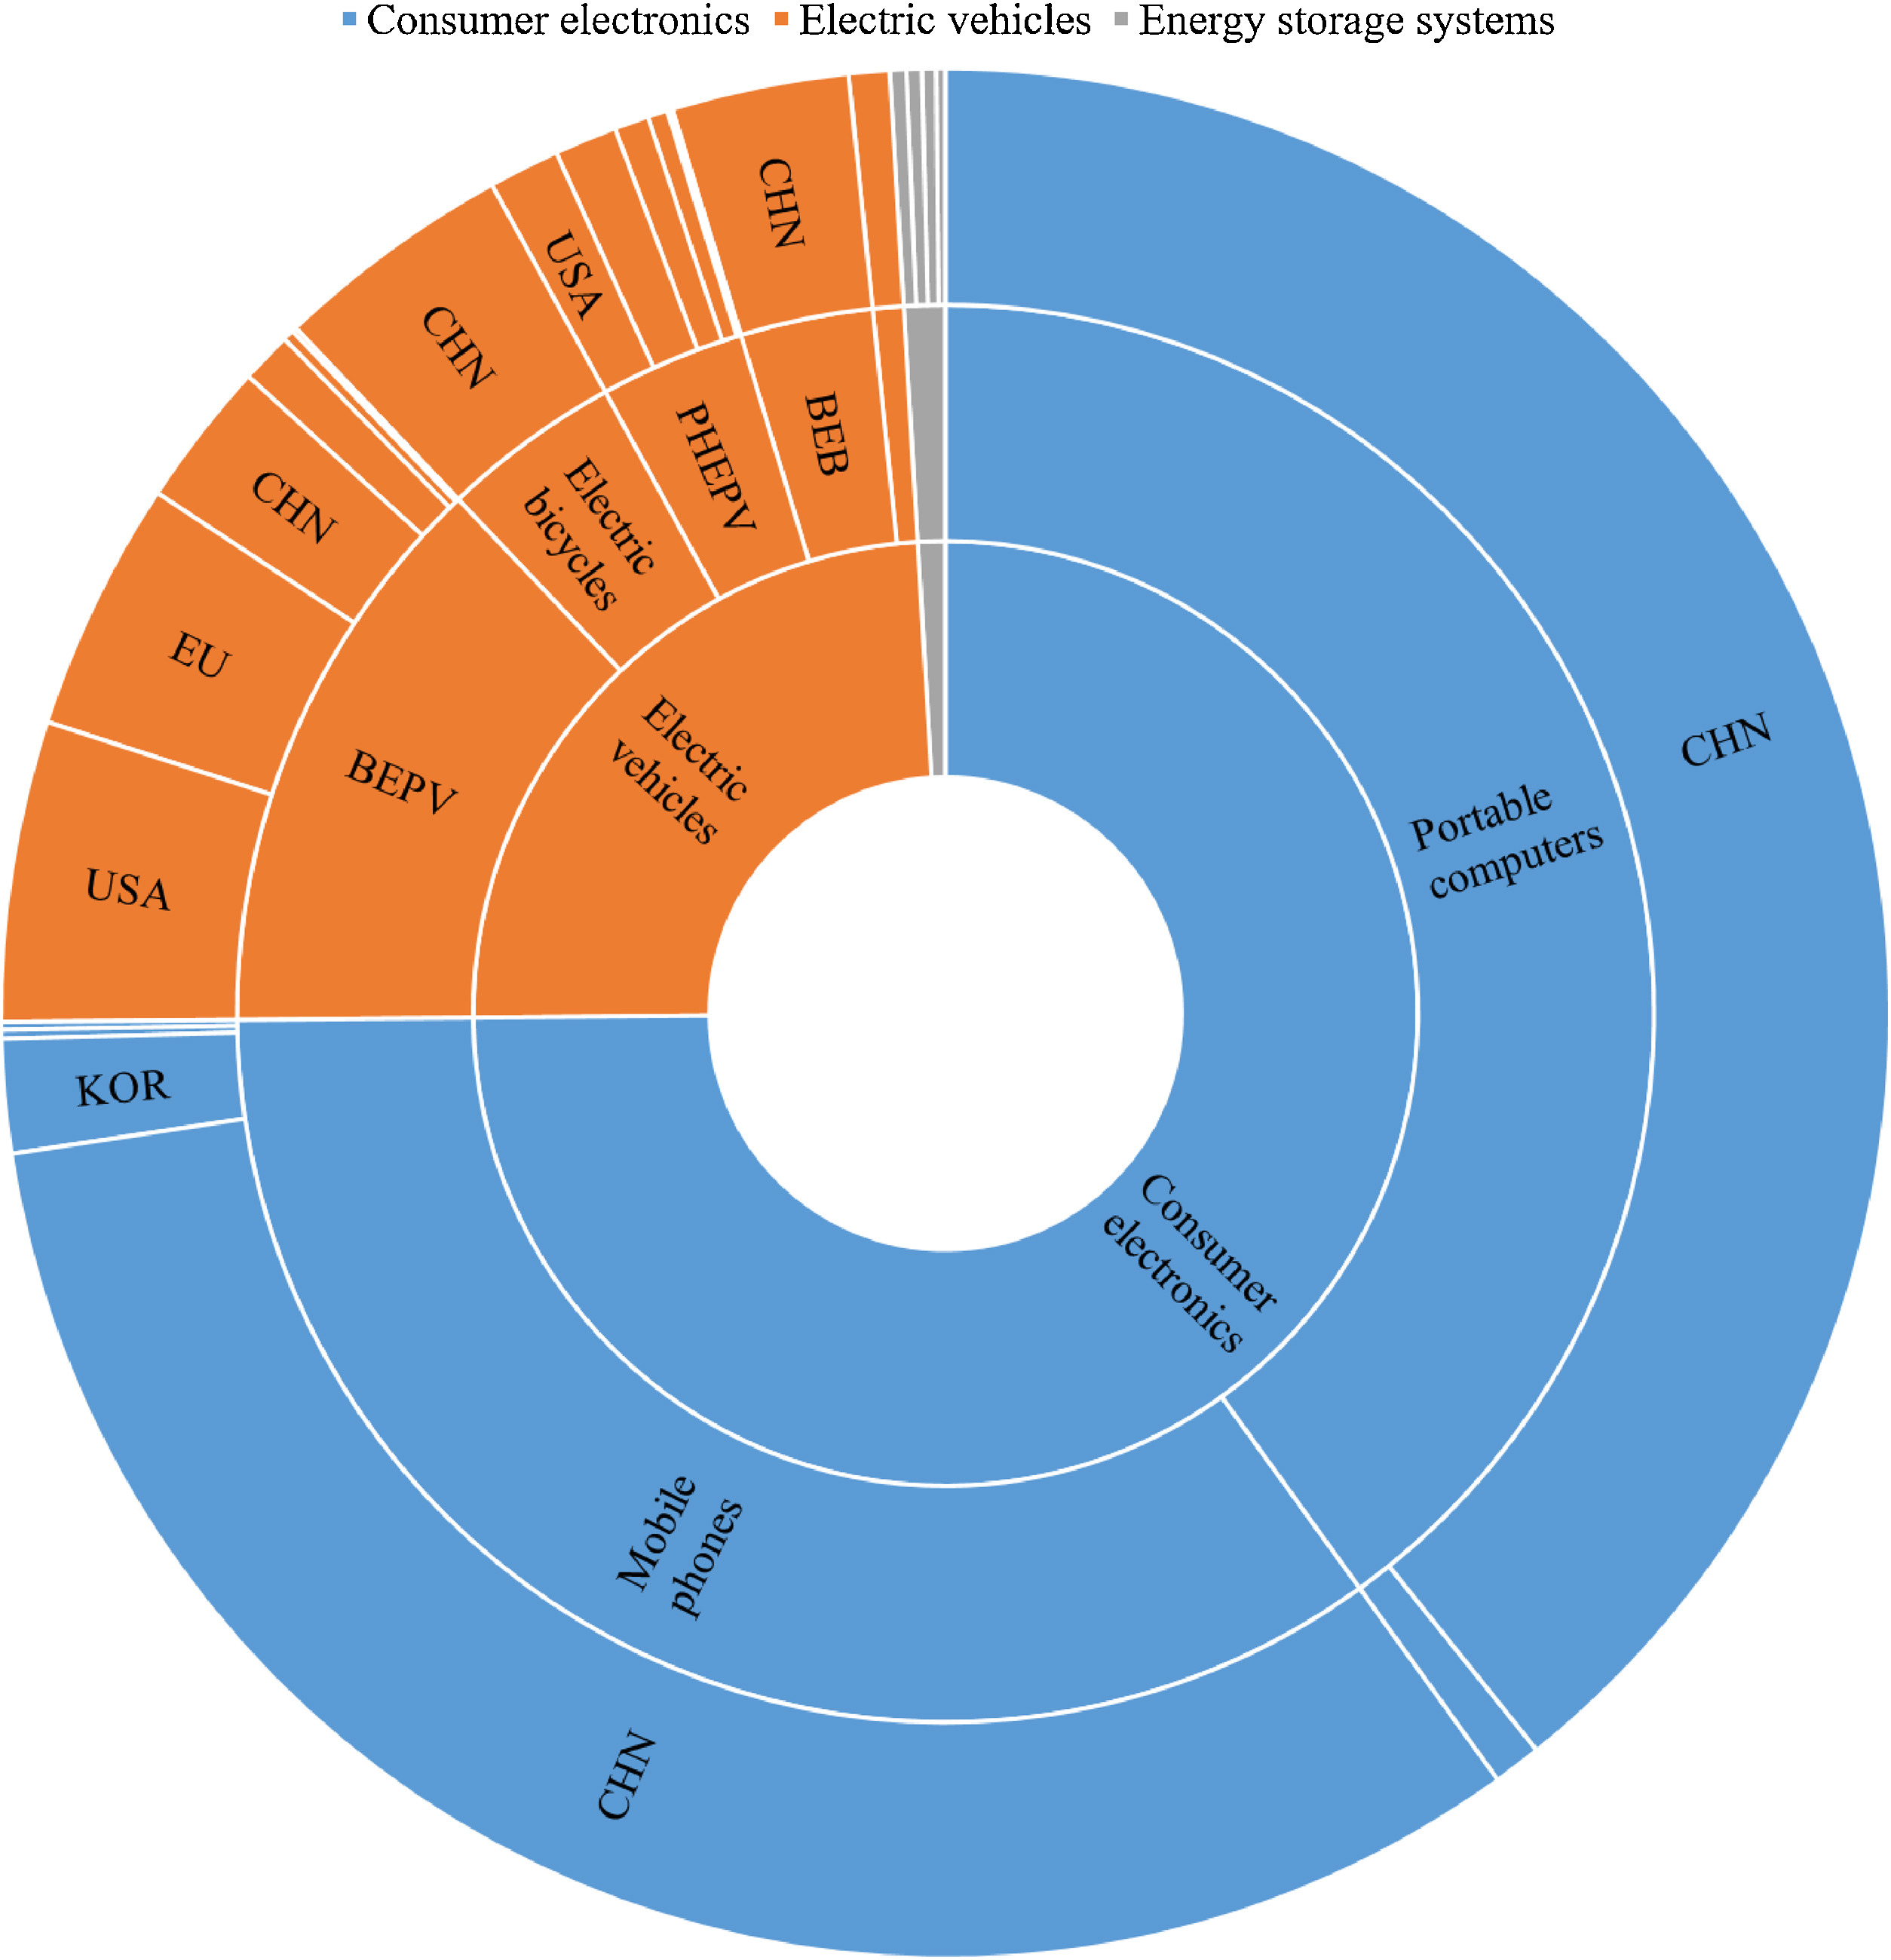
\includegraphics[width=\textwidth]{Images/supply_chain/1-s2.0-S0921344917301118-gr7_lrg.jpg}
    \caption{Répartition de la consommation de batterie lithium-ion (LIBs) par usage}
    \label{fig:LIB_use}
\end{subfigure}
        
\caption{Chaine d'approvisionnement issue du lithium (\cite{sun_tracing_2017})\\}
\caption*{Note : La chaine d'approvisionnement évolue très rapidement, les données présentées peuvent devenir obsolètes à moyen terme}
\label{fig:lithium_supply_chain}
\end{figure}

Les systèmes énergétiques décarbonés seront dépendants de chaînes d'approvisionnement plus complexes - illustré par la multiplicité des produits en figure \ref{fig:lithium_type}- avec une valeur ajoutée très importante à l'aval de l'extraction. Dans la continuité de la section précédente, cette section expose les enjeux géopolitiques autour de la maîtrise industrielle et technologique à l'aval de l'extraction.\smallbreak
Cette section présentera un état des lieux de l'industrie bas-carbone actuellement dominée par l'industrie chinoise. La figure \ref{fig:lithium_country} illustre l'importance de la Chine dans le raffinage du lithium, mais l'industrie chinoise a un poids bien plus important dans d'autres technologies bas-carbone.\smallbreak
Les enjeux géopolitiques dépendent de la capacité des industries à réagir à des évènements géopolitiques. Pour cette raison, cette section abordera les temporalités dans les chaînes d'approvisionnement. Les temps de déploiement de nouveaux site de production sur l'ensemble de la chaîne de valeur seront discutés : des temps très longs au niveau de l'extraction et relativement moyens pour les maillons de production proches de l'utilisation finale.\smallbreak
Enfin, cette section discutera de plusieurs leviers pour améliorer la sécurité et la résilience des approvisionnements. Elle abordera d'une part le rôle de la maîtrise technologique pour améliorer la substituabilité des métaux et d'autre part le rôle du recylage pour réduire les tensions d'approvisionnement.

    \newpage
    \subsection{Etat des lieux de l'industrie des technologies bas-carbone}
    \label{section:etat_des_lieux}
    L'utilisation de métaux par les technologies bas-carbone s'intensifie dans les scénarios ambitieux de décarbonation. Les principales technologies responsables de cette intensification sont les réseaux électriques d'une part et les véhicules électriques d'autre part. Comme exposé en figure \ref{fig:metals_demand} la consommation en cobalt pour la fabrication des batteries des véhicules électriques pourrait dépasser la consommation mondiale pour tout les usages de cobalt en 2021.\smallbreak
L'aval de ces matières brutes - illustré en figure \ref{fig:supply_key_elements} - est constitué de deux étapes capitales pour l'approvisionnement : le raffinage et la fabrication des composants intermédiaire.\smallbreak
L'étape de raffinage est actuellement dominée par l'industrie chinoise dans l'ensemble des métaux critiques pour la décarbonation (voir fiches métaux section \ref{section:approvisionnement}). De manière générale, chaque métal possède au moins un type de chaîne d'approvisionnement pour le raffinage. Mais les métaux peuvent avoir plusieurs filières de raffinage en raison de la diversité de leur état au moment d'extraction. Par exemple, le nickel issu de minerai d'oxyde est particulièrement difficile à convertir en nickel de classe 1 (très pur) contrairement à du nickel issu de minerai de sulfure (\cite{iea_role_2021}).\smallbreak
La Chine possède aussi une place très dominante dans la fabrication des composants, voire sur la fabrication finale de la technologie. L'étape de fabrication des composants peut se décomposer en plusieurs sous-étapes. La fabrication des batteries est précédée de celle de l'anode et de la cathode. Cette dernière concentre la majorité des enjeux d'approvisionnement (voir figure \ref{fig:EV_key_elements}). Les chaînes d'approvisionnement autour des installations photovoltaïques et éoliennes contiennent également plusieurs maillons comme présenté en figure \ref{fig:electricity_key_elements}.\smallbreak
Même si l'explosion de la demande en véhicules électriques et en installations photovoltaïques et éoliennes offre la possibilité à d'autres pays de saisir la croissance des marchés, les projets industriels en développement placent progressivement l'industrie chinoise dans une position encore plus prépondérante. L'industrie chinoise pourrait être en mesure de satisfaire la demande en modules photovoltaïques dans les scénarios les plus ambitieux de décarbonation jusqu'en 2030 (\cite{iea_energy_2023}).\smallbreak
Il convient de noter que certains maillons du déploiement de technologies bas-carbone sont moins soumis aux risques géopolitiques : l'étude et le développement, l'installation et l'exploitation d'infrastructures. Néanmoins, il n'est pas garanti que la valeur ajoutée de ces maillons soit essentiellement locale. (voir encadré \hyperref[VAENR]{\textit{Répartition de la VA sur le PV et l'éolien en France}})
\begin{figure}[!b]
    \centering
    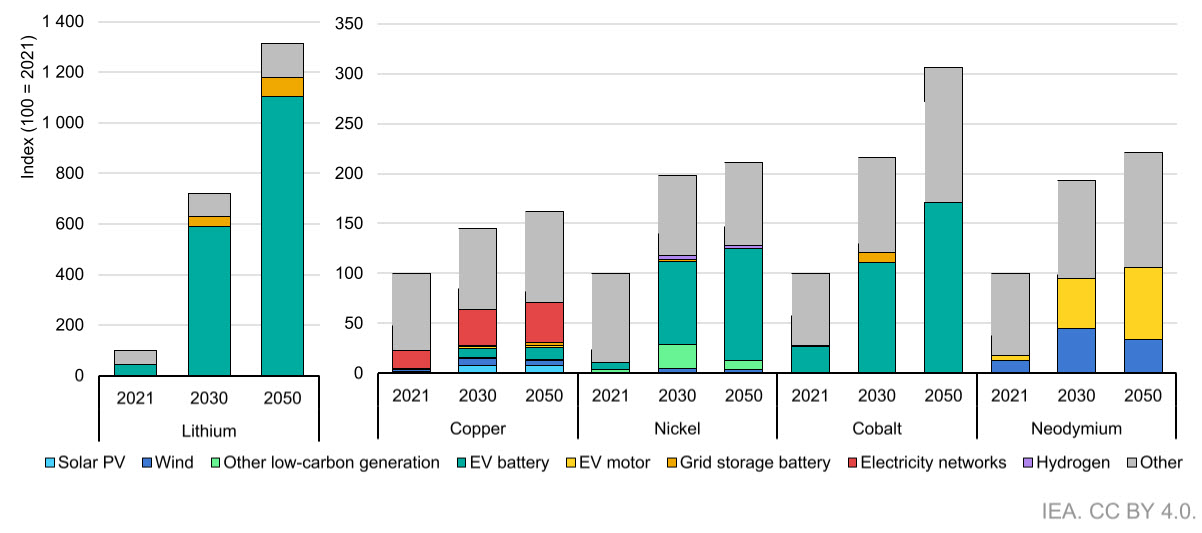
\includegraphics[width=\textwidth]{Images/supply_chain/metals_demand.jpg}
    \caption{Evolution de la demande en métaux dans lans le scénario NZE de l'AIE (\cite{iea_energy_2023})}
    \label{fig:metals_demand}
\end{figure}

\begin{figure}[!t]
\centering
\begin{subfigure}{0.9\textwidth}
    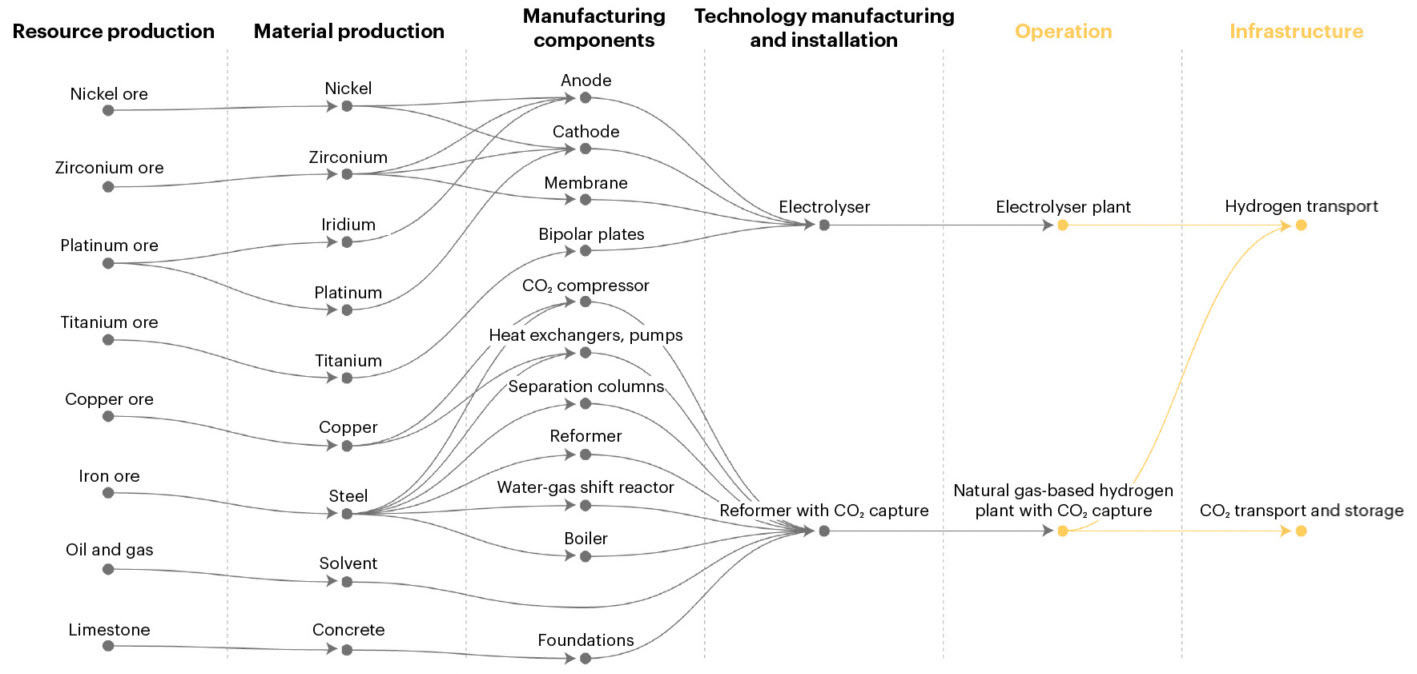
\includegraphics[width=\textwidth]{Images/supply_chain/key_elements_h2.jpg}
    \caption{Hydrogène bas-carbone}
    \label{fig:h2_key_elements}
\end{subfigure}
\hfill
\begin{subfigure}{0.9\textwidth}
    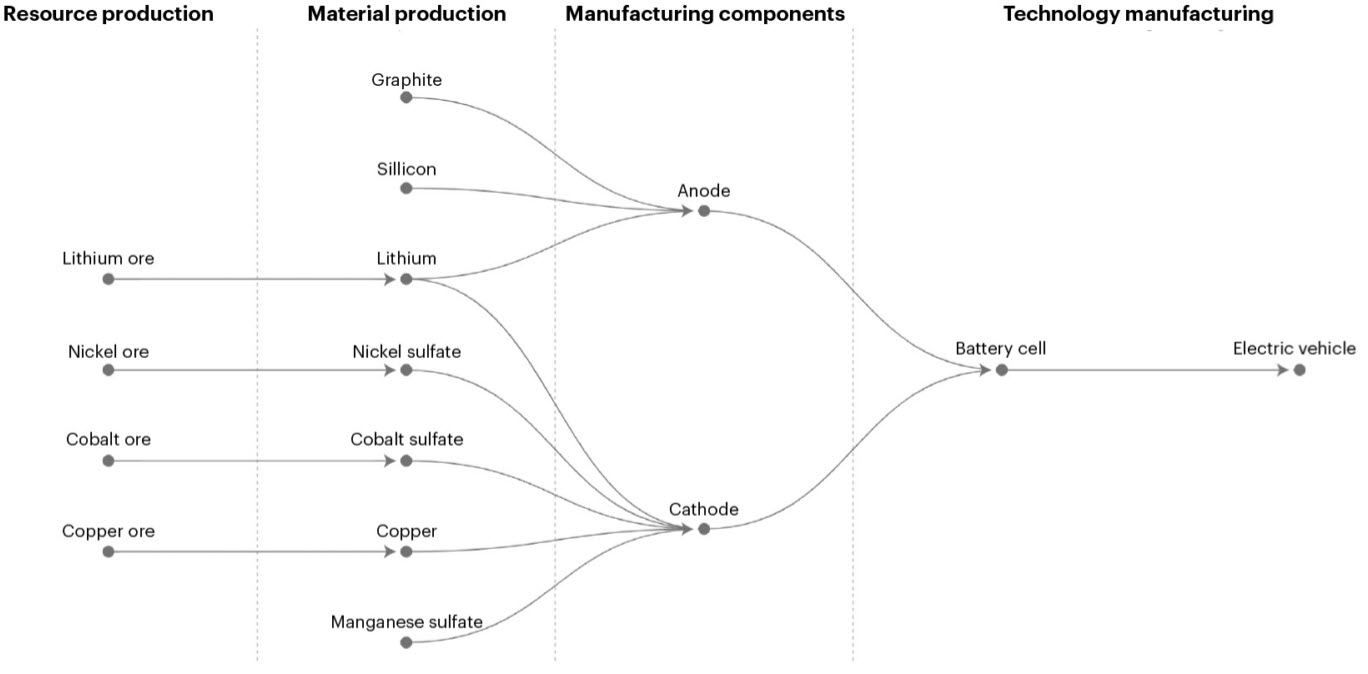
\includegraphics[width=\textwidth]{Images/supply_chain/key_elements_VE.jpg}
    \caption{Véhicules électriques}
    \label{fig:EV_key_elements}
\end{subfigure}
\hfill
\begin{subfigure}{0.9\textwidth}
    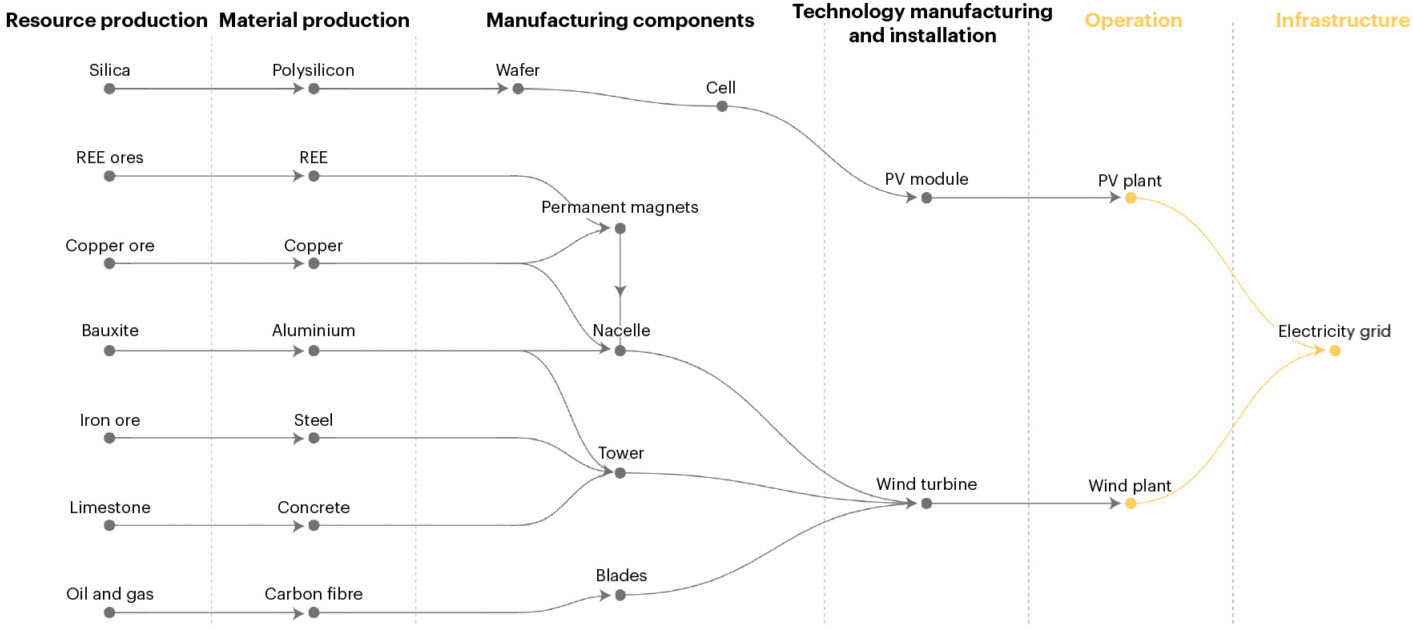
\includegraphics[width=\textwidth]{Images/supply_chain/key_elements_electricity.jpg}
    \caption{Electricité bas-carbone}
    \label{fig:electricity_key_elements}
\end{subfigure}  
\caption{Eléments clés des chaînes d'approvisonnements des technologies bas-carbone (\cite{iea_energy_2023})\\}
\label{fig:supply_key_elements}
\end{figure}
\clearpage
\begin{center}
    \boxput*(0,1){
        \colorbox{white}{Répartition de la valeur ajoutée sur le photovoltaïque et l'éolien en France}
    }{
    \setlength{\fboxsep}{15pt}
    \fbox{\begin{minipage}{14cm} 
    
    \begin{center}
        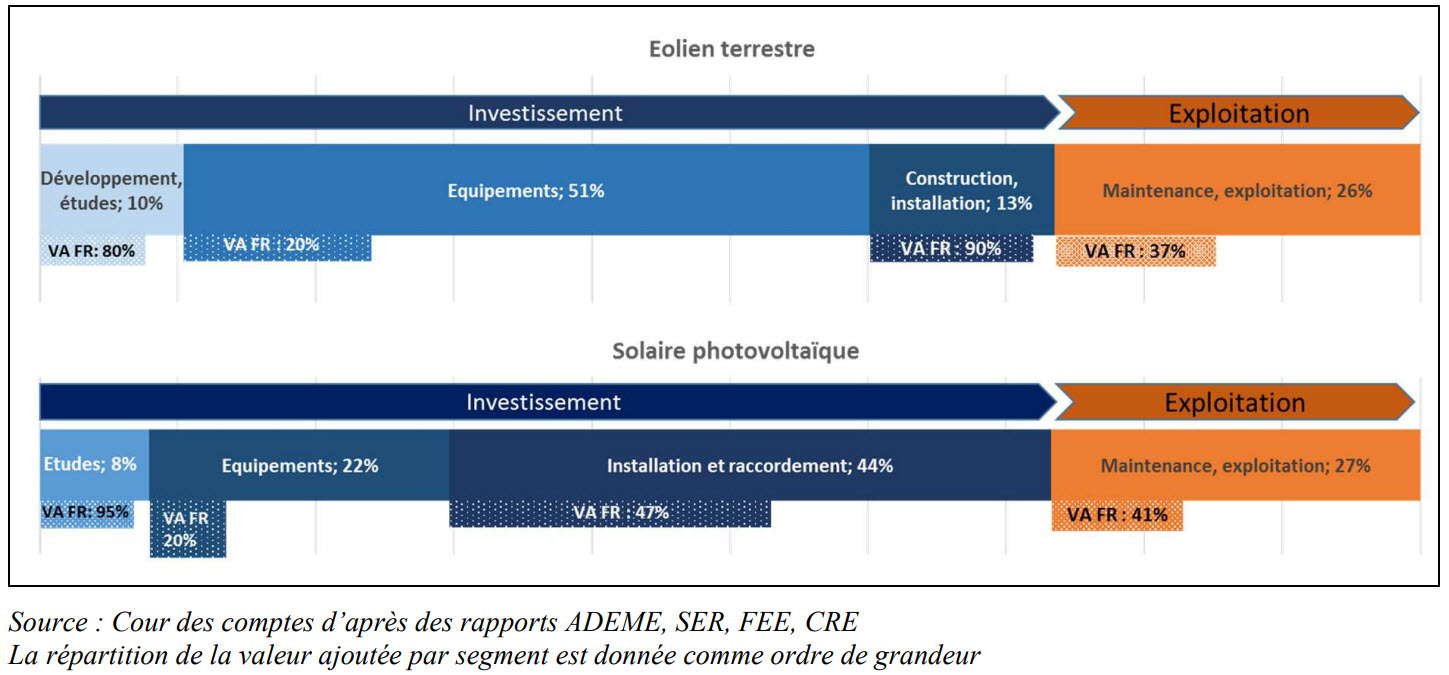
\includegraphics[width=\textwidth]{Images/supply_chain/VA_eolien_PV_cour.jpg}
\end{center}
    
Dans le domaine des énergies renouvelables, la chaîne de valeur comprend un grand nombre d'activités différentes. Ces activités incluent les études et l'ingénierie en amont, la fabrication de matériel et d'équipements, la construction et l'installation, l'exploitation et la maintenance, et enfin le démantèlement et le recyclage en aval.\smallbreak
Par exemple, dans le secteur du solaire, la France dispose de deux entreprises de fabrication intégrée de module photovoltaïque. Photowatt fait partie du groupe EDF et maîtrise l'ensemble de la fabrication des modules photovoltaïques, de la fabrication du lingot à partir de silicium jusqu'au recyclage (à 96\%). SunPower fait partie du Groupe TotalEnergies. La capacité de production reste néanmoins faible par rapport au marché français : environ 200 MWc par an pour Photowatt et moins de 100 MWc par an pour SunPower.\smallbreak
La France ne dispose pas d'ensemblier d'éolien terrestre et a perdu ses champions sur l'éolien en mer. Après s’être lancé en 2007 dans l’éolien en mer, Areva a cédé, en septembre 2016, ses activités à l’entreprise Gamesa, son partenaire espagnol dans la co-société Adwen. Le modèle de turbine Siemens sera fabriqué dans les deux futures usines construites au Havre. L’usine de fabrication d’éoliennes de Saint-Nazaire d’Alstom, a quant à elle été reprise par General Electric fin 2015.\smallbreak
De manière générale, il a été évalué qu'en France 40\% de la chaîne de valeur de l'éolien et du photovoltaïque est française. D'après le président directeur-général d'EDF, une chaîne de valeur 100\% française de l'éolien et du PV implique une hausse des coûts de l'ordre de 20\%.
\\[0.5cm]
\textit{Sources : \cite{cour_des_comptes_soutien_2018},\cite{photowatt_photowatt_2022},\cite{totalenergies_energie_2012},\cite{noauthor_souverainete_2023}}

    \end{minipage}}
    }
\end{center}
\label{VAENR}
~\\
\textbf{Photovoltaïque}
\smallbreak
La Chine est de loin le plus grand fournisseur de composants dans chaque étape de la chaîne d'approvisionnement du photovoltaïque avec une capacité de production de 340 GW/an (voir figure \ref{fig:PV_sankey}). Cela est dû à des coûts de production très faibles en Chine (voir figure \ref{fig:PV_cost}). L'écart des coûts de production entre l'Europe et la Chine se joue sur plusieurs facteurs : le coût de l'énergie, le coût de la main d'oeuvre et le coût de la dépréciation. Si ce dernier est plus faible en Chine, c'est en grande partie dû au coût du capital plus faible dans ce secteur et à la grande taille des unités de production.\smallbreak
Bien qu'ayant permis une importante chute des prix du photovoltaïque, la domination chinoise place les pays européens ambitieux quant au développement de cette technologie dans une situation de dépendance. Une sortie de cette dernière imposerait aux pays européens un coût d'investissement d'environ 500 M€ par GW de production photovoltaïque intégré (voir figure \ref{fig:PV_investment}).

\begin{figure}[!t]
\centering
\begin{subfigure}{0.8\textwidth}
    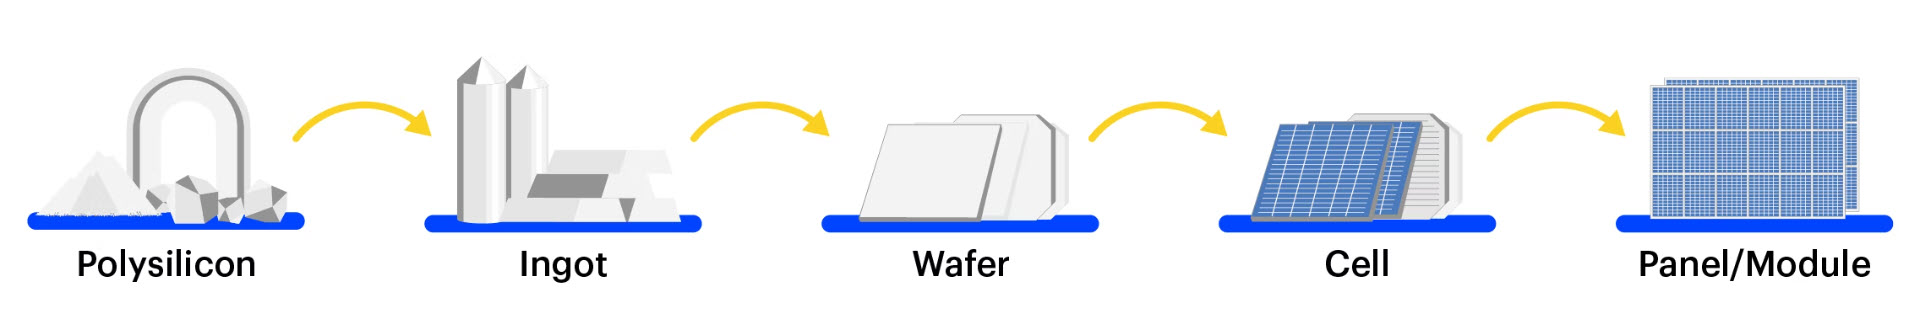
\includegraphics[width=\textwidth]{Images/supply_chain/PV_supply_chain.jpg}
    \caption{Etapes de fabrication d'un module photovoltaïque}
    \label{fig:PV_supply}
\end{subfigure}
\hfill
\begin{subfigure}{0.8\textwidth}
    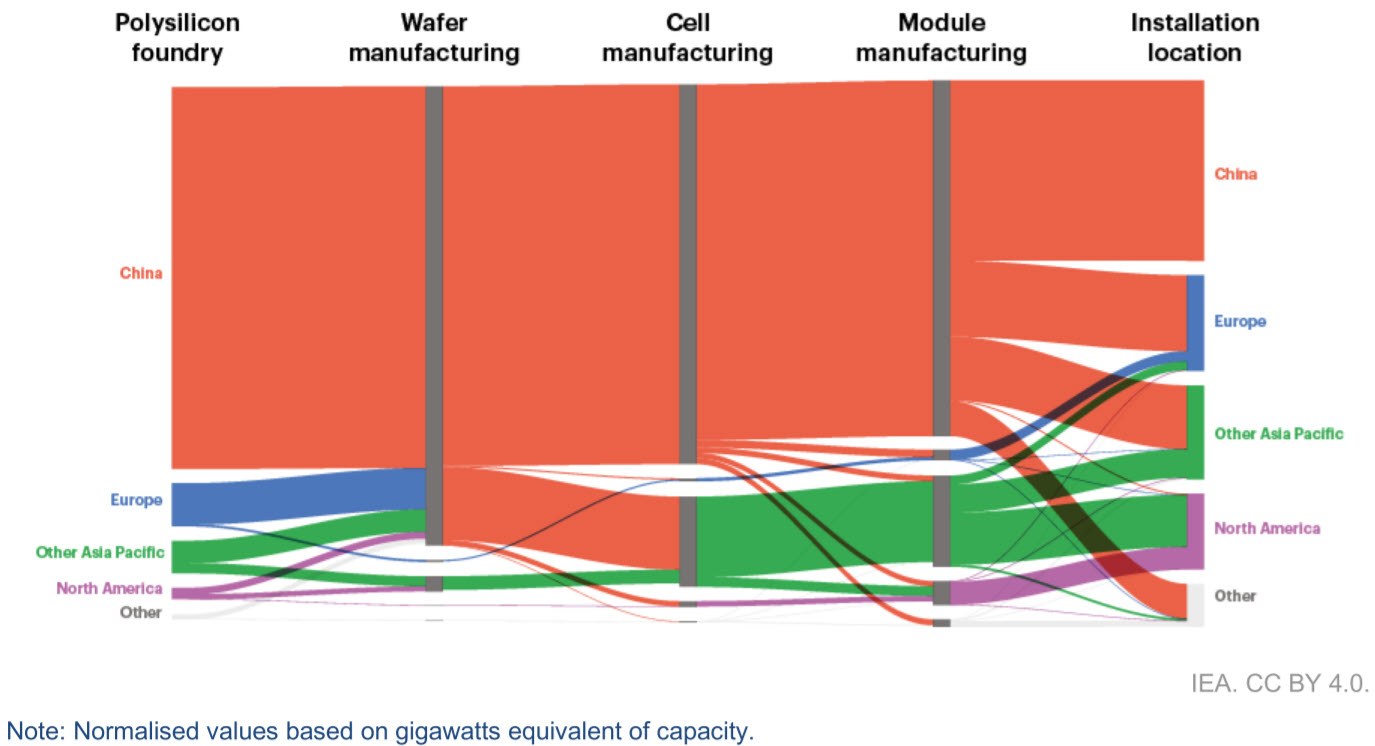
\includegraphics[width=\textwidth]{Images/supply_chain/sankey_diagram_PV_bis.jpg}
    \caption{Flux mondiaux de la chaîne d'approvisionnement du photovoltaïque \cite{iea_energy_2023}}
    \label{fig:PV_sankey}
\end{subfigure}
\hfill
\begin{subfigure}{0.8\textwidth}
    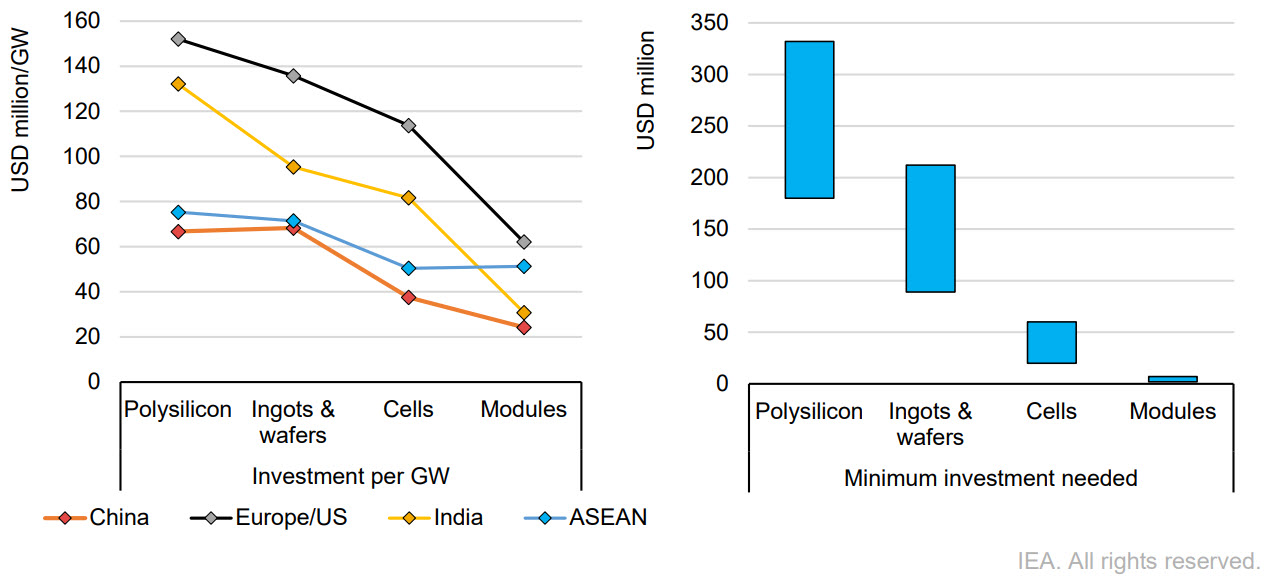
\includegraphics[width=\textwidth]{Images/supply_chain/PV_investment.jpg}
    \caption{Coût d'investissement (gauche) et investissements minimum requis (droite) par étape de la chaîne d'approvisionnement \cite{iea_special_2022}}
    \label{fig:PV_investment}
\end{subfigure}
\begin{subfigure}{0.7\textwidth}
    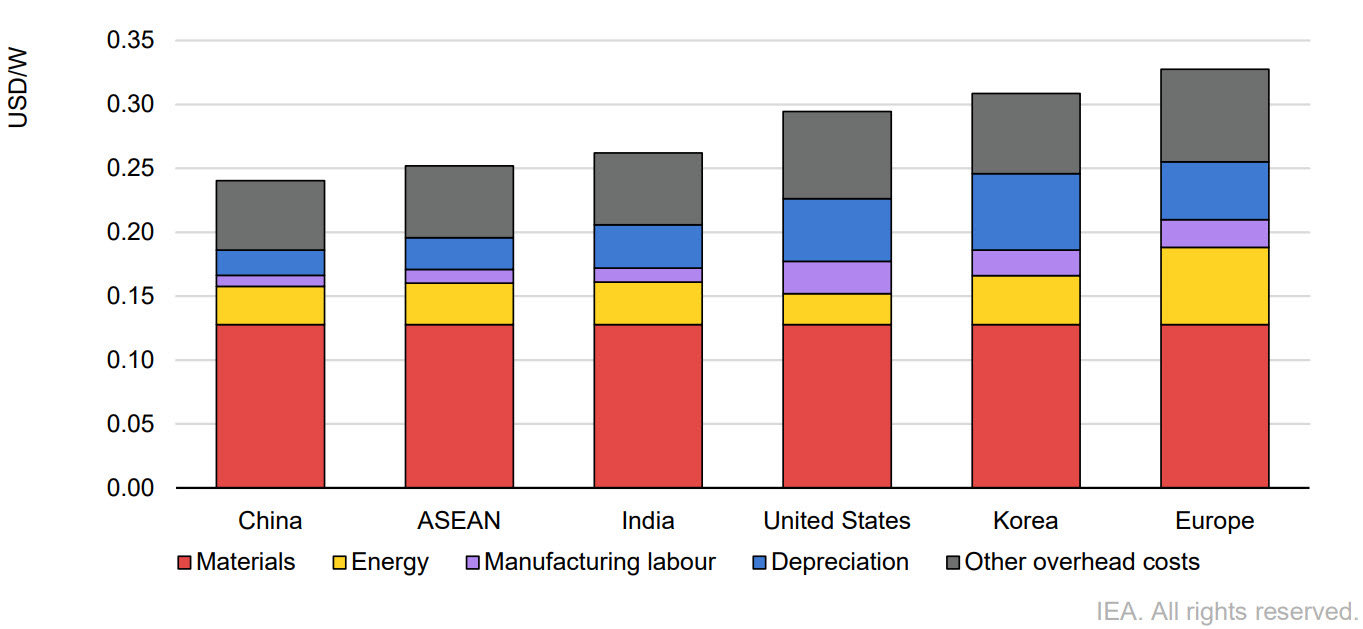
\includegraphics[width=\textwidth]{Images/supply_chain/PV_production_costs.jpg}
    \caption{Coût de production des composants photovoltaïque \cite{iea_special_2022}}
    \label{fig:PV_cost}
\end{subfigure}
  
\caption{Chaîne d'approvisionnement du photovoltaïque}
\label{fig:supply_key_elements_PV}
\end{figure}
\clearpage
\textbf{Eolien}
\smallbreak
Les composants d'une éolienne sont volumineux et lourds, ce qui pénalise une délocalisation de la production. Néanmoins, il est tout à fait possible d'avoir des marchés approvisionnés par une production étrangère. Le marché domestique des Etats-Unis est approvisionné à 75\% par des pales d'éoliennes étrangères (\cite{iea_energy_2023}). La Chine occupe une place importante dans les chaînes d'approvisionnement et représente plus de la moitié des exports de composants éolien (voir figure \ref{fig:wind_sankey}, volume d'exportation en US\$).
\smallbreak
La dépendance envers la Chine dans la filière éolienne est assez modérée. Cependant, il est possible que la Chine produise les composants d'éolienne à des coûts encore plus compétitifs. Le transport de ces éléments étant économiquement viable, il est possible que l'industrie chinoise s'impose sur l'ensemble des marchés mondiaux. Cela aurait pour conséquence de mettre ces marchés dans une situation équivalente aux marchés du photovoltaïque en matière de dépendance envers la Chine.
\begin{figure}[!h]
    \centering
    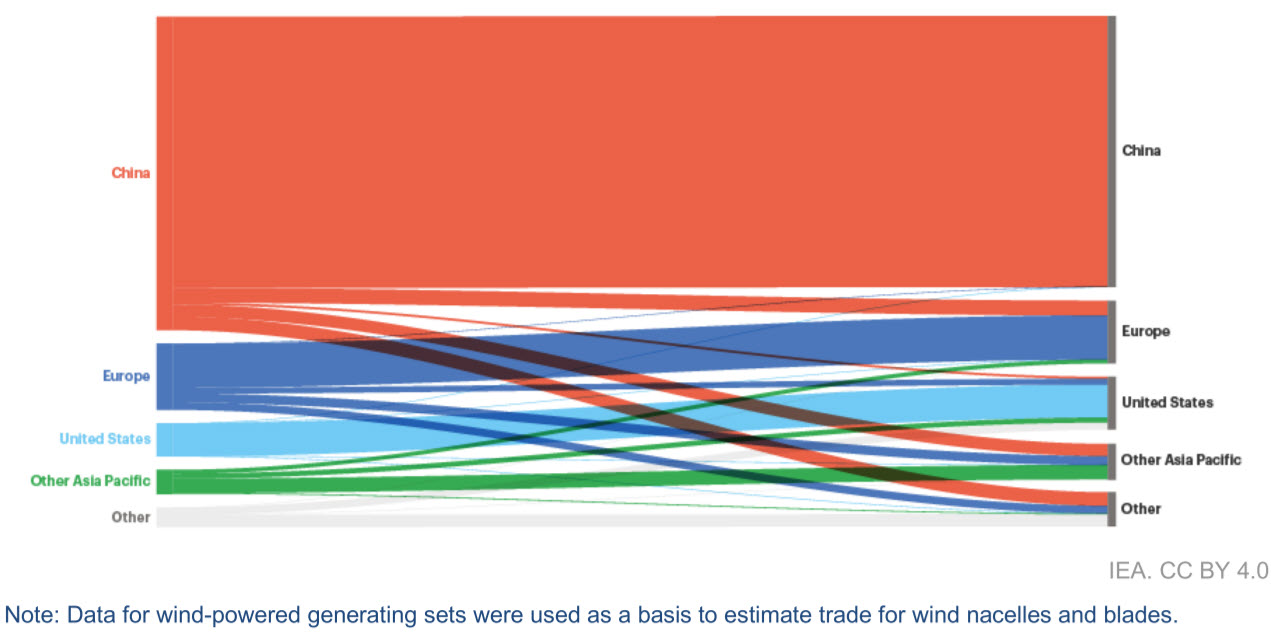
\includegraphics[width=0.8\textwidth]{Images/supply_chain/sankey_diagram_wind.jpg}
    \caption{Flux d'échanges de composants d'éolien (nacelles et pales) en US\$ (\cite{iea_energy_2023})}
    \label{fig:wind_sankey}
\end{figure}
~\\
\textbf{Véhicules électriques}
\smallbreak
Le marché des véhicules électriques est en pleine explosion en partie grâce aux politiques publiques. La Chine occupe une double place dans le marché mondial des véhicules électriques. L'industrie chinoise est la première industrie productrice et exportatrice de batteries pour véhicules électriques et de véhicules électriques (voir figure \ref{fig:EV_sankey}). Le marché chinois du véhicules électriques est quant à lui le plus important dans le monde (en terme de nombre de véhicules vendus).\smallbreak
La production américaine de véhicules électriques repose nettement moins sur les batteries chinoises que la production européenne. Cet écart s'explique en grande partie par des actions publiques américaines pour favoriser les batteries produites localement dès 2009, tandis que l'Union européenne a mis en place une stratégie industrielle sur les batteries en 2017.\smallbreak
L'industrie automobile est souvent un secteur très important de l'économie des pays européens. La décarbonation conduit cette industrie exclusivement vers la production de véhicules électriques dépendants d'un approvisionnement en batterie. Cet approvisionnement en batterie vient actuellement à 15\% de Chine et cette part pourrait augmenter si les capacités de production européennes de batteries n'augmentent pas aussi vite que le marché. Cette situation permet à la Chine d'affecter directement un secteur industriel très important pour l'économie européenne.\smallbreak
Grâce à des coûts de production faibles et à un marché important, la Chine attire les constructeurs de véhicules électriques étrangers. La majeure partie des véhicules électriques importés de Chine sont de constructeurs européens ou américains (voir figure \ref{fig:EV_Europe}).
\begin{figure}[!h]
\centering
\begin{subfigure}{0.8\textwidth}
    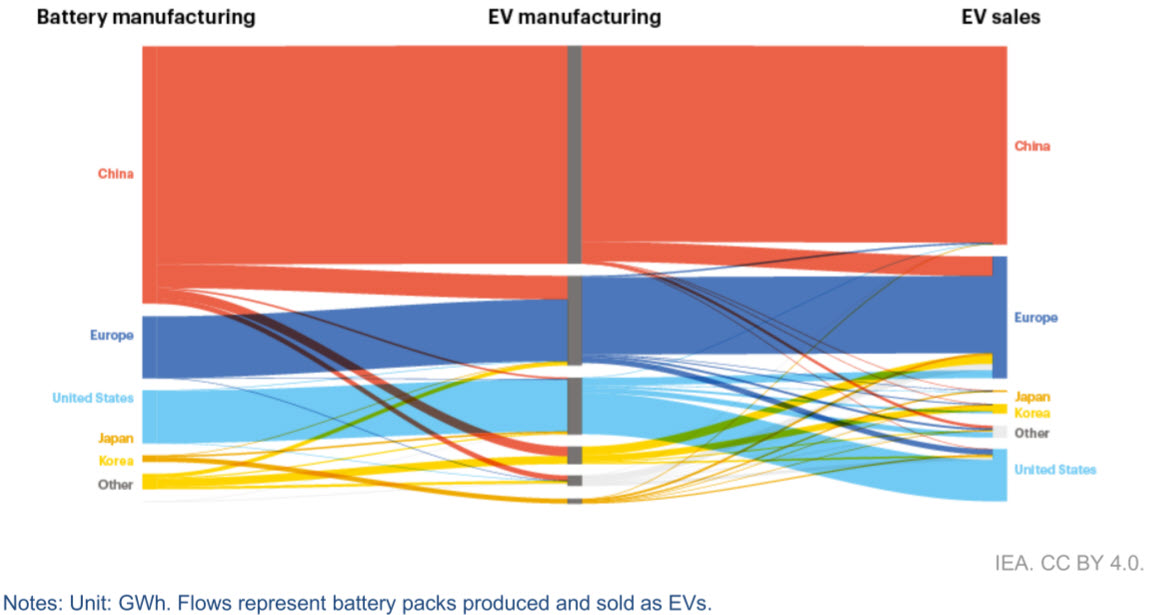
\includegraphics[width=\textwidth]{Images/supply_chain/sankey_diagram_EV.jpg}
    \caption{Flux mondiaux de la chaîne d'approvisionnement des véhicules électriques}
    \label{fig:EV_sankey}
\end{subfigure}
\hfill
\begin{subfigure}{0.8\textwidth}
    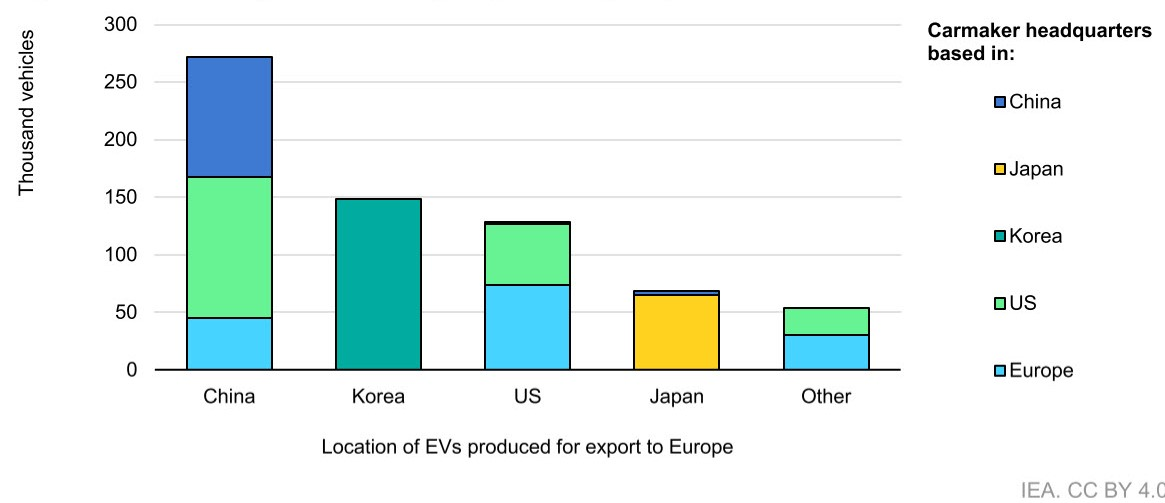
\includegraphics[width=\textwidth]{Images/supply_chain/Europe_EV_imports_bis.jpg}
    \caption{Répartition des importations de véhicules électriques en Europe par pays et par nationalité de fabricant}
    \label{fig:EV_Europe}
\end{subfigure}

\caption{Chaîne d'approvisionnement des véhicules électriques (\cite{iea_energy_2023})}
\label{fig:supply_key_elements_EV}
\end{figure}
\clearpage
    \subsection{Temporalités des chaînes d'approvisionnement}
    \label{section:temporalité}
    \input{03 - Maitrise technologique et industrielle/02_Temporalités des chaines d'approvisionnement.tex}
    \subsection{Leviers de sécurisation et résilience}
    \label{section:levier}
    \input{03 - Maitrise technologique et industrielle/03_Leviers de résilience.tex}
    \clearpage
    \clearpage
    \printbibliography
    \clearpage
\end{refsection}
% 4
\newpage
\begin{refsection}
\section{Politiques publiques sur les chaînes d'approvisionnement}
\label{section:politiques_publiques}
\begin{figure}[!b]
    \centering
    \begin{subfigure}[b]{0.48\textwidth}
        \centering
         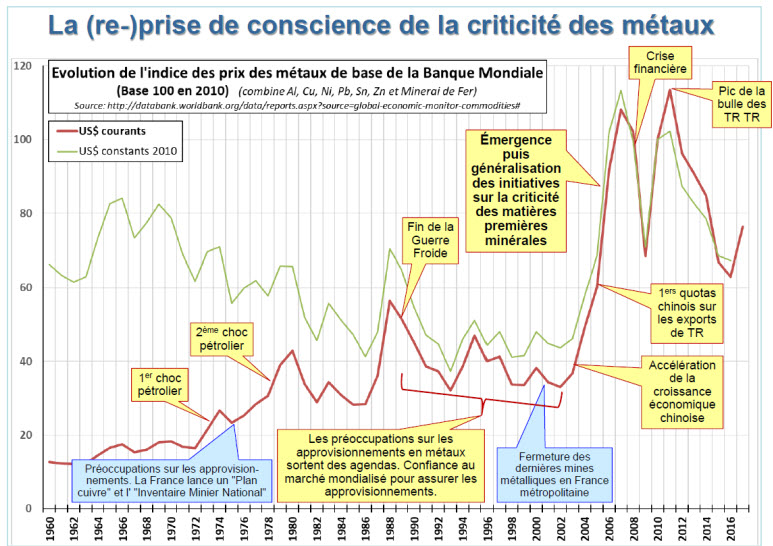
\includegraphics[width=\textwidth]{Images/Metals_policies/indice_metal.jpg}
         \caption{Indice des prix des métaux (\cite{brgm_substances_2022})}
         \label{fig:indices_metal}
    \end{subfigure}
    \hfill
    \begin{subfigure}[b]{0.48\textwidth}
        \centering
         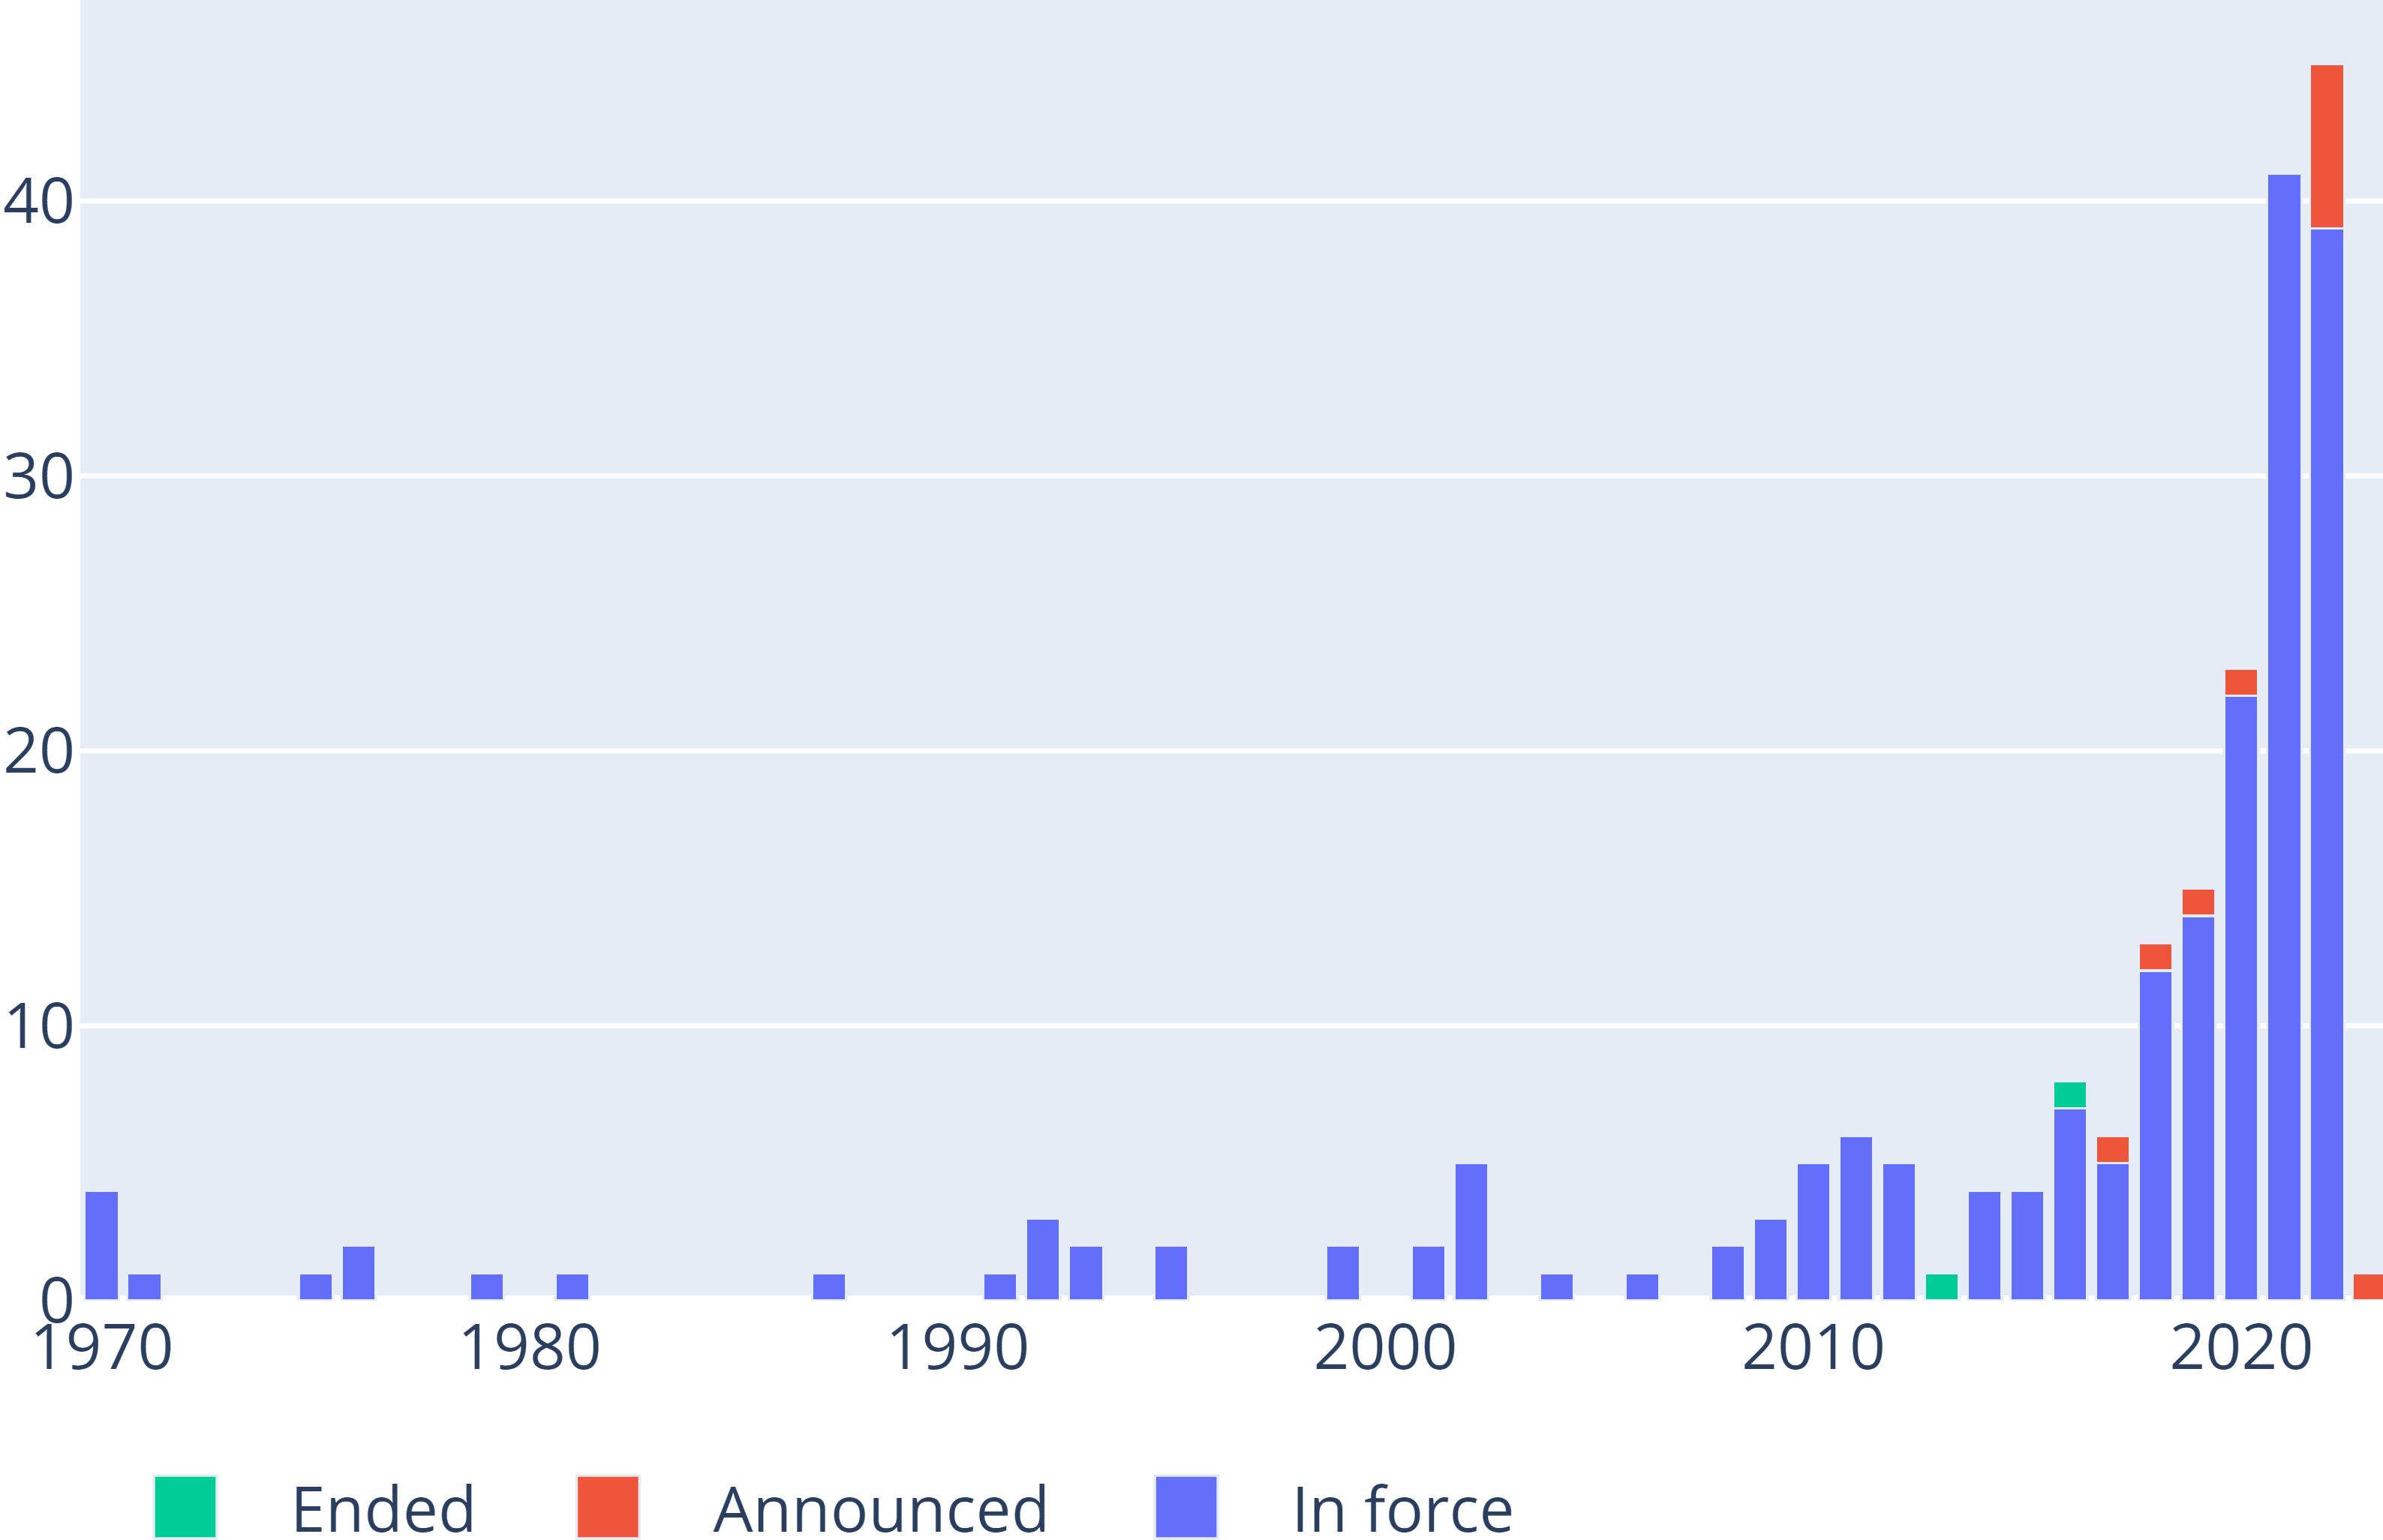
\includegraphics[width=\textwidth]{Images/Metals_policies/critical_metals_policies.png}
         \caption{Politiques publiques sur les métaux critiques (\cite{iea_critical_2022})}
         \label{fig:politiques_metal}
    \end{subfigure}
    \caption{Tendances historiques sur les métaux}
    \label{fig:metal_histoire}
\end{figure}
Les sections précédentes ont permis d'exposer certains risques géopolitiques pouvant être exacerbés par la décarbonation des mix énergétiques. Pour compléter cette étude, cette section propose une revue des politiques publiques sur les matériaux critiques dans le monde. L'objectif est d'apporter des éléments sur le caractère maîtrisable de ces risques géopolitiques.\smallbreak
L'approvisionnement en métaux est historiquement un enjeu militaire. La Guerre froide a engendré une course à l'armement et à l'espace, les industries militaires avaient alors le quasi-monopole de l'usages des métaux rares (\cite{donnen_vers_2022}). En 1950, le Congrès américain a adopté le \textit{'Defense Production Act'} pour conférer au président les pouvoirs nécessaires afin d'assurer l'approvisionnement en matériaux et les services nécessaires à la défense nationale, renonçant parfois aux exigences du commerce international. Initialement adoptée pour assurer la disponibilité du matériel de défense militaire pendant la guerre de Corée, le président Biden l'a invoquée pour sécuriser la production de vaccins COVID-19 en janvier 2021 et la production de lances à incendie en septembre 2021, afin d'atténuer les effets des incendies de forêt dans tout le pays (\cite{iea_critical_2022}).\smallbreak
La fin de la guerre froide a engendré une forte baisse des tensions sur l'approvisionnement avec d'une part la baisse de la demande des industries militaires et d'autre part la hausse de l'offre de la part des pays du bloc de l'Est. Cette relaxation a eu pour conséquence une diminution des prix des métaux (figure \ref{fig:indices_metal}) et une diminution des politiques publiques pour la sécurisation des approvisionnements en métaux. En France, la Caisse française des matières premières (CFMP) est dissoute en 1997. Elle assurait depuis 1980 la constition d'un stock stratégique de matières premières (\cite{donnen_vers_2022}).\smallbreak
A partir des années 2000, la croissance économique chinoise et la digitalisation de l'économie rendirent les chaînes d'approvisionnement à nouveau critiques. Cette tendance est amenée à s'amplifier avec les objectifs de décarbonation des pays du monde. La prise de conscience est visible à travers le nombre de politiques publiques sur les métaux critiques ces dernières années (figure \ref{fig:politiques_metal})\smallbreak
Cette section analyse les politiques publiques sur les chaînes d'approvisionnement en quatre parties. La première partie porte sur l'identification des faiblesses d'approvisionnement et leur importance par les politiques publiques. Les chaînes d'approvisonnement et les technologies bas-carbone étant complexes, l'identification et la quantification des risques est difficile. La deuxième partie porte sur les politiques publiques pour l'amélioration de la fiabilité des approvisionnements. La criticité des chaînes d'approvisionnement étant posée en première partie, la seconde partie développe les moyens de faire face à ces faiblesses. La troisième partie porte sur la maîtrise des chaînes de valeur. Cette partie se concentre plus sur la partie aval des deux parties précédentes, en abordant l'innovation et le recyclage. Enfin, la quatrième partie porte la durabilité de l'approvisionnement. En cohérence avec la décarbonation, une chaîne d'approvisionnement durable est bas-carbone. Le respect de normes environnementales et sociales des chaînes d'approvisionnement en augmenteront la fiabilité sur le long terme. 


\subsection{Analyse de risque}
\label{section:analyse_risque}
La première approche pour maîtriser les risques géopolitiques concernant la décarbonation est de disposer de moyens pour les identifier et les quantifier. Trois grandes familles de politiques publiques pouvant contribuer à analyser le risque géopolitique ont été analysées grâce à la base de données de l'AIE (\cite{iea_critical_2022}). Ces données permettent d'établir le tableau ci-dessous. Ce tableau permet de quantifier la distribution des politiques publiques dans le monde.
\begin{table}[!h]
\centering
\begin{tabular}{ |p{3cm}||p{3.5cm}|p{3.5cm}|p{3.5cm}|  }
 % \hline
 % \multicolumn{4}{|c|}{Politiques publiques sur l'analyse de risque} \\
 \hline
 Pays & Listes de minéraux stratégiques & Mécanisme de coordination international & Plan stratégique\\
 \hline
 Australie          & 1     & 3     & 2 \\
 Brésil             & 1     & -     & 3 \\
 Canada             & 2     & 3     & 5 \\
 Chili              & -     & -     & 3 \\
 Chine              & 1     & 1     & 3 \\
 Union Européenne   & 1     & 9     & 6 \\
 Japon              & 1     & -     & 2 \\
 Afrique du Sud     & 1     & -     & 1 \\
 Royaume-Uni        & 2     & -     & 4 \\
 Etats-Unis         & 2     & 2     & 7 \\
 \hline
\end{tabular}
    \caption{Politiques publiques en vigueur sur l'analyse de risque}
    \label{tab:analyse}
\end{table}
~\\
\textbf{Liste de minéraux stratégique}\smallbreak
Une première famille de politiques publiques regroupe les actions instituant des agences ou des gouvernements compétents chargés d'établir des listes de tous les minéraux désignés stratégiques ou critiques. Parfois appelées listes de matières premières critiques, elles indiquent souvent pourquoi ces minéraux sont d'une importance particulière et décrivent les dispositions politiques connexes.\smallbreak
La criticité est une notion complexe (voir
partie \ref{section:criticité}) qui dépend, pour chaque minéral, de la situation dans chaque pays. Bien que l'approche méthodologique puisse varier selon les pays, ce type de politique publique est maintenant en place dans la quasi-totalité des pays de l'OCDE. Dans sa liste des matériaux critiques de 2020, l'Union européenne a ajouté quatre éléments : la bauxite, le lithium, le titanium et le strontium. La liste a ainsi atteint 30 éléments (\cite{european_commission_critical_2020}).\smallbreak
Le tableau \ref{tab:metaux_critiques} montre si un métal est classé critique par un pays. Certains métaux comme le cobalt, le lithium et les terres rares sont classés critiques dans la majorité des pays contrairement au cuivre, au nickel et à l'uranium. Ces écarts entre les pays peuvent être dus à des différences méthodologiques, mais aussi au contexte d'approvisionnement de chaque pays.\smallbreak
L'Australie produit du nickel, ce qui explique probablement que le nickel n'est pas critique dans ce pays contrairement aux Etats-Unis.
% Cependant l'Australie classe le lithium comme critique alors que
% le pays est le premier producteur mondial de lithium.
\\
\renewcommand{\arraystretch}{1.5}
\begin{table}[!h]
\centering
\begin{tabular}{ |p{1.5cm}*{7}{|p{1.4cm}}|  }
 % \hline
 % \multicolumn{8}{|c|}{Comparaison de la criticité des métaux dans certains pays} \\
 \hline
 Métal & Australie  & Brésil    & Canada    & Colombie  & UE    & Japon & Etats-Unis\\
 \hline
Cobalt & $\checkmark$ & $\checkmark$ & $\checkmark$ &  & $\checkmark$ & $\checkmark$ & $\checkmark$ \\
\hline
Lithium & $\checkmark$ & $\checkmark$ & $\checkmark$ &  & $\checkmark$ & $\checkmark$ & $\checkmark$ \\
 \hline
 Terres rares & $\checkmark$ & $\checkmark$ & $\checkmark$ &  & $\checkmark$ & $\checkmark$ & $\checkmark$ \\
 \hline
 Cuivre & & $\checkmark$ & $\checkmark$ &  $\checkmark$ &  &  &  \\
 \hline
 Nickel & & $\checkmark$ & $\checkmark$ &  &  & $\checkmark$ & $\checkmark$ \\
 \hline
Uranium & & $\checkmark$ & $\checkmark$ & $\checkmark$ &  &  &  \\
 \hline
\end{tabular}
    \caption{Comparaison de la criticité des métaux dans certains pays}
    \label{tab:metaux_critiques}
\end{table}
\\
\textbf{Mécanisme de coordination international}\smallbreak
Une seconde famille d'actions regroupe les mécanismes bilatéraux ou régionaux pour coordonner les efforts de sécurité d'approvisionnement. Ces mécanismes peuvent impliquer le partage des meilleures pratiques ainsi que la collaboration sur la recherche et le développement, les achats, les réserves du marché et le stockage conjoint. Autrement dit, le risque géopolitique est analysé en faisant état des atouts et des faiblesses de ses alliés.
L'European Battery Alliance (EBA) illustre l'esprit de cette famille de politiques. L'EBA a été lancée par la Commission européenne, les pays membres, l'industrie et la communauté scientifique. Avec cette alliance, la Commission vise à faire de l'Europe un leader mondial de la production et de l'utilisation durables des batteries, en établissant une chaîne de valeur nationale complète des batteries. \smallbreak
L'EBA a élaboré le plan d'action stratégique sur les batteries, qui définit un cadre complet de mesures réglementaires et non réglementaires pour soutenir tous les segments de la chaîne de valeur des batteries. Il s'agit notamment de garantir l'accès aux matières premières, soutenir la fabrication européenne de cellules de batterie à grande échelle et une chaîne de valeur compétitive complète en Europe, renforcer le leadership industriel grâce à l'intensification de la recherche et de l'innovation de l'UE sur les technologies avancées et perturbatrices dans le secteur des batteries, développer et renforcer une main-d'œuvre hautement qualifiée, soutenant la durabilité de l'industrie de fabrication de cellules de batterie de l'UE et assurant la cohérence avec le cadre habilitant et réglementaire plus large à l'appui du déploiement des batteries et du stockage. 
L'EBA permet aussi de coordonner les investissements dans la chaîne d'approvisionnement des batteries grâce à une communauté de projets qui compte plus de 700 acteurs industriels et de l'innovation, de la mine au recyclage. Cette coopération vise à répartir l'effort entre des pays alliés pour garantir un approvisionnement fiable (\cite{eba_building_nodate}).\bigbreak

\textbf{Plan stratégique}\smallbreak
Dans la continuité de l'analyse des risques géopolitiques cette famille regroupe les stratégies nationales ou les feuilles de route politiques identifiant les principales actions prioritaires pour l'élaboration ultérieure de politiques, souvent encadrées dans un plan stratégique ou un autre document public.\smallbreak
Ce type de politique s'illustre en France avec la création en 2011 du comité pour les métaux stratégiques (COMES). Ce comité a pour mission d'assister le ministre chargé des matières premières dans l'élaboration et la mise en œuvre de la politique de gestion des métaux stratégiques, en vue de renforcer la sécurité d'approvisionnement nécessaire à la compétitivité durable de l'économie.\smallbreak
Il propose toute mesure permettant de renforcer la sécurité d'approvisionnement française au regard du contexte européen et international, notamment en ce qui concerne les possibilités d'économies ou les substitutions de matières premières, leur récupération et leur recyclage (\cite{legifrance_decret_2011}).
\subsection{Fiabilité des approvisionnements}
\label{section:fiabilite_appro}
\input{04 - Politiques/02_Fiabilité des approvisionnement.tex}
\subsection{Maîtrise technologique et industrielle}
\label{section:maitrise_techno}
Dans la continuité de la section précédente, cette section porte sur l'aval de la chaîne de valeur des métaux (après extraction). Trois approches pour réduire le risque géopolitique sur l'aval de la chaîne de valeur sont identifiées : l'incitation économique, le financement de l'innovation et le soutien au recyclage.\\
\begin{table}[!h]
\centering
\begin{tabular}{ |p{3cm}||p{3.5cm}|p{3.5cm}|p{3.5cm}| }
 % \hline
 % \multicolumn{3}{|c|}{Politiques publiques sur l'approvisionnement en matières premières} \\
 \hline
 Pays & Incitation économique & Financement de l'innovation & Soutien au recyclage\\
 \hline
 Australie          & 8     & 5 & 2 \\
 Brésil             & -     & - & - \\
 Canada             & 4     & 2 & 1 \\
 Chili              & -     & 1 & 1 \\
 Chine              & -     & - & 1 \\
 Union Européenne   & 6     & 8 & 5 \\
 Japon              & 4     & 1 & - \\
 Afrique du Sud     & 1     & - & - \\
 Royaume-Uni        & 2     & 1 & 2 \\
 Etats-Unis         & 9     & 10& 5 \\
 \hline
\end{tabular}
    \caption{Politiques publiques en vigueur sur la maîtrise technologique et industrielle}
    \label{tab:maitrise_techno}
\end{table}
~\\
\textbf{Incitation économique}\smallbreak
Les pays peuvent utiliser des incitations économiques - taxes ou subventions - pour maintenir la valeur ajoutée sur le territoire national. Ces actions peuvent viser la consommation de biens mais aussi des investissements spécifiques dans les chaînes d'approvisionnement.\smallbreak
L'Inflation Reduction Act en vigueur aux Etats-Unis illustre particulièrement cette approche.
La loi établit un crédit pour véhicule propre pouvant atteindre 7 500 USD par véhicule pour encourager et accélérer l'adoption de véhicules électriques. Les véhicules électriques alimentés par batterie éligibles doivent satisfaire les exigences relatives aux minéraux critiques et aux composants de batterie, qui établissent les conditions suivantes :
\begin{enumerate}
    \item Un seuil pour le pourcentage de la valeur des minéraux critiques applicables contenus dans la batterie du véhicule électrique qui ont été extraits, transformés ou recyclés aux États-Unis ou dans un pays avec lequel les États-Unis ont conclu un accord de libre-échange. Cette base de référence commence à 40 \% pour les véhicules mis en service avant le 1er janvier 2024 et passe à 80 \% pour les véhicules mis en service après le 31 décembre 2026.
    \item Un seuil pour le pourcentage de la valeur des composants contenus dans la batterie du véhicule électrique qui ont été fabriqués ou assemblés en Amérique du Nord. Cette base de référence commence à 50 \% pour les véhicules mis en service avant le 1er janvier 2024 et passe à 100 \% pour les véhicules mis en service après le 31 décembre 2028.
\end{enumerate}
La subvention est de 3750 USD par critère respecté (\cite{us_government_inflation_2022}).\smallbreak
% \cite{https://www.govinfo.gov/content/pkg/BILLS-117hr5376enr/pdf/BILLS-117hr5376enr.pdf_PART4 - CLEAN Vehicle}
\bigbreak
\textbf{Financement de l'innovation}\smallbreak
Les pays peuvent utiliser des mesures conçues pour accélérer le progrès technologique et l'innovation, généralement par le biais d'initiatives de financement et de partage d'informations, peuvent inclure un financement direct par le biais de subventions ou de subventions pour la recherche, le développement, la démonstration et le déploiement. L'enjeu est de maintenir une maîtrise technologique acceptable sur l'ensemble des technologies nécessaire à la décarbonation.\bigbreak

\textbf{Soutien au recyclage}\smallbreak
Le développement d'une filière de recyclage locale permet de réduire la dépendance énergétique aux pays étrangers. Les politiques qui ciblent le développement d'un marché d'approvisionnement en matières secondaires avec une capacité de traitement adéquate peuvent inclure le financement de la recherche et du développement, des réglementations pour exiger ou augmenter les taux de collecte et d'autres mesures de soutien pour les nouvelles installations de recyclage.\smallbreak
Le recyclage est actuellement motivé par des raisons environnementales mais il pourrait être de plus en plus motivé par des raisons économiques ou géopolitiques. Une directive européenne sur les batteries est en vigueur depuis 2006. A l'origine, la directive portait sur les éléments dangereux des piles tels que le mercure, le cadium ou le plomb. Cette directive oblige les Etats membres à publier leurs niveaux de recylage chaque année. La Commission européenne a proposé un nouveau règlement, avec une mise au point sur les batteries lithium. L'ambition est de porter des obligations de gestion de la fin de vie des batteries.\smallbreak
\subsection{Durabilité des approvisionnements}
\label{section:durabilite_appro}
\input{04 - Politiques/04_Durabilité des approvisionnements.tex}
\clearpage
\clearpage
\printbibliography
\clearpage
\end{refsection}
% 5
\newpage
\begin{refsection}
\section{Nucléaire}
\label{section:nucleaire}
L'énergie nucléaire présente l'avantage de nécessiter considérablement moins de métaux critiques que l'éolien et le photovoltaïque. Cependant trois points sont à surveiller pour évaluer le risque géopolitique du nucléaire : l'approvisionnement en uranium, la production du combustible et la construction des réacteurs.\smallbreak
L'extraction d'uranium ne présente actuellement pas de risque géopolitique majeur. Les réserves actuelles donnent de la visibilité sur la satisfaction de la demande sur plusieurs dizaines d'années. La prodution d'uranium se répartit sur quatre continents (figure \ref{fig:uranium}).\smallbreak
Le prix de l'uranium sur le marché spot peut connaître des épisodes de volatilité. Mais d'une part, l'uranium représente un coût faible dans le coût de production d'énergie nucléaire, d'autre part, une portion significative des échanges d'uranium se font sur des marchés de long terme. Par ailleurs, des gisements secondaires d'uranium sont disponibles grâce à l'uranium appauvri, au retraitement de combustible usé et le démantèlement d'armes nucléaire.\smallbreak

La fabrication du combustible se compose de trois étapes clés - conversion, enrichissement, transformation - dont le nombre d'acteurs est limité (figure \ref{fig:combustible}).\smallbreak
L'étape de conversion permet de transformer l'uranium de sortie site minier (yellow cake) en hexafluorure d’uranium (UF6). Cette transformation est nécessaire pour permettre l'étape d'enrichissement. L'enrichissement sert à augmenter la concentration en Uranium 235 de 0.7\% à environ 4\%. La transformation convertit l'hexafluore d'uranium en dioxyde d'uranium (UF2), l'uranium obtenu est compressé en pastilles. Certaines technologies nucléaires marginales sur le plan énergétique peuvent avoir un procédé de fabrication du combustible différent. Les pays producteurs de combustible se situent dans des blocs géopolitiques indépendants, ce qui réduit le risque sur l'approvisionnement (\cite{meyer_les_2021}). Cependant le passage d'un fabricant à un autre peut prendre un certain temps mais ce passage est en général techniquement possible à l'image de la Finlande qui fait appel à Westinghouse pour la substitution du combustible Rosatom (\cite{westinghouse_electric_company_helping_2022}).\smallbreak

\begin{figure}[!b]
    \centering
    \includegraphics[width=0.95\textwidth]{Images/nucléaire/uranium_ressource.png}
    \caption{Ressources et production en uranium (\cite{meyer_les_2021}}
    \label{fig:uranium}
\end{figure}
\begin{figure}[!t]
    \centering
    \includegraphics[width=0.8\textwidth]{Images/nucléaire/key_step_combustible.png}
    \caption{Etapes clés de la fabrication du combustible nucléaire}
    \label{fig:combustible}
\end{figure}
~\\
Le nombre de pays constructeurs de réacteurs nucléaire est assez réduit. Il pourrait augmenter avec l'avènement des Small Modular Reactor (SMR). Un pays achetant un réacteur nucléaire se place dans une relation de longue durée avec le pays constructeur. Cette relation peut devenir une relation de dépendance si le pays constructeur devient également l'opérateur du réacteur nucléaire.\smallbreak
Un contrat possible entre un pays constructeur et un pays acheteur est le contrat "Build, Own, Operate". Comme son nom l'indique, le pays constructeur devient propriétaire de la centrale, puis opérateur. Ce type de contrat est en cours entre la Russie et la Turquie pour la centrale de quatre réacteurs de Akkuyu. Pour ce contrat, la Russie finance l'intégralité de la construction puis se rembourse par la vente d'électricité (\cite{meyer_les_2021}).
\newpage
\section{Hydrogène}
\label{section:hydrogene}
Le recours à l'hydrogène bas-carbone peut permettre de réduire le besoin en métal ou d'achever un bouclage énergétique. L'hydrogène bas-carbone est aujourd'hui très marginal dans le système énergétique mondial et l'évolution de sa part dans le système est très incertaine. Par conséquent, l'évolution du risque géopolitique autour de l'hydrogène est très incertaine.\\
\\
Cependant, il est possible que l'Europe devienne dans le besoin d'importer de l'hydrogène bas-carbone pour achever sa décarbonation. L'Allemagne envisage des parts significatives d'approvisionnement en hydrogène - de l'ordre de 10\% du mix de production - (\cite{rte_futurs_2022},\cite{world_energy_council_importations_2021}).\\
\\
D'autre part, plusieurs pays se positionnent pour devenir exportateur d'hydrogène comme le Maroc (\cite{bloomberg_morocco_2022}), les Emirats Arabes Unis (\cite{bloomberg_masdar_2023}), le Chili (\cite{us_government_chile_2021}), l'Australie (\cite{australian_government_growing_2022}).\\
Les enjeux géopolitiques dépendront de la diversité d'acteurs qui émergeront, des contrats qui lieront producteurs et acheteurs et la proportion des échanges d'hydrogène.
\begin{figure}[!b]
    \centering
    \includegraphics[width=0.9\textwidth]{Images/hydrogene/hydrogen_supply.png}
    \caption{Configuration du réseau d'approvisionnement en hydrogène (\cite{iea_energy_2023}}
    \label{fig:hydrogen_supply}
\end{figure}
\clearpage
\printbibliography
\end{refsection}
\clearpage
\section*{Conclusion}
\addcontentsline{toc}{section}{Conclusion}
Pour conclure, décarboner le mix énergétique ne supprimera pas les risques géopolitiques. Cela les fera plutôt muter, impliquant de nouvelles formes d'évaluation et d'atténuation de ceux-ci.
\smallbreak
D'abord, en ce qui concerne les risques entourant le déploiement des renouvelables, il n'est pas possible d'appliquer la grille de lecture traditionnellement utilisée dans la géopolitique des hydrocarbures. Le caractère décentralisé de la production de renouvelables implique que ni l'utilisation de celles-ci comme une arme géopolitique, ni une malédiction des ressources pour les pays producteurs n'ont une grande probabilité d'occurence. Il en va de même pour le déclenchement de conflits internationaux pour la ressource renouvelable, qui pourraient devenir des conflits plus localisés autour de l'occupation des terres. Le risque cyber doit être pris en compte, mais tout autant que dans les autres industries.
\smallbreak
Ainsi, le monde assiste actuellement à un mouvement des enjeux, de la ressource énergétique elle-même vers la maîtrise des technologies allant dans le sens de la décarbonation. C'est pourquoi la criticité des matériaux a une place si prépondérante dans cette nouvelle géopolitique de l'énergie, bien qu'étant une notion multiple et sujette à débat. Cette étude s'est penchée sur plusieurs matériaux de la transition énergétique : le cuivre, le nickel, le lithium, le cobalt et les terres rares. En calculant le HHI sur les réserves, l'extraction de minerais brut et la production raffinée et en le comparant avec le secteur du pétrole, il peut être souligné que ce dernier est moins concentré que les autres. Il ne faut toutefois pas céder à l'alarmisme dans la mesure où, en calculant les moyenne de l’indice de stabilité politique pondérée par la part de chaque pays dans la production, le raffinage et les réserves des ressources étudiées, les métaux n'obtiennent pas tous un score significativement plus mauvais que le pétrole. La dominance de la Chine sur l'aval de la chaîne d'approvisionnement constitue toutefois un défi stratégique pour les pays occidentaux. 
\smallbreak
La RPC est aussi un acteur majeur de l'aval de l'industrie des technologies bas-carbone, qu'il s'agisse du photovoltaïque, des véhicules électriques et dans une moindre mesure de l'éolien. Cela est dû en particulier à la compétitivité de ses coûts. Elle est notamment incontournable à l'étape de la fabrication des composants. Pour être plus résilients aux événements géopolitiques, les industriels doivent prendre en considération plusieurs facteurs. Premièrement, il faut tenir compte de la temporalité des chaînes d'approvisionnement et surtout du temps de développement de nouveaux site miniers, qui est l'étape la plus longue. Cela peut avoir des conséquences sur les stratégies de diversification des fournisseurs. En outre, les industriels peuvent mettre en place des leviers de sécurisation et de résilience. L'amélioration de l'efficacité et de la performance des technologies en est un, ainsi que la substitution de métaux par d'autres moins critiques dans les procédés. Le recyclage des composants et l'allongement de la durée de vie des équipements sont un moyen supplémentaire.
\smallbreak
En outre, l'énergie est un secteur stratégique, dans lequel la prévention et l'atténuation des risques ne doivent pas être laissés aux seules entreprises. Les Etats ont donc historiquement implémenté des politiques publiques afin de maîtriser les risques susnommés. En premier lieu, il s'agit d'analyser ces derniers, ce qui se fait à travers trois types de politiques : l'établissement d'une liste de minéraux stratégiques, la mise en place de mécanisme de coordination internationale - bilatérale ou à l'échelle d'une région - et l'instauration de plans stratégiques. En deuxième lieu, les Etats peuvent agir sur la fiabilité des approvisionnements en constituant des bases de données grâce à des études géologiques, en encourageant les investissements privés pour diversifier les fournisseurs ou encore en constituant des stocks stratégiques. En troisième lieu, ces politiques peuvent cibler l'aval de la chaîne d'approvisionnement et participer à la maîtrise technologique et industrielle. Cela se fait avec des incitations économiques pour stimuler la création de valeur ajoutée sur le territoire national, mais également par le financement de l'innovation et le soutien au recyclage. En dernier lieu, les Etats peuvent favoriser la durabilité des approvisionnement afin de les fiabiliser, grâce à des normes environnementales, de transparence et l'implémentation de régimes de permis. Les pays conduisant les politiques publiques mentionnées sont majoritairement membres de l'OCDE.
\smallbreak
Enfin, le secteur du nucléaire est beaucoup moins soumis aux risques de rupture de sa chaîne d'approvisionnement en combustible, du fait de grandes réserves réparties dans des blocs géopolitiques indépendants. Quant à l'hydrogène bas-carbone, son actuelle marginalité dans le mix énergétique et l'incertitude sur son déploiement à l'échelle internationale induisent un manque de visibilité sur les éventuels risques qui découleront de son développement.
\smallbreak
La géopolitique de la transition énergétique se construit aujourd'hui avec les outils de la géopolitique des hydrocarbures. La décentralisation des systèmes énergétiques et la production locale d'énergie grâce aux renouvelables n'impliquent en rien la suppression des crises et des pénuries, d'autant plus que nos économies restent très majoritairement dépendantes des hydrocarbures. Les nouveaux risques afférents à la décarbonation du mix énergétique ne doivent pas faire oublier le caractère nécessaire et urgent de celle-ci. Etats et entreprises doivent donc travailler à une planification de la sortie des énergies fossiles qui vise la maîtrise des risques connus. 
\end{document}

